% 12pt: grandezza carattere
% a4paper: formato a4
% openright: apre i capitoli a destra
% twoside: serve per fare un
% documento fronteretro (oneside altrimenti)
% report: stile tesi (oppure book)
\documentclass[12pt,a4paper,openright,oneside]{report}

% libreria per scrivere in italiano
\usepackage[italian]{babel}

% libreria per accettare i caratteri
\usepackage[T1]{fontenc}
\usepackage[utf8]{inputenc}
\usepackage{adjustbox}
\usepackage{soul}

% libreria per impostare il documento
\usepackage{fancyhdr}
\usepackage{diagbox}


% libreria per avere l'indentazione all'inizio dei capitoli
\usepackage{indentfirst}

% libreria per inserire grafici
\usepackage{graphicx}

% libreria per utilizzare font particolari ad esempio \textsc{}
\usepackage{newlfont}

% libreria per inserire testo barrato (striked-out)
\usepackage[normalem]{ulem}

% Permette di avere la sottolineatura attaccata alla parola. Commentare per default
\setuldepth{come}

% Permette di avere citazioni con un background diverso
\usepackage[most]{tcolorbox}
\usepackage{lipsum}

\definecolor{backquote}{RGB}{242, 242, 242}

\newtcolorbox{myquote}[1][]{%
	enhanced, breakable, 
	size=normal,
	frame hidden, boxrule=10pt,
	sharp corners,
	colback=backquote,
	#1
}

% libreria per elenchi numerati nested (es. 1.1)
\usepackage{enumitem}

% libreria per tabelle multipagina
\usepackage{longtable}

% libreria per il rowspan e il colspan
\usepackage{multirow, multicol}
\newcommand{\sr}{\rule[-0.45cm]{0pt}{1.4cm}}

%
%%%%%%%%%%%%%%%%%%%%%%%%%%%%%%%%%%%%%%%%%libreria per tabelle multipagina
\usepackage{xcolor}

%
%%%%%%%%%%%%%%%%%%%%%%%%%%%%%%%%%%%%%%%%%libreria per tabelle multipagina
										%	con colonne centrate
\usepackage{array}
%
%%%%%%%%%%%%%%%%%%%%%%%%%%%%%%%%%%%%%%%%%libreria per produrre pagine landscape
										%	in un documento principalmente portrait
\usepackage{pdflscape}
%
%%%%%%%%%%%%%%%%%%%%%%%%%%%%%%%%%%%%%%%%%libreria per l'inserimento di link nella
                                        %   bibliografia
\PassOptionsToPackage{hyphens}{url}\usepackage[hidelinks]{hyperref}
%
%%%%%%%%%%%%%%%%%%%%%%%%%%%%%%%%%%%%%%%%%libreria per l'inserimento testuale
										%	di frecce direzionali
\usepackage{textcomp}
%
%%%%%%%%%%%%%%%%%%%%%%%%%%%%%%%%%%%%%%%%%comando per l'inserimento di tab
\newcommand\tab[1][0,2cm]{\hspace*{#1}}
\newcommand\longtab[1][0,5cm]{\hspace*{#1}}
%
%%%%%%%%%%%%%%%%%%%%%%%%%%%%%%%%%%%%%%%%%comando per la gestione semplificata di quotes
\newcommand{\quotes}[1]{``#1''}
%%%%%%%%%%%%%%%%%%%%%%%%%%%%%%%%%%%%%%%%%comando per la gestione di legende a formule
\newenvironment{conditions}
{\par\vspace{\abovedisplayskip}\noindent\begin{tabular}{>{$}l<{$} @{${}={}$} l}}
	{\end{tabular}\par\vspace{\belowdisplayskip}}
%%%%%%%%%%%%%%%%%%%%%%%%%%%%%%%%%%%%%%%%%comando per il custom font size
\makeatletter
\newcommand{\codesize}{\@setfontsize{\srcsize}{7pt}{7pt}}
\makeatother
%
%%%%%%%%%%%%%%%%%%%%%%%%%%%%%%%%%%%%%%%%%librerie matematiche
\usepackage{amssymb}
\usepackage{amsmath}
\usepackage{latexsym}
\usepackage{amsthm}
%
%%%%%%%%%%%%%%%%%%%%%%%%%%%%%%%%%%%%%%%%%libreria per la visualizzazione di tree
\usepackage{dirtree}
%
%%%%%%%%%%%%%%%%%%%%%%%%%%%%%%%%%%%%%%%%%librerie per la visualizzazione del codice
\usepackage{listings}
\usepackage{color}
\definecolor{dkgreen}{rgb}{0,0.6,0}
\definecolor{gray}{rgb}{0.5,0.5,0.5}
\definecolor{redstrings}{rgb}{0.58,0,0.82}
\lstset{
	language=Java,
	captionpos=b,
	numbers=left,
	numberstyle=\tiny\color{gray},
	frame=tblr,
	tabsize=4, % tab space width
	showspaces=false,
	showtabs=false,
	breaklines=true,
	showstringspaces=false,
	breakatwhitespace=true,
	escapeinside={(*@}{@*)},
	basicstyle=\ttfamily\codesize,
	keywordstyle=\color{blue},
	commentstyle=\color{dkgreen},
	stringstyle=\color{redstrings}
}

\definecolor{delim}{RGB}{20,105,176}
\definecolor{numb}{RGB}{106, 109, 32}
\definecolor{string}{rgb}{0.64,0.08,0.08}
\definecolor{stringDark}{rgb}{0.34,0.34,0.64}

\lstdefinelanguage{json}{
	numbers=left,
	numberstyle=\tiny\color{gray},
	frame=single,
	rulecolor=\color{black},
	showspaces=false,
	showtabs=false,
	breaklines=true,
	postbreak=\raisebox{0ex}[0ex][0ex]{\ensuremath{\color{gray}\hookrightarrow\space}},
	breakatwhitespace=true,
	basicstyle=\ttfamily\codesize,
	upquote=true,
	morestring=[b]",
	stringstyle=\color{string},
	tabsize=2,
	literate=
	*{0}{{{\color{numb}0}}}{1}
	{1}{{{\color{numb}1}}}{1}
	{2}{{{\color{numb}2}}}{1}
	{3}{{{\color{numb}3}}}{1}
	{4}{{{\color{numb}4}}}{1}
	{5}{{{\color{numb}5}}}{1}
	{6}{{{\color{numb}6}}}{1}
	{7}{{{\color{numb}7}}}{1}
	{8}{{{\color{numb}8}}}{1}
	{9}{{{\color{numb}9}}}{1}
	{\{}{{{\color{delim}{\{}}}}{1}
	{\}}{{{\color{delim}{\}}}}}{1}
	{[}{{{\color{delim}{[}}}}{1}
	{]}{{{\color{delim}{]}}}}{1}
	{"actions"}{{{\color{stringDark}{"actions"}}}}{9}
	{"properties"}{{{\color{stringDark}{"properties"}}}}{12}
	{"@context"}{{{\color{stringDark}{"@context"}}}}{10}
	{"@type"}{{{\color{stringDark}{"@type"}}}}{7},
}

%
%%%%%%%%%%%%%%%%%%%%%%%%%%%%%%%%%%%%%%%%%3d graph
\usepackage{pgfplots}
\usepackage{pgfplotstable}
\pgfplotsset{width=12cm,compat=1.8}
%
%%%%%%%%%%%%%%%%%%%%%%%%%%%%%%%%%%%%%%%%%multiline comments
\usepackage{verbatim}


\usepackage[font={small,it}]{caption}


%
%%%%%%%%%%%%%%%%%%%%%%%%%%%%%%%%%%%%%%%%%impostazioni per il cambiamento di titolo
										%	in lstlistoflistings
\renewcommand\lstlistingname{Codice}
\renewcommand\lstlistlistingname{Elenco dei codici}
\def\lstlistingautorefname{Codice}
%
\oddsidemargin=30pt \evensidemargin=20pt	%impostano i margini

% Imposta la sillabazione per le parole che latex spezza male (senza virgole)
\hyphenation{sil-la-ba-zio-ne thread findbugs package gradle dev In-ter-ac-tion-Af-for-dance}


%%%%%%%%%%%%%%%%%%%%%%%%%%%%%%%%%%%%%%%%%comandi per l'impostazione
                                        %   della pagina, vedi il manuale
                                        %   della libreria fancyhdr
                                        %   per ulteriori delucidazioni
\pagestyle{fancy}\addtolength{\headwidth}{20pt}
\renewcommand{\chaptermark}[1]{\markboth{\thechapter.\ #1}{}}
\renewcommand{\sectionmark}[1]{\markright{\thesection \ #1}{}}
\rhead[\fancyplain{}{\bfseries\leftmark}]{\fancyplain{}{\bfseries\thepage}}
\cfoot{}
%%%%%%%%%%%%%%%%%%%%%%%%%%%%%%%%%%%%%%%%%
\linespread{1.3}                        %comando per impostare l'interlinea
%%%%%%%%%%%%%%%%%%%%%%%%%%%%%%%%%%%%%%%%%definisce nuovi comandi
%
\begin{document}
\begin{titlepage}
	\begin{center}
		\topskip0pt
		
		\vspace*{40mm}
		{\Large{\textbf{Semantic Smart Room}}}\\
		
		\vspace*{4mm}
		{\small{\textit{\url{https://github.com/Martinocom/pervasive-semantic-exam}}}}\\
		
		\vspace*{4mm}
		{\Large{Progettazione, creazione e l'uso delle Smart Things all'interno di una stanza, utilizzando metodologie di descrizione semantica per ricavare conoscenza sul sistema analizzato}}\\
		
		\vspace{10mm}
		{\Large{Marcin Pabich\\}}
		{\large{0000835166}}
		
		\vspace{10mm}
		{\large{Gennaio 2021}}\\
		
		\vspace{20mm}
		{\large{\bf Università di Bologna}}\\
		\vspace{1mm}
		{\large{\bf Ingegneria e Scienze informatiche}}\\
		\vspace{1mm}
		{\large{\bf Anno Accademico 2019/2020}}
		\vspace*{\fill}
	\end{center}
\end{titlepage}
\pagenumbering{roman}                   %serve per mettere i numeri romani
\tableofcontents                        %crea l'indice
%%%%%%%%%%%%%%%%%%%%%%%%%%%%%%%%%%%%%%%%%non numera l'ultima pagina sinistra
\clearpage{\pagestyle{empty}\cleardoublepage}
\listoffigures                          %crea l'elenco delle figure
                        %crea l'elenco delle tabelle
%%%%%%%%%%%%%%%%%%%%%%%%%%%%%%%%%%%%%%%%%non numera l'ultima pagina sinistra
\clearpage{\pagestyle{empty}\cleardoublepage}
\lstlistoflistings						%crea l'elenco dei codici

\pagenumbering{arabic} 
\clearpage{\pagestyle{empty}\cleardoublepage}
\chapter{Introduzione}
Il crescente interesse verso Internet of Things e un'esponenziale crescita nell'utilizzo di apparecchiature elettroniche onnipresenti eterogenee permette l'esplorazione e l'adattamento di diversi approcci per la realizzazione e lo sviluppo di soluzioni Smart. Questo studio si pone come l'obiettivo quello di analizzare le possibilità date e realizzare un progetto che unisca il mondo del Web Semantico e quello di Pervasive Computing, circoscritti nei contesti Smart quotidiani (quali ad esempio ambienti casalinghi o aziendali).\\

Avendo come caratteristica quella di essere una via di mezzo tra lo studio ed effettiva prototipazione, la seguente relazione si comporrà di diversi punti trattanti in modo dettagliato ogni aspetto che incide sulle decisioni da intraprendere. Le conclusioni tratte da ogni analisi effettuata permetteranno poi la realizzazione di un applicativo dimostrante le capacità di un sistema progettato per sfruttare la conoscenza a priori. 

I seguenti punti riassumono la scaletta individuata:

\begin{itemize}
	\item introduzione ai concetti trattati in questa relazione (IoT, Smart Room, Things, Conoscenza);
	
	\item analisi nel campo del Semantic Web per descrivere la conoscenza relativa agli oggetti e all'ambiente in cui si trovano;
	
	\item analisi nel campo dello sviluppo per scoprire framework disponibili per la creazione delle Things,
	
	\item creazione degli oggetti (virtualmente o fisicamente) aventi caratteristiche rilevate nei precedenti punti;
	
	\item focus sulle metodologie a disposizione per sfruttare la conoscenza descritta;
	
	\item creazione di un progetto sfruttante tutte le conclusioni pregresse, avente come l'obiettivo la dimostrazione della capacità di un sistema di scoprire dinamicamente oggetti e capirne le potenzialità (anche d'insieme), grazie all'uso della descrizione standardizzata di oggetti.
	
\end{itemize}

Ponendo in ordine cronologico le diverse fasi, si ritiene opportuno utilizzare questa relazione anche come un backlog della conoscenza che man mano risulta essere scoperta ed analizzata.\\

\label{new_tecnologies}
Ove possibile, nell'intera struttura dell'analisi e del progetto, verranno preferiti, come scelta principale, standard emergenti e/o relativamente nuovi, in modo da poter capirne le potenzialità ed eventualmente limiti. Inoltre, trattandosi di un'esplorazione, è più corretto puntare su concetti nuovi, piuttosto che modelli vecchi o \quotes{troppo} confermati: motivo per il quale molte delle tecnologie di oggi risultano essere non completamente all'altezza dei requisiti posti rispetto alle funzionalità che dovrebbero offrire.


%%%%%%%%%%%%%%%%%%%%%%%%%%%%%%%%%%%%%%%%%non numera l'ultima pagina sinistra
\clearpage{\pagestyle{empty}\cleardoublepage}
\chapter{Definizioni e riferimenti}

\section{Internet Of Things}
L'ambito di Internet of Things \cite{iot} risulta essere particolarmente interessante per diversi motivi, nei quali, tra i principali, si può trovare la possibilità di interazione tra le diverse cose collocate all'interno di un environment. Esistono già numerose applicazioni che sfruttano le potenzialità delle Smart Things, ma le soluzioni proposte riguardano molte volte standard proprietari che non possono interagire direttamente con le diverse soluzioni presentate anche dai relativi competitor.\\

Già nel 2010 i dispositivi connessi in rete erano più del doppio del numero della popolazione mondiale: la costante esponenziale crescita di questo fenomeno sottolinea l'importanza che esso assume nel tempo, non solo per quanto riguarda l'ambito user, ma anche le aziende e le città.\\

L'internet delle cose (Internet of Things) è un concetto rappresentate una possibile evoluzione del web: le cose (Things) all'interno di un sistema si rendono scopribili ed accessibili, in modo da garantire l'interoperabilità e il continuo flusso dei dati. Gli oggetti così connessi possono diventare intelligenti e acquisire a loro volta dati provenienti da fonti eterogenee, altri oggetti compresi. L'insieme delle informazioni percepite diventa quindi conoscenza, e può essere sfruttata sia da calcolatori che da umani.\\

Per "oggetti" \cite{smartthing} si può intendere una qualsiasi cosa capace di rendersi visibile e comunicante all'interno di una rete: si parla quindi di "Smart Things" quando questi possiedono le capacità di comunicare e di essere scoperti da altri.\\

La definizione di cosa sia effettivamente l'IoT ha passato diversi stage di revisione, nella quale si è potuto osservare una graduale progressione verso una visione sempre più ampia e complessa. Partendo infatti da semplici oggetti smart, come un condizionatore connesso, si è arrivati ad un sistema in cui è il termostato ad osservare l'ambiente; esso reagisce quindi ai cambiamenti e, comunicando poi le azioni da attuare ad una serie di oggetti connessi, mantiene un certo stato dell'environment in cui si trova. Un ulteriore evoluzione è quella dell'integrazione di questi sistemi con assistenti virtuali, oggetti eterogenei e entità esterne alla propria casa: il tutto in una visione più ampia di un mondo completamente connesso, nel quale l'interazione con i device smart sarà sempre di più facente parte della vita di un singolo e della società nella quale vive.\\

IoT risulta essere una rete capace di creare un estratto virtuale del mondo reale, nel quale le cose collaborano tra di loro estrapolando ed acquisendo conoscenza, interagendo tra di loro e modificando l'ambiente nel quale si trovano. Attraverso l'uso estensivo di sensori, attuatori e oggetti eterogenei si procederà alla racconta di un enorme quantità di dati: a fronte di una profonda analisi di quest'ultimi si creerà un modello sempre più ottimizzato di ambienti nei quali si vive o si lavora, rendendo le azioni quotidiane più organizzate e ottimizzate da diversi punti di vista, quali costi, tempi e fatica. L'interazione tra le cose avverrà in maniera sempre più invisibile, tale da rendere le Smart Things parte integrante della vita quotidiana, non accorgendosi nemmeno quando e dove esse vengono sfruttate. Un progresso graduale permetterà quindi di ottenere un'unica rete, formata da uomini, cose e intelligenze artificiali, collaboranti tra di loro.

\subsection{Problematiche}
Esistono diversi ambiti di studio che confermano sia le potenzialità che i rischi legati all'applicaione estensiva dell IoT. Il principale problema tecnico è quello relativo all'eterogeneità delle Things che possono essere interconnesse tra di loro e i relativi standard di comunicazione (emergenti e presenti) che vi possono essere. Esistono infatti diversi protocolli di comunicazione già esistenti e definiti, ognuno dei quali possiede i propri vantaggi e svantaggi. Il problema che ne deriva è l'impossibilità di averli implementati tutti all'interno di un singolo dispositivo. Inoltre, per utilizzarne alcuni, come ZigBee, vi è necessità di possedere un hub centrale.\\

Oltre ai diversi protocolli, ogni produttore di Smart Things implementa uno standard proprietario di comunicazione, il quale generalmente richiede l'utilizzo di un'app o hub apposta, non parlante con dispositivi dei competitor. Si ritrova quindi molto spesso a dover rimanere legati ad un singolo manufacturer, nonostante le varie alternative, a volte nettamente migliori, presenti sul mercato.\\

I principali problemi di natura umana, invece, risulta essere quello della privacy e della proprietà, ovvero di chi alla fine possiede i dati. Tenendo in considerazione una visione ampia, nella quale tutti i dispositivi parlano tra di loro, inevitabilmente di mezzo vi sono dati riguardanti ogni individuo. Facendo un esempio classico, i dati biometrici di un individuo potrebbero essere benevolmente usati per monitorare lo stato della salute (ad esempio, si pensi agli anziani): un'automazione potrebbe essere fatta quando vi è necessità di chiamare soccorsi o informare urgentemente la famiglia di un accaduto. Questi dati sono sensibili, e dev'essere garantito un loro corretto utilizzo congruo con l'obiettivo che hanno da raggiungere: ciò che, alla fine, è stato tentato dal \href{https://eur-lex.europa.eu/legal-content/IT/TXT/?uri=uriserv:OJ.L_.2016.119.01.0001.01.ITA&toc=OJ:L:2016:119:TOC}{GDPR}.\\

Collegandosi poi al tema della proprietà dei dati, si può pensare ad esempio ad una macchina agricola smart, nella quale vi sono diversi sensori che comunicano il loro stato all'utilizzatore. Parlando dunque di privacy e proprietà, vi è un acceso dibattito sul chi effettivamente possiede quei dati, in quanto potrebbe averne accesso anche il produttore della macchina agricola: in questo caso si assisterebbe ad un'analisi comportamentale degli individui, favorendo la prevenzione dei guasti e l'ottimizzazione delle features più richieste a discapito del monitoraggio delle abitudini degli utilizzatori, le quali, dipendentemente dal contesto, potrebbero rendere identificabile un soggetto, anche se in partenza i dati risulterebbero anonimi.\\


\section{Web of Things}
\label{sec:w3c}
\label{sec:wot}
W3C {\cite{w3c}} è un ente che si occupa di standardizzare quello che risulta essere a tutti gli effetti un internet in continua evoluzione: insieme a grandi aziende, gruppi e organizzazioni fanno in modo ta redigere modelli open per un web moderno. Grazie a questo ente si possono apprezzare standard moderni che promuovono un Web sicuro, interoperabile e veloce.\\

La nascita del \textbf{Web of Things} \cite{wot} è trascinata dall'inefficienza e frammentazione che l'industria dell IoT ha portato negli anni, sia in case che industrie. L'eterogeneità delle Smart Things e i diversi protocolli di comunicazione hanno causato una fragile struttura connessa, difficilmente mantenibile e non scalabile, perlopiù legata ad un unico fornitore.\\

Il gruppo di ricerca ha così cominciato a definire norme che potessero in qualche modo rappresentare uno standard, o almeno, ottime raccomandazioni, sul come costruire il mondo di domani in questo ambito: come definito nel \quotes{\textit{A resource oriented architecture for the Web of Things}} \cite{resource-oriented-wot}, Internet delle cose è letteralmente esploso e per poter affrontare un problema di dimensioni elevate si è fatto ricorso al ben noto e vastamente utilizzato protocollo di comunicazione \textbf{REST}. Grazie all'adozione di uno standard definito, che tratta ogni cosa come una risorsa, è stato possibile identificare, delimitare e incapsulare le funzionalità delle Thing all'iterno di una rete complessa a piacere, definendo un'architettura di base composta da alcuni \quotes{\textit{building blocks}}.\\

Un elevato numero di dispositivi componenti immerso all'interno di un ambiente comporta però indubbiamente nuove sfide per chiunque decida di cimentarsi nello sviluppo di questi sistemi: affrontarle tutte potrebbe diventare problematico, in quanto la generale predisposizione all'eterogeneità delle Things e loro caratteristiche non facilita ne la progettazione ne l'effettiva realizzazione dei sistemi connessi. In  \quotes{\textit{The Web of Things: Challenges and Opportunities}} \cite{wot-challenges} sono ben descritte le caratteristiche di un sistema open che abbraccia l'espressività di REST e le sfide da affrontare:

{\itshape
\begin{myquote}
	...(an) open WoT would require
	
	\begin{itemize}
		\setlength\itemsep{-0.2em}
		\item URIs as addresses for things serving as proxies for physical and abstract entities;
		\item a way to retrieve metadata for things in a standard format, such as JavaScript Object Notation for Linked Data (JSON-LD);
		\item owner, purpose, access control, and terms and conditions relationships to other things;
		\item things modeled as events, properties, and actions;
		\item discrete property values that can smoothly change between data points;
		\item bindings to scripting APIs and multiple protocols; and
		\item a variety of communication patterns: pull, push, publish-subscribe, and peer-to-peer.
	\end{itemize}
\end{myquote}
}

Il lavoro così svolto permette quindi di avere un'astrazione molto più completa di quello che era il risultato dell'IoT: il WoT ne rappresenta quindi una conseguente evoluzione ed estensione, capace di offrire non solo maggiori potenzialità in campo puramente tecnologico, ma anche semantico. Le Things, infatti, potrebbero essere viste non solo come semplici oggetti che monitorano o agiscono sull'ambiente, ma che interagiscono tra di loro per raggiungere obiettivi stabiliti; diventerebbero quinti entità intelligenti, connesse, pro-attive e reattive, capaci di offrire la propria conoscenza disponibile non solo per umani, ma anche per altre Things: il tutto il più possibilmente compatibile e compliant a standard definiti.

\section{Smart Room}
Una stanza "Smart" \cite{smartroom} è un ambiente che utilizza al suo interno più oggetti smart, interconnessi tra di loro. Grazie all'Internet of Things, essi sono capaci di fornire features di diverso tipo, partendo da quelle semplici richiedenti l'input dell'utente, arrivando a quelle intelligenti senza che vi sia un'esplicita richiesta per l'attuazione. Nel caso di studio in Pervasive Computing, non si tratta dunque soltanto di una stanza con alcuni oggetti smart all'interno di essa, comandabili tramite lo smartphone, ma Things che riescono a percepire l'ambiente e decidere autonomamente e coordinatamente azioni da svolgere per accomodare il loro utilizzatore nel miglior modo possibile, in modo da creare un ambiente unico dove tecnologia e umani condividono lo stesso environment, interagendo tra di loro.

Una Smart Room fornisce features personalizzabili in base all'utente che ne usufruisce. L'interazione oggetto-utente è generalmente stabilita grazie all'uso di un terminale, oggetto dedicato o smartphone, e permette in modo semplice, intuitivo e veloce di configurare tutti i parametri richiesti. Le Things al'interno di una Smart Room devono riuscire ad essere collegabili tra di loro e necessitano di parlarsi per scoprire i loro stati attuali, proprietà e possibili azioni da svolgere. Un utente è inoltre libero di aggiungere un numero virtualmente infinito di oggetti all'interno della stanza, senza rompere la stabilità del sistema o comprometterne le funzionalità, anzi, fornendo più possibilità alle cose di interagire e creare nuove funzionalità, anche non previste al momento della creazione della Thing.

\subsection{Problematiche}
Le stesse problematiche che riguardano il mondo dell'IoT possono essere trovate all'interno di una Smart Room, ad esempio considerando classico problema dell'interoperabilità tra oggetti eterogenei e i diversi modi nei quali essi potrebbero voler comunicare.\\

I problemi che possono essere invece aggiunti in questo ambito riguardano più la personalizzazione da parte di diversi utenti e comportamenti discordanti quando più soggetti con preferenze differenti si trovano all'interno di uno stesso ambiente. Un esempio classico potrebbe essere riferito a due soggetti che hanno una preferenza discordante sull'intensità dell'aria condizionata, dove il primo utilizzatore preferisce un funzionamento moderato, mentre il secondo non lo gradisce affatto. Se entrambi si troveranno all'interno di uno stesso ambiente, il sistema dev'essere in grado di stabilire la situazione ottimale, facendo valere le preferenze e priorità.\\


\section{Smart Thing}
\label{sec:smart_thing}
Un oggetto Smart \cite{smartthing} è un'entità connessa, facente intrinsecamente parte di una rete (verosimilmente, formata da altri oggetti connessi). Possiede capacità di comunicare ed interagire con ulteriori entità, che possono essere di diverso tipo: macchine, umani e/o altre Smart Things. Può essere capace di eseguire semplici ragionamenti sullo stato proprio e quello dell'ambiente, oppure essere un semplice sensore/attuatore con proprietà e funzioni esposte; infatti, è possibile differenziare gli oggetti in base alla loro \quotes{intelligenza}: digital, connected, responsive e intelligent.


\section{Conoscenza, ontologie e RDF}
L'eterogeneità delle informazioni è intrinsecamente presente in ogni ambiente preso in considerazione: vi sono infatti molteplici eventi, entità, proprietà di esse e azioni che possono essere eseguite. Per un umano è quasi immediato riconoscere immagini o situazioni, contestualizzando ogni volta l'evento osservato per poter trarne conclusioni corrette. La cosa non si rende vera per quanto riguarda le macchine o sistemi automatici: i contenuti resi a disposizione sono perlopiù human-readable, ma non sono immediatamente capibili dai calcolatori; essi, infatti, spesso non possiedono un background sufficiente, tale da poter individuare situazioni, oggetti o eventi particolari senza essere prima preaddestrati in un set determinato e limitato di riconoscimenti da svolgere.\\

Una mancanza di contesto e di informazioni collegabili tra di loro rende il lavoro dei computer, per quanto riguarda l'analisi del mondo che circonda gli umani, complessa e macchinosa. Per questo motivo sin dall'anno 2007 vi sono diversi movimenti per spingere l'adozione sempre più grande dei \quotes{Linked Data} \cite{linkeddata}: dati sui quali si possono eseguire query semantiche. Quest'ultime non sono nient'altro che un modo per le macchine di ragionare sulla conoscenza che hanno a disposizione, non più scritta in modo da essere capita soltanto da un umano. La rappresentazione dei dati dunque, non riguarda più soltanto quello che si può sapere, ma anche la derivazione di nuovi dati a partire da quelli esistenti, per creare una fonte potenzialmente infinitamente profonda di collegamenti tra tutte le informazioni che si hanno a disposizione, abbattendo i cosiddetti muri virtuali che separano attualmente la conoscenza posseduta.\\

Le ontologie \cite{ontology} sono la raccolta dei concetti dato un determinato ambito, mentre il formato più comune per scrivere conoscenza è RDF \cite{rdf}. L'obiettivo di questi è poter mantenere un modello di dati semplici, che permetta a chiunque la rappresentazione di un qualsiasi concetto. Il tutto è basato sul principio di \quotes{\textit{triplette}}, le quali possiedono il \textit{"soggetto"}, \textit{"predicato"} e \textit{"l'oggetto"} interessato, in quello che può essere definito come un grafo etichettato che esprime dunque le relazioni che intercorrono tra le cose. La localizzazione delle risorse deve avvenire tramite l'uso di URI ed è possibile specificare tipi di dati (anche nuovi). Globalmente parlando, ogni risorsa creata può essere referenziata da altre, in modo tale da creare una struttura connessa e unica, con tutta la conoscenza che fino a quel momento si aveva.

\subsection{Conoscenza in WoT}
\label{knowledge-wot}
Come già descritto nel capitolo \ref{sec:wot}, l'obiettivo è quello di raggiungere un alto livello di interoperabilità tra le cose intelligenti connesse. Per affrontare una tematica così vasta è quindi necessario pensare anche alla quantità e qualità di informazioni che intrinsecamente saranno a disposizione: la semantica permette di aggiungere un ulteriore strato e di pensare ai dati non più come informazioni grezze a disposizione del programmatore, ma come fonte di possibili inferenze e/o reasoning.\\

Per rilasciare quindi le piene potenzialità di un sistema del genere occorre conoscenza che sia facile da capire e integrare all'interno di altre soluzioni. Come definito in \quotes{\textit{SPITFIRE: toward a semantic web of things}} \cite{semantic-wot}, si può pensare ad un \textit{Semantic} Web of Things, dove contestualmente alla posizione, all'appartenenza e al cosa può fare una Thing si descrive ciò che in qualche modo la rappresenta: ovviamente, questo richiede un metodo machine-readable, capace di estrapolare le informazioni necessarie, e il modo migliore, standard e ampiamente utilizzato per ottenere il risultato atteso è quello di usare, creare e/o includere ontologie.\\



%%%%%%%%%%%%%%%%%%%%%%%%%%%%%%%%%%%%%%%%%non numera l'ultima pagina sinistra
\clearpage{\pagestyle{empty}\cleardoublepage}
\chapter{Web Semantico e Things}           %crea il capitolo
%%%%%%%%%%%%%%%%%%%%%%%%%%%%%%%%%%%%%%%%%imposta l'intestazione di pagina
\lhead[\fancyplain{}{\bfseries\thepage}]{\fancyplain{}{\bfseries\rightmark}}  
In questo capitolo verranno analizzati le possibilità date a disposizione per descrivere le Things, in modo da poter utilizzare in modo interoperabile la conoscenza che presentano.


\section{Parametri della conoscenza}
Per essere considerata valida, una conoscenza dev'essere descritta in modo tale da presentare alcune caratteristiche:

\begin{itemize}
	\item \textbf{efficienza}: il modo in cui descrive gli oggetti è ben definito e non risulta essere complesso nell'utilizzo;
	\item \textbf{completezza}: l'oggetto descritto deve esserlo in ogni suo aspetto, indicante tutte le sue caratteristiche;
	\item \textbf{leggibilità}: la descrizione deve poter essere letta dal soggetto che la voglia leggere (umano o macchina, difficilmente entrambi);
	\item \textbf{compatibilità}: la descrizione deve poter essere letta da diversi soggetti non legati per forza ad un singola famiglia di dispositivi e/o umani;
	\item \textbf{univocità}: la descrizione dev'essere letta e compresa ogni volta allo stesso modo;
	\item \textbf{manutenibilità}: dev'essere possibile aggiungere, rimuovere e/o modificare la descrizione senza comprometterne completamente la struttura;
	\item \textbf{reperibilità}: dev'essere possibile ottenere la descrizione dell'oggetto in modo agevole e standard;
\end{itemize}

È importante sottolineare questi aspetti, in quanto anche una banale descrizione testuale di un oggetto può essere ritenuta inizialmente come una conoscenza che riguarda quell'oggetto. Purtroppo il commento del produttore contiene di solito un linguaggio indirizzato verso il consumatore, per convincerlo delle potenzialità di quel dispositivo rispetto alla concorrenza, ma non descrivente (o nascondente) alcuni importantissimi dettagli riguardanti l'implementazione effettiva delle sue feature.\\

Di conseguenza, è già possibile definire a priori che linguaggi naturali non possono essere utilizzati per descrivere le things in modo univoco e leggibile da parte di tutti.

\section{Modelli conosciuti}
In letteratura sono noti diversi modi per trascrivere e trasmettere conoscenza. Un esempio banale è semplicemente questa relazione, dentro la quale l'utilizzo di un linguaggio noto permette ad altri umani (capaci di leggere la lingua utilizzata) di esplorare il testo ed estrarre informazioni da esso. Ovviamente, per una macchina è difficile poter analizzare un linguaggio naturale, presentante oltretutto diverse ambiguità e criticità; a volte vi è l'assenza di un esplicito contesto, altre volte vi possono essere diverse interpretazioni dello stesso testo letto da individui diversi e/o traduzioni non esatte in altri linguaggi, a causa di forme sintattiche differenti.\\

Esistono di conseguenza alcuni modelli definiti e conosciuti per poter ovviare alle problematiche descritte. 

\begin{itemize}
	\item Un modo per poter descrivere la conoscenza rispettando tutti i parametri indicati è l'utilizzo di \textbf{RDF} e \textbf{RDFS}: col primo, si possono esprimere concetti base per la descrizione e/o definizione di \textit{istanze} delle classi, nel secondo i concetti per la descrizione e/o definizione di queste classi.
	
	\item Un'altro modo può essere quello di utilizzare \textbf{OWL}, che utilizza una semantica simile a RDFS, ma che aggiunge alcune funzionalità e restrizioni per rendere l'esplorazione e l'inferenza di conoscenza in modo più agevole.
	
	\item Infine, è possibile definire un proprio standard per la definizione della conoscenza, in modo da essere facilmente scrivibile e leggibile in un formato standard (come XML-based o JSON-based).
\end{itemize}

Tra tutte le scelte descritte, solo l'ultima risulta essere molto meno indicata rispetto alle altre; una propria definizione di una descrizione non standard porterebbe presto a diverse difficoltà di lettura, manutenzione e completezza, nonché introdurrebbe un nuovo diverso e incompatibile linguaggio con quelli già esistenti. Di conseguenza, è lecito pensare che le prime due possano essere prese in considerazione, in base a quelli sono i requisiti dell'applicazione che poi si vorrà realizzare.\\

Nonostante possa sembrare che gli altri due modelli descritti siano la scelta migliore da compiere, nell'ambito di Web Semantico e Smart Things vi è un emergente standard proveniente direttamente da W3C \cite{w3c}: si tratta infatti della \textbf{Thing Description} \cite{td}, la quale ha come l'obiettivo principale quello di rendere agevole la descrizione, la lettura e l'inferenza delle informazioni su quello che è l'oggetto preso in considerazione. Anche se coi modelli descritti sarebbe possibile descrivere completamente una Smart Thing scelta, l'utilizzo di uno standard nato esattamente per coprire questo ambito risulta essere altamente raccomandato, onde evitare di ricadere nella ridefinizione di principi già esistenti e confermati dalla comunità.\\

Essendo questo studio relativo a metodologie nuove ed emergenti (come descritto nel capitolo \ref{new_tecnologies}), è più corretto ai fini dello stesso progetto concentrasi quindi sull'analisi di quest'ultima metodologia. È importante però sottolineare sin dal principio che nonostante la Thing Description sia un formato riconducibile (in parte) al terzo elemento dell'elenco, vi è la possibilità (se non la necessità) di includere ontologie esistenti all'interno della descrizione, in modo da poter standardizzare non solo le informazioni riguardanti l'oggetto stesso ma anche di attributi che lo compongono (ad esempio, riferendosi ai nomi delle classi di cui attributi possono esserne le istanze).\\

\section{Thing Description}
\label{sec:thing_description}
Nella sezione precedente è stato possibile individuare il candidato per questa successiva analisi, che pone in evidenza i punti salienti e criticità del modello selezionato. È stato scelto di non descrivere i modelli rimanenti per via delle scelte intraprese nel capitolo \ref{new_tecnologies}, puntando direttamente su uno standard coprente essenzialmente tutto l'ambito di cui si sta trattando in questo capitolo.\\

Una \textbf{Thing Description} \cite{td} è il blocco centrale di costruzione del Web of Things e si compone principalmente di 4 componenti che descrivono: 
\begin{itemize}
	\setlength\itemsep{-0.7em}
	\item la Thing stessa,
	\item le funzionalità della Thing,
	\item il set di classi e attributi usati per facilitare il machine-understandability,
	\item il set di Web Link che collega l'oggetto ad ulteriori oggetti o descrizioni.
\end{itemize}

La descrizione dell'oggetto Smart può quindi finire ad essere da una parte molto estesa, dall'altra, grazie proprio alla sua completezza, permettere di coprire aspetti non banali come protocolli di sicurezza e forme di espressione dei dati e/o protocolli di comunicazione.
Generalmente una Thing Description viene creata utilizzando il linguaggio JSON. Un esempio di una descrizione può essere trovato nel Codice \ref{lst:td}.

\begin{lstlisting}[language=json,caption={Esempio di una Thing Description},label=lst:td]
{
  "@context": "https://www.w3.org/2019/wot/td/v1",
  "id": "urn:dev:ops:32473-WoTLamp-1234",
  "title": "MyLampThing",
  "securityDefinitions": {
    "basic_sc": {"scheme": "basic", "in":"header"}
  },
  "security": ["basic_sc"],
  "properties": {
    "status" : {
      "type": "string",
      "forms": [{"href": "https://mylamp.example.com/status"}]
    }
  },
  "actions": {
    "toggle" : {
      "forms": [{"href": "https://mylamp.example.com/toggle"}]
    }
  },
  "events":{
    "overheating":{
      "data": {"type": "string"},
      "forms": [{
        "href": "https://mylamp.example.com/oh",
        "subprotocol": "longpoll"
      }]
    }
  }
}
\end{lstlisting}

Anche se non può essere propriamente ritenuta una rappresentazione della conoscenza, come ad esempio lo può essere una qualsiasi ontologia scritta in RDFS/OWL, la Thing Description costituisce un giusto compromesso tra la facilità di implementazione e l'espressività offerta. Utilizzando JSON (un formato ampiamente sfruttato e supportato) il modello può essere letto anche da semplici interpreti per conoscere la thing stessa, senza dover ricorrere all'uso di strumenti sofisticati per il ricavo della conoscenza. Dall'altra parte però, l'importanza di poter includere all'interno di essa ontologie già definite, e di sfruttare le definizioni in esse contenute, amplifica notevolmente il significato intrinseco della conoscenza che questa descrizione porta con se: infatti, trattandosi di uno standard già definito, è del tutto verosimile aspettarsi una lenta e graduale adozione di questa struttura per un internet sempre più connesso e \quotes{cosciente} di ciò che sta rappresentato.\\

Di conseguenza, anche se di primo impatto essa non sembra legata al mondo del Web Semantico, in un certo senso ne rappresenta l'estensione: si può considerarla come un \quotes{utilizzatore} di una conoscenza già posseduta che può essere tranquillamente riutilizzata per Smart Things simili fra loro. La somiglianza può, di conseguenza, essere un buon punto di partenza per ricavare nuova conoscenza, anche in casi di assenza della Thing Description: infatti, si potrebbe ad esempio assumere che, qualsiasi oggetto avente la funzionalità di impostare una luminosità, possa effettivamente essere una fonte di luce che, opportunamente regolata, può portare all'effetto voluto dall'utilizzatore: questo indipendentemente dalla natura dell'oggetto stesso, che potrebbe benissimo essere una semplice radiosveglia con dei LED.\\

Si può notare che la prima riga del documento faccia riferimento ad un \quotes{contesto}: esso è la rappresentazione della serializzazione per il mondo dei Linked Data. Con essa, infatti, si annota che l'oggetto in atto è potenzialmente convertibile direttamente in uno schema RDF, grazie allo standard JSON-LD11 \cite{json-ld}. Inoltre, esiste effettivamente uno modello che definisce le linee guida per la Thing Description, considerata come ontologia (\textbf{Thing Description Ontology} \cite{td-ontology}), ma al momento risulta essere soltanto una bozza. Grazie allo stesso contesto è anche possibile specificare più ontologie che sono utilizzate all'interno della TD stessa, in modo da definire in modo standard ulteriori parametri e/o campi, per essere ancora più interoperabile e permettere una ancor più completa conoscenza sull'oggetto definito.\\

Come ulteriore approfondimento alla Thing Description, è utile citare \quotes{\textit{On Modeling the Physical World as a Collection of Things: The W3C Thing Description Ontology}} \cite{td-paper}, nel quale si possono trovare riferimenti all'importanza di avere dati standardizzati e strutturati. Nello stesso documento vengono inoltre citati altri enti, proponenti uno stack di sviluppo diverso \cite{open-connectivity}, dal quale è possibile derivare la Thing Description.\\

Per ulteriori dettagli sul modello, si rimanda alla \underline{documentazione ufficiale} \cite{td}. È però doveroso sottolineare che quest'ultima non è l'unica fonte di riferimento alla quale vi è possibile attendere: esistono versioni, anche più semplici, dello stesso standard descritti in modi diversi. Una di queste, che potrebbe diventare uno spunto per le successive analisi, risulta essere quella di \texttt{WebThings.io}, che tratta la Thing Description come parte integrante della sua visione di Web of Things. L'intero documento, denominato \href{https://webthings.io/api/}{\textbf{Web Thing API}} \cite{webthings}, descrive non solo lo standard stesso, ma anche il modo nel quale poi l'oggetto potrà comunicare. È da notare però che il documento in considerazione è al momento indicato come non ufficiale, di conseguenza soggetto a modifiche.\\


\section{Ontologie note}
\label{sec:ontologie_note}
Considerando l'adozione della Thing Description come entità per avere a disposizione le informazioni riguardanti un oggetto, è utile pensare sin dall'inizio alla conoscenza già posseduta nel campo dell'IoT. Avendo la possibilità di includere ontologie all'interno della stessa TD, è opportuno pensare che esistano delle raccolte di dati già ben strutturate e pronte all'uso, in modo da rendere più agevole l'esplorazione della conoscenza che si va a creare. Inoltre, la sola Thing Description, come definito nella precedente sezione, non è sufficiente per essere ritenuta una conoscenza valida per il mondo del Web Semantico.\\

Una grande caratteristica delle ontologie è il fatto di poter essere collegate tra di loro: la conoscenza forma così un unico sistema nel quale si possono estrarre o inferire informazioni: ad esempio, sapendo che l'oggetto in questione è una lampadina, anche senza una Thing Description si può assumere che essa abbia modi per accendersi, spegnersi ed eventualmente regolare la propria intensità. Anche una semplice descrizione di cosa sia effettivamente l'oggetto può essere considerata conoscenza utile: sapendo ad esempio di avere una certa tipologia di climatizzatore, si può inferire il modo in cui debba essere eseguita la sua manutenzione, basandosi sulla tecnologia e/o componenti che usa internamente.\\

Le principali ontologie che possono essere incluse all'interno di una Thing Description sono:
\begin{itemize}
	\item \textbf{SAREF} \cite{saref}: si basa sulla definizione di un \textit{Device}, il quale avrà degli obiettivi da raggiungere (ad esempio, lavare i panni o accendere la luce). Per completare questi task ha bisogno di un sottoinsieme di semplici azioni, che sono standardizzate all'interno dell'ontologia stessa. In questo modo, gli oggetti possono compiere azioni anche combinate tra di loro per raggiungere obiettivi prima irraggiungibili, condividendo le proprie capacità di (inter)agire.
	
	\item \textbf{IoT Lite} \cite{iot-lite}: versione lite di \quotes{\textit{Semantic Sensor Network Ontology}} \cite{ssno}, descrivente i principali attributi per quanto riguarda i sensori e le loro caratteristiche.
	
	\item \textbf{IoT-O} \cite{ioto}\cite{iot-paper}: di principio modella la conoscenza orizzontale sulle Smart Things, ma è progettata per essere estesa con le informazioni in verticale. Include la già citata SSN \cite{ssno}, aggiungendo inoltre ontologie come quelle per l'attuazione e il ciclo di vita.

\end{itemize}

Per i dettagli relativi a queste ontologie, si può far riferimento a  \quotes{\textit{Introducing Thing Descriptions and Interactions: An Ontology for the Web of Things}} \cite{td-paper2}, dove ad esempio nel capitolo 2.1 del sono descritti anche modi nei quali queste ontologie furono utilizzate. Sempre nello stesso documento esistono riferimenti a raccolte come \textit{OWL-IoT-S} \cite{owliot}, per le quali però non vi sono, al giorno di oggi, riferimenti facilmente accessibili e recuperabili, se non l'ontologia stessa: queste possono essere usata per un ulteriore confronto, ma non verranno utilizzate al fine di realizzare il progetto finale.\\

Rimanendo nel tema delle caratteristiche di una Thing, si potrebbero ontologie standardizzanti ulteriori parametri, ad esempio:
\begin{itemize}
	\item \textbf{OM} - Ontology of unit of Measure, che spazia all'interno del terreno appartenente alle unità di misura, quantità e dimensioni.
\end{itemize}

Uscendo dal mondo strettamente WoT, è possibile individuare ulteriori ontologie integrabili all'interno della Thing Description:
\begin{itemize}
	\item \textbf{DBpedia} \cite{dbpedia}: ontologia contenente un numero elevatissimo di informazioni riguardanti diversi ambiti di quella che si può definire \quotes{human knowledge}. È utile ad individuare e descrivere caratteristiche generali di classi di oggetti (ad esempio, avendo una lampadina si possono ricavare informazioni su cos'è, come funziona e quali tipi di lampadine ci sono).
\end{itemize}


\subsection{Ontologie utilizzate}
Per scopi di questo progetto, è impensabile poter includere tutte le ontologie, per cui è necessario effettuare una selezione di alcune di esse a priori, per poter concentrarsi meglio sia sulla dimostrazione della fattibilità che sulle conclusioni che si possono trarre dalle analisi effettuate.\\

L'ontologia meglio definita e mantenuta dal punto di vista di WoT risulta essere \textbf{SAREF}, in quanto le altre due proposte non sono mantenute adeguatamente. Ciò ovviamente non toglie nessun credito sulle ontologie create, ma pone alcune riflessioni sull'effettiva adozione di queste all'interno del Web Semantico: è alquanto inutile aggiungere della conoscenza di cui nessuno potrà usufruire. Onde evitare di dedicare tempo per usare ontologie non più mantenute, risulta essere più fruttuoso esplorarne una definita in modo migliore e mantenuta adeguatamente. Inoltre, SAREF copre una vastità di concetti che sono semplicemente rappresentati diversamente sulle altre due proposte: ad esempio, il concetto di \textit{Function}\footnote{\url{https://w3id.org/saref\#Function}} di SAREF e quello di \textit{Operation}\footnote{\url{https://www.irit.fr/recherches/MELODI/ontologies/IoT-O.html\#Operation}} di IoT-O sono molto simili; la differenza sta soltanto nella possibilità di scendere nei dettagli relativi alla funzione stessa, che nel caso di SAREF può essere ulteriormente precisata.\\

Le ontologie come \textbf{OM} 

Anche \textbf{DBpedia} verrà utilizzata, per quanto possibile, nelle Things successivamente descritte: risulta essere una delle più famose ontologie e stabilisce un fermo punto di riferimento per l'ottenimento della conoscenza.





%%%%%%%%%%%%%%%%%%%%%%%%%%%%%%%%%%%%%%%%%non numera l'ultima pagina sinistra
\clearpage{\pagestyle{empty}\cleardoublepage}
\chapter{Modellazione delle Things}           %crea il capitolo
%%%%%%%%%%%%%%%%%%%%%%%%%%%%%%%%%%%%%%%%%imposta l'intestazione di pagina
\lhead[\fancyplain{}{\bfseries\thepage}]{\fancyplain{}{\bfseries\rightmark}}  

È di estrema importanza sapere il concetto base sul quale si sta lavorando: in questo capitolo verrà definita l'entità di prima classe (la Thing) e verrano progettate ad alto livello le funzionalità delle thing scelte per la successiva implementazione.


\section{Web Thing}
\label{sec:webthing}
È estremamente facile, al giorno di oggi, confondere un oggetto \quotes{\textit{connesso}} e un oggetto intelligente: in poche parole, mentre il primo è semplicemente accessibile tramite uno (o più) protocolli di comunicazione, offrendo a disposizione dell'utente i dati e funzioni che esso possiede, il secondo interagisce autonomamente con l'ambiente e altri oggetti eventualmente connessi, anche in modo autonomo. È utile, di conseguenza, definire in modo preciso cosa viene inteso per "Smart Thing" in questo contesto.\\

Un primo accenno a cos'è una Smart Thing si può trovare nel capitolo \ref{sec:smart_thing}, ma una \textbf{Web Thing} non è un semplice oggetto connesso: facendo parte del Web Of Things (riferimenti nel capitolo \ref{sec:wot}) è un'entità capace di rendere la propria presenza partecipe al sistema, offrendo la possibilità di essere automaticamente scoperta e capita in tutti i suoi punti di vista; che si tratti di funzionalità, proprietà o eventi, essi devono essere accessibili dall'esterno tramite il protocollo standard HTTP. L'oggetto così definito \mbox{dev'essere} descritto tramite una Thing Description, che include tutti gli aspetti sottolineati. Inoltre, la thing così creata, deve rispettare gli standard definiti dall'ente W3C per essere il più possibile compatibile e interoperabile.\\

Come ulteriore aggiunta a quello che è la descrizione generale, si richiede alle Things di poter offrire conoscenza su di esse, grazie all'inclusione di ontologie nella Thing Description. Gli utilizzatori finali possono così utilizzare sia le informazioni basilari, offerte intrinsecamente dalla descrizione in un formato standard, sia la conoscenza aggiuntiva grazie alla quale è possibile comprendere di più sull'oggetto stesso (ed eventualmente, su altri oggetti presenti nell'ambiente).\\

Da questo momento in poi quindi, non ha più senso di parlare di Smart Things: ogni qual volta si incontrerà il termine \quotes{\textit{Thing}} si farà riferimento alla \textbf{Web Thing}, se non indicato diversamente.


\section{Selezione delle Things}
\label{sec:modellazione-things}
Prima di passare alla progettazione, è opportuno selezionare alcuni oggetti della vita quotidiana che potrebbero essere in qualche modo rappresentativi per il modello che si vuole simulare. Trattandosi di un'esplorazione che ha come obiettivo quello di mettere il focus su una Smart Room, è di notevole importanza selezionare oggetti e le relative funzionalità ad alto livello, in modo che risultino importanti per le analisi svolte.\\

All'interno di una stanza è infatti possibile trovare diversi oggetti di uso quotidiano che potrebbero essere visti in modo diverso, se connessi. Tra i dispositivi più utilizzati nell'ambito di una stanza possiamo trovare ad esempio lampadine, TV, prese elettriche, tapparelle e/o finestre, ventilatori e/o climatizzatori e sveglie. Per motivi di semplicità e per non perdersi inutilmente nella definizione di troppe Thing, si è deciso di optare per i seguenti oggetti:

\begin{itemize}
	\item \textbf{Lampadina}: oggetto rappresentativo e onnipresente in casa; è facile immaginarsi le sue funzionalità al completo ed è immediatamente collegabile al discorso di \quotes{\textit{smartness}}, in quanto sul mercato esisto già diverse soluzioni che propongono lampadine \quotes{\textit{smart}}. Una lampadina pensata allo studio in questione deve possedere le seguenti funzionalità:
	\begin{itemize}
		\setlength\itemsep{-0.0em}
		\item spegnersi ed accendersi,
		\item regolazione di intensità,
		\item offrire possibilità di leggere i parametri (ad esempio, lo stato attuale, l'intensità corrente).
	\end{itemize}
	
	\item \textbf{Televisore}: oggetto comune all'interno delle case, offrente diverse possibilità. Nell'esempio trattato non dovrà coprire tutte le funzionalità, soprattutto perchè con l'avvento delle Smart TV le features disponibili sono presenti in quantità sbalorditiva, ma comunque dovrà disporre di funzionalità come:
	\begin{itemize}
		\setlength\itemsep{-0.0em}
		\item spegnersi ed accendersi,
		\item cambiare canale,
		\item regolare volume e luminosità,
		\item offrire possibilità di leggere i parametri (ad esempio, il canale o il volume attualmente impostato).
	\end{itemize}
	
	\item \textbf{Ventilatore}: più semplice di un climatizzatore, rappresenta l'oggetto che può interagire meglio con l'ambiente per cambiarne lo stato (in questo caso temperatura). Le funzionalità richieste sono:
	\begin{itemize}
		\setlength\itemsep{-0.0em}
		\item spegnersi ed accendersi,
		\item impostare l'intensità,
		\item offrire possibilità di leggere i parametri (ad esempio, lo stato in cui si trova attualmente).
	\end{itemize}
	
	\item \textbf{Tapparella}: insieme alla finestra e lampadina, possono modificare lo stato dell'ambiente (in questo caso luminosità). Deve permettere alcune semplici funzionalità:
	\begin{itemize}
		\setlength\itemsep{-0.0em}
		\item abbassarsi o alzarsi completamente,
		\item abbassarsi o alzarsi specificando l'altezza,
		\item offrire possibilità di leggere i parametri (ad esempio, l'altezza in cui si trova attualmente).
	\end{itemize}
\end{itemize}


\section{Creazione della Thing Description}
Indipendentemente dalle successive scelte, è già possibile definire a priori la conoscenza che potrà essere inclusa alle Thing scelte. I framework che poi utilizzeranno la conoscenza posseduta dovranno, di conseguenza, supportare quelli che sono gli standard definiti dalle raccomandazioni del W3C, riguardanti la Thing Description, disponibile come guida all'indirizzo \url{https://www.w3.org/TR/wot-thing-description/}. Quest'ultima deve comprendere tutte le caratteristiche definite nella sezione \ref{sec:modellazione-things} e come già definito nel capitolo \ref{sec:ontologie_note}, è doveroso potervi includere delle ontologie per essere più vicini al mondo dei Linked Data.

Per non occupare inutilmente lo spazio con tutte le descrizioni all'interno di questa relazione, si indicano come allegati le seguenti descrizioni degli oggetti:

\begin{itemize}
	\setlength\itemsep{-0.3em}
	
	\item \textbf{Lampadina}: \texttt{attachments/td/bulb.json}
	
	\item \textbf{TV}: \texttt{attachments/td/tv.json}
	
	\item \textbf{Ventilatore}: \texttt{attachments/td/fan.json}
	
	\item \textbf{Tapparella}: \texttt{attachments/td/shutter.json}
\end{itemize}

La \textbf{lampadina} verrà presa come riferimento per la definizione dei successivi oggetti: non vi sarà, infatti, una ripetizione nella descrizione del procedimento per gli oggetti indicati nelle successive sezioni; verranno analizzati soltanto i punti cruciali ed eventuali differenze e/o difficoltà incontrate nella definizione di esse.

\subsection{Definizione base}
Si parte da una descrizione basilare senza considerare eventuali ontologie da aggiungere; comunque ne viene indicata di base, ovvero quella che definisce a priori le caratteristiche di una Thing Description. Vengono indicati subito anche parametri necessari all'identificazione della Thing all'interno di un ambiente: un identificatore (in forma di URI), un titolo e una descrizione dell'oggetto. Si vuole notare come il campo \textit{id} della TD possa variare in base alla futura implementazione del gateway, nella parte in cui specifica l'indirizzo base (\texttt{https://mywebthingserver.com/}).\\

\begin{lstlisting}[language=json,caption={Inizio di una TD della lampadina},label=lst:start-td-lamp]
	"@context": "https://www.w3.org/2019/wot/td/v1",
	"id": "https://mywebthingserver.com/things/bulb",
	"title":"Bulb",
	"description": "A simple bulb that can be remotely turned off and on, with possibility to regulate its brightness.",
	[...]
\end{lstlisting}

Successivamente, si definisco le proprietà che una generica lampadina possiede: queste vengono specificate nel documento ufficiale nel capitolo \textit{\href{https://www.w3.org/TR/wot-thing-description/\#propertyaffordance}{5.3.1.1 - PropertyAffordance}}. Una PropertyAffordance è una sottoclasse di \textit{\href{https://www.w3.org/TR/wot-thing-description/\#interactionaffordance}{InteractionAffordance}} e un'istanza di \textit{\href{https://www.w3.org/TR/wot-thing-description/\#dataschema}{DataSchema}}: è importante sottolineare questa gerarchia, perchè grazie ad essa vengono definiti campi opzionali e obbligatori da inserire in ogni proprietà.

\clearpage
\begin{lstlisting}[language=json,caption={Proprietà di una lampadina},label=lst:start3-td-lamp]
	"properties": {
		
		"on": {
			"type": "boolean",
			"title": "On/Off",
			"description": "It's true when the bulb is on; it's false when turned off",
			"forms": [{"href": "/things/bulb/properties/on"}]
		},
		
		"brightness" : {
			"type": "number",
			"title": "Brightness",
			"description": "The level of light from 0-100",
			"minimum" : 0,
			"maximum" : 100,
			"forms": [{"href": "/things/lamp/properties/brightness"}]
		}
	}
\end{lstlisting}

Si vuole notare che con questo set di proprietà la lampadina è già perfettamente compatibile con i requisiti definiti nel capitolo \ref{sec:modellazione-things}: infatti, le proprietà indicata non sono di sola lettura ed essendo quindi modificabili, lo stato della lampadina può essere definito impostando opportunamente il loro valore. Per motivi di completezza, si preferisce aggiungere inoltre un ulteriore campo, relativo alle azioni che possono essere svolte sull'oggetto stesso, in modo tale da poter, ad esempio, animare l'aumento o la diminuzione dell'intensità luminosa della lampadina stessa. 

L'azione è definita da \textit{\href{https://www.w3.org/TR/wot-thing-description/\#actionaffordance}{ActionAffordance}}, una sottoclasse di \textit{\href{https://www.w3.org/TR/wot-thing-description/\#interactionaffordance}{InteractionAffordance}}. Può definire, in modo opzionale, l'input e l'output fornito, compliant con il \textit{\href{https://www.w3.org/TR/wot-thing-description/\#dataschema}{DataSchema}}. A sua volta, il \textit{\href{https://www.w3.org/TR/wot-thing-description/\#dataschema}{DataSchema}} può avere diverse implementazioni: in questo caso si utilizza un \textit{\href{https://www.w3.org/TR/wot-thing-description/\#objectschema}{ObjectSchema}}.

\clearpage
\begin{lstlisting}[language=json,caption={Azioni di una lampadina},label=lst:start4-td-lamp]
	"actions": {
		"fade": {
			"title": "Fade",
			"description": "Fade the lamp to a given level",
			"input": {
				"type": "object",
				"properties": {
					"level": {
						"type": "integer",
						"minimum": 0,
						"maximum": 100
					},
					"duration": {
						"type": "integer",
						"minimum": 0,
						"unit": "milliseconds"
					}
				}
			},
			"links": [{"href": "/things/lamp/actions/fade"}]
		}
	},
\end{lstlisting}

La Thing Description così creata è completa e rispetta tutti i requisiti. L'unica cosa mancante sono i riferimenti ad ontologie esterne, che verranno prese in considerazione nella successiva sezione. Il documento nella sua interezza può essere trovato direttamente in allegati (\texttt{attachments/td/bulb.json})

\subsection{Aggiunta della semantica}
Una Thing Description così creata offre già una conoscenza base per identificare proprietà azioni ed eventi che sono presenti all'interno della Thing stessa. Per motivi descritti nel capitolo \ref{knowledge-wot} è doveroso considerare anche l'aggiunta di una o più ontologie per arricchire la descrizione dell'oggetto con della semantica standard e riusabile in diversi ambiti. Inoltre, come definito nella sezione \ref{sec:ontologie_note}, si conferma lo scarto delle ontologie minori e si preferisce utilizzare quelle più utilizzate e/o meglio mantenute.\\

Per includere ontologie nella Thing Description, occorre specificarle nell'attributo \texttt{@Context}, indicando un array di ontologie di riferimento come valore; è inoltre importante non dimenticarsi di lasciare l'ontologia di riferimento per la Thing Description stessa.

\begin{lstlisting}[language=json,caption={Aggiunta del contesto per includere ontologie},label=lst:semantic-td1]
	
\end{lstlisting}



%%%%%%%%%%%%%%%%%%%%%%%%%%%%%%%%%%%%%%%%%non numera l'ultima pagina sinistra
\clearpage{\pagestyle{empty}\cleardoublepage}
\chapter{Analisi dei Framework di sviluppo}           %crea il capitolo
%%%%%%%%%%%%%%%%%%%%%%%%%%%%%%%%%%%%%%%%%imposta l'intestazione di pagina
\lhead[\fancyplain{}{\bfseries\thepage}]{\fancyplain{}{\bfseries\rightmark}}  

Considerando l'imminente programmazione delle things, si procede all'analisi dei framework a disposizione del programmatore per la creazione delle Web Things.

\section{Requisiti per la piattaforma}
\label{sec:iot_platform}
Una piattaforma per la creazione delle Things deve possedere alcune importanti caratteristiche:

\begin{itemize}
	\setlength\itemsep{0em}
	\item \textbf{aperta}: non per forza nel senso dell'open-soruce, ma avente come caratteristica quella di poter essere sfruttata da tutti i potenziali utilizzatori, in modo da rendere possibile l'interoperabilità tra i singoli oggetti;

	\item \textbf{funzionante}: è impensabile utilizzare una piattaforma custom o nata recentemente, a causa di rischi che comporta l'uso di un framework instabile e costantemente a rischio di cambiamenti e/o chiusura; è però importante tenere conto di eventuali piattaforme open-source che, anche se chiuse e non più supportate, possono essere corrette e/o reimplementate a piacimento;
	
	\item \textbf{standard}: deve garantire l'interoperabilità tra diverse piattaforme che utilizzano lo stesso standard;
\end{itemize}

È altresì importante sottolineare l'importanza di alcuni aspetti cruciali più relativi al progetto in considerazione, e non generici per una qualsiasi implementazione:

\begin{itemize}
	\setlength\itemsep{0em}
	\item \textbf{supporto alla \textit{Thing Description}}: il framework deve garantire la possibilità di creare oggetti che includono al loro interno la loro descrizione
	\begin{itemize}
		\setlength\itemsep{0em}
		\item A sua volta, la Thing Description dev'essere conforme agli standard raccomandati dal W3C, soprattutto per quanto riguarda la possibilità di far riferimenti a diverse ontologie per abilitare il supporto ai Linked Data.
	\end{itemize}

	\item \textbf{supporto alla \textit{prototipazione}}: essendo questo lavoro una ricerca, è possibile incontrare diverse problematiche (anche non risolvibili) per le quali potrebbe essere poco pratico l'acquisto dell'occorrente, soprattutto se l'effettiva spesa risulterà essere elevata; la \textit{virtualizzazione} delle Thing, ad esempio, offre una pratica soluzione a questo problema.
	
	\item \textbf{supporto nativo per gli standard}: un potenziale framework che si interfaccia direttamente con gli standard definiti nei capitoli precedenti può facilitare notevolmente lo sviluppo, nonché garantire nativamente l'interoperabilità.
\end{itemize}

\section{Piattaforme disponibili}
Parlando di un contesto nel quale vi è una presenza della descrizione di ciò che è l'oggetto tramite la Thing Description, il modello nel quale quest'ultimo è calato risulta essere il Web of Things \cite{wot}. La descrizione di quest'ultimo è disponibile direttamente nel documento specificante la sua architettura \cite{wot-architecture}.\\

Per essere il più possibile compliant a quello che definisce il documento citato, occorre selezionare una piattaforma di coprire se non tutte, la maggior parte delle caratteristiche sia per l'environment che per l'oggetto stesso, in modo da poter sfruttare al massimo le potenzialità definite dallo standard. In campo si possono trovare differenti framework offrenti diversi approcci per la realizzazione di una rete Smart: alcuni di essi sono indicati direttamente nel documento di implementazione dello standard W3C\footnote{\url{https://w3c.github.io/wot-thing-description/testing/report.html}}, altri reperibili online.

\begin{itemize}
	% Experimental, still trying to search infos
	\item [TO DO] \textbf{Yggdrasil} \cite{wot-td-java}: libreria in fase di sviluppo per la creazione della Thing Description usando RDF4J, Turtle e JSON-LD 1.0. Tenta di essere compliant allo standard suggerito dall'ente W3C riguardante la definizione della TD.
	
	
	% Confirmed to work but has something that isn't working
	\item \textbf{WebThings} \cite{webthings}: piattaforma open-source creata in origine da Mozilla per la definizione delle Web Things; WebThings Gateway rappresenta il punto di raccolta degli oggetti, mentre WebThings Framework permette la loro creazione. Per definire quest'ultimi è possibile utilizzare linguaggi come Java, Python o Node.js.
	
	\item \textbf{Arena Web Hub} \cite{arenawh}: framework proposto dalla commissione europea, facende parte del progetto \href{https://www.f-interop.eu/}{F-Interop}.
	
	
	% Candidates
	\item \textbf{ThingWeb.io} \cite{thingweb}: framework proposto dal gruppo di sviluppo Eclipse che abbraccia le definizioni del WoT specificate dal documento ufficiale del W3C
	
	
	% Cited but they won't work for our purpose
	\item \textbf{SmartThings} \cite{smartthings}: piattaforma mantenuta da Samsung per la gestione delle Smart Things grazie ad un hub. Permette di interfacciare gran parte degli oggetti attualmente esistenti all'interno di un unico ambiente, per interagire con essi.
	
	\item \textbf{jpasqua-WebThing} \cite{jpasqua} e \textbf{webthing-arduino} \cite{wtarduino}: piattaforme sviluppata appositamente per Arduino per creare in modo semplice le Things. Necessita di un modulo WiFi per essere utilizzato dalla board.
	
	\item \textbf{Node Red Nodegen} \cite{nodered}: tool a linea di comando che può generare dei nodi Node-RED, basato su diverse descrizioni, tra le quali la Thing Description.
\end{itemize}


Basandosi sui criteri definiti nella sezione precedente, è quindi possibile scartare in principio il framework per lo sviluppo su \textbf{Arduino}: nonostante si rilevi essere un ottimo modo per la prototipazione, necessita l'acquisto di uno o più dispositivi (con l'annessa scheda per il WiFi), comportando una spesa non banale. Cadendo su questa scelta, inoltre, si avrebbe il lock-in verso un unica piattaforma (appunto, quella di Arduino), uscendo dalla quale bisognerà reimplementare tutte le caratteristiche dell'oggetto stesso.\\

\textbf{SmartThings} di Samsung risulta essere un'ottima piattaforma per sviluppatori per integrare Smart Thing esistenti all'interno di un unica applicazione. Vi è un modo per creare oggetti virtuali, ma l'oggetto così creato risulta essere legato all'app SmartThings stessa, senza possibilità di interagire con qualcosa di esterno. SmartThings di conseguenza risulta essere una buona scelta se si hanno già dispositivi che si vogliono aggiungere e/o integrare, con l'annessa possibilità di creare schemi \textit{IFTTT} \cite{ifttt}, ma non permettendo la creazione di nuovi oggetti, compliant agli standard definiti e compatibili non solo con una soluzione proprietaria, dev'essere necessariamente scartata.\\

\textbf{Node Red Nodegen} purtroppo non si presta allo scopo attuale del progetto: la creazione dei cosiddetti nodi Node-RED è legata ad un ulteriore piattaforma di sviluppo (appunto, la Node-RED) e la sua documentazione è soltanto parzialmente disponibile in inglese.\\

A disposizione rimangono ulteriori candidati; di conseguenza è necessario approfondire le caratteristiche dei singoli framework, in base anche alle specifiche richieste, in modo da scegliere il migliore.\\


\subsection{WebThings.io}
\label{sec:webthingsio}
\texttt{WebThings.io}, con il suo \textbf{WebThings}, risulta essere una piattaforma (tecnicamente) completa sotto tutti i punti di vista, anche dei requisiti richiesti nel capitolo \ref{sec:iot_platform}. Si tratta infatti di un framework capace di gestire sia il punto d'ingresso delle things (il gateway) e la creazione delle thing stesse: a differenza del modulo della Samsung, Mozilla offre la possibilità di creare gli oggetti Smart attraverso l'uso di librerie, sia sviluppate dal team interno, sia dalla community \cite{webthings}. Lo sviluppatore ha quindi di fronte diverse scelte, sia nel campo dei linguaggi, nei quali le things possono essere implementate (Java, Python, Arduino per citare i più famosi, per passare anche da C\#, Go e PHP), sia per quanto riguarda la virtualizzazione delle stesse: non vi è infatti alcuna necessità di possedere board o schede dedicate per la prototipazione.\\

L'approccio considerato da \texttt{WebThings.io} risulta essere semplice e ben documentato, con un sito dedicato all'utilizzo sia della parte del Gateway che del Framework per le Things. Purtroppo la documentazione si discosta da quello che è lo standard ufficiale per la Thing Description:

\begin{itemize}
	\item Il framework di \textbf{\texttt{WebThings.io}} specifica\footnote{\url{https://webthings.io/api/\#context-member}} che il contesto di una Thing Description debba essere un campo indicante un URI, che punta essenzialmente ad un'ontologia nota per definire i membri di una Thing.
	
	\item Le specifiche del W3C specificano\footnote{\url{https://www.w3.org/TR/wot-thing-description/\#thing}} \footnote{\url{https://www.w3.org/TR/wot-thing-description/\#sec-context-extensions}}, invece, che vi possono esistere più contesti nei quali l'oggetto può essere definito, in modo da garantire una descrizione ancora più completa e standard, utilizzando diverse ontologie, anche meno collegate all'ambito di WoT (esempio, ontologia che definisce le unità di misura standard.)
\end{itemize}

\begin{figure}[h]
	\centering
	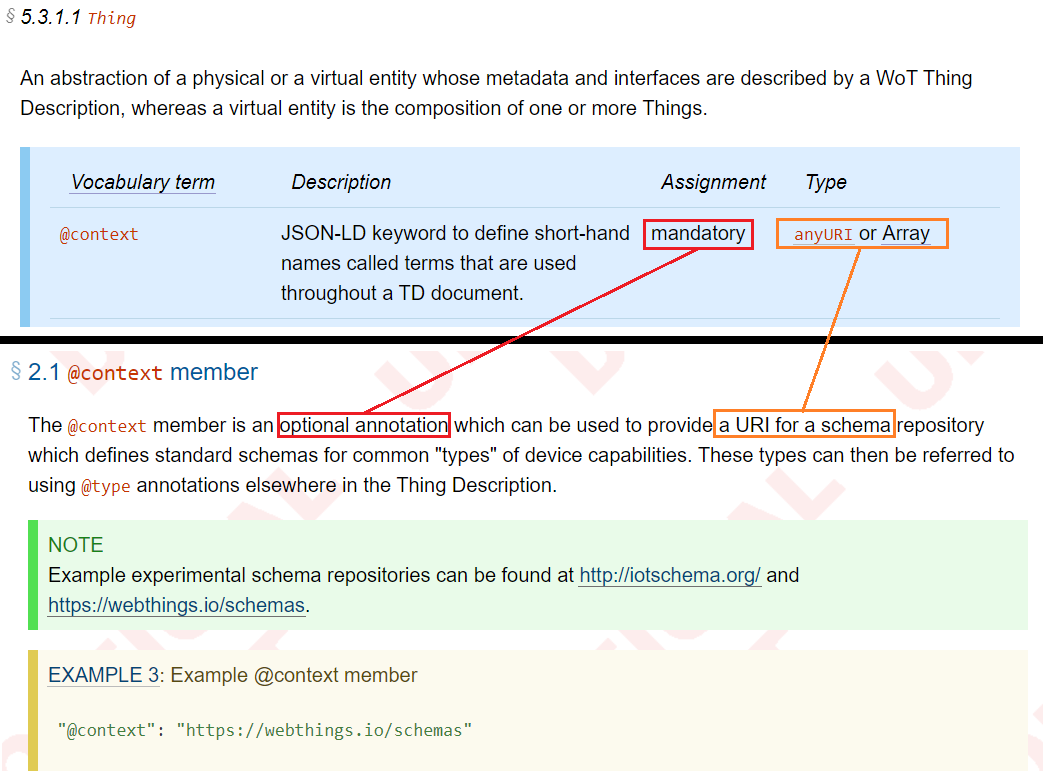
\includegraphics[scale=0.55]{eps/specification-conflict.png}
	\caption{Netto conflitto di specifiche tra \texttt{WebThings.io} e raccomandazioni del W3C.}
	\label{fig:specification-conflict}
\end{figure}

Come da figura \ref{fig:specification-conflict}, entrambe le definizioni collidono, e per puntualizzare il problema, si vuole sottolineare come \href{https://www.w3.org/TR/wot-thing-description/#example-28}{\ul{l'esempio 28}} del \href{https://www.w3.org/TR/wot-thing-description/#semantic-annotations}{\ul{capitolo 7.1}} della descrizione del W3C \textbf{\uline{NON}} sia compatibile con le specifiche di \texttt{WebThings.io}, e che quindi risulterebbe essere completamente illeggibile e inutilizzabile.\\

Rendere impossibile l'uso di ontologie, diverse da quella base, vanifica completamente l'obiettivo di questo progetto, per cui il framework di \texttt{WebThings.io} dev'essere necessariamente scartato. Si sottolinea però che direttamente sul suo repository ufficiale, è stato aperto un ticket di supporto\footnote{Issue 58 - \url{https://github.com/WebThingsIO/webthing-java/issues/58}} per richiedere questa funzionalità, che sarà probabilmente integrata in un prossimo futuro.

Come ultima nota, le differenze possono essere trovate sul seguente collegamento: \url{https://github.com/WebThingsIO/wiki/wiki/Mozilla-W3C-Differences}


\subsection{[TO DO] Yggdrasil}
Libreria creata pensando per un ambito più ampio, quello degli Agenti, ma che si adatta bene ad una classica programmazione grazie al fatto di essere una libreria Java per la creazione della Thing Description e, a differenza del framework di \texttt{WebThings.io}, risulta essere maggiormente compatibile con le indicazioni del W3C per quanto riguarda la definizione di quest'ultima.\\

La documentazione è reperibile soltanto dal repository stesso e risulta essere al livello nettamente inferiore rispetto a quella offerta da WebThings Framework. Il linguaggio utilizzato è soltanto Java, e quindi la scelta deve per forza ricadere su di esso (o eventualmente su linguaggi java-based, tipo Kotlin).\\

L'osservazione sulla compatibilità cade solo sulla versione di JSON-LD utilizzata, che nel caso di questo framework risulta essere la 1.0, mentre le specifiche del W3C indicano la 1.1 come riferimento ufficiale.


\subsection{Arena Web Hub}
Framework basato su Node.js contenente esempi di backend e frontend. È un tentativo di standardizzare protocolli differenti, in modo da creare interoperabilità tra essi: infatti, al suo interno, vengono implementati ben tre gateway (Web Hub, Mozilla Gateway e Eclipse Thing Web) che possono essere creati in modo da supportare differenti soluzioni. Le Things vengono create dopo che uno dei tre gateway è stato istanziato, chiamando il metodo \texttt{.produce()}, il quale come l'unico argomento prende in considerazione la Thing Description.\\

Il problema di questa implementazione è simile a quello descritto nella sezione \ref{sec:webthingsio}, trattante del framework di Web Things. Infatti, anche in questa implementazione non è chiaro il supporto per le annotazioni di ontologie diverse da quella standard. L'unica cosa citata nella documentazione è:

\begin{quote}
\textit{Note that the examples include a client-side Web of Things library (see "client/wot.js") with an adaptation layer for different Web of Things platforms. A further library is planned \ul{to make it easy to work with semantic annotations that describe the kinds of things (e.g. a light), their capabilities (e.g. dimmable), and the context in which they reside (e.g. my kitchen)}.}
\end{quote}

Analizzando il codice sorgente\footnote{\url{https://github.com/draggett/arena-webhub/blob/master/webhub.js}}, disponibile su GitHub e visibile in figura \ref{fig:context-overwritten}, è possibile comprendere che il supporto alle annotazioni è infatti \textbf{assente}, ma tecnicamente previsto. Il metodo \texttt{.produce()} sovrascrive tutti i parametri della Thing Description in modo da renderla conforme alle specifiche della libreria stessa, puntando il contesto a quello ufficiale specificato dall'ente W3C. In questo modo, ancora una volta, viene impedita la possibilità di collegarvi ulteriori ontologie e di definire una maggiore conoscenza sulla Thing descritta: infatti, non vi è alcun modo per aggiungerle successivamente e nell'oggetto che definisce la struttura delle Thing vi è una completa assenza del riferimento al contesto.\\

\begin{figure}[h]
	\centering
	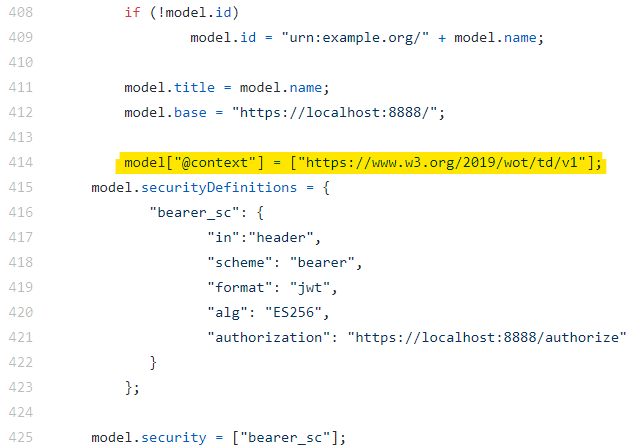
\includegraphics[scale=1]{eps/context_overwritten.png}
	\caption{La libreria implementata sovrascrive alcuni campi della Thing Description con i propri valori, rendendo inutilizzabili le ontologie eventualmente indicante nel contesto. Fonte: \url{https://github.com/draggett/arena-webhub/blob/master/webhub.js}, riga 414}
	\label{fig:context-overwritten}
\end{figure}

Similmente al framework di WebThings, nonostante un vasto supporto alle specifiche di W3C, non vi sono quelle richieste dai requisiti posti. Per questo motivo anche Arena Web Hub dev'essere scartato.


\clearpage
\subsection{ThingWeb.io}
Similmente ai framework trattati, come WebThings.io e Arena Web Hub, anche \textbf{ThingWeb.io} tenta di implementare gli standard raccomandati dal W3C. L'approccio in questo caso parte da un'implementazione Node.js: attraverso di quello si crea un endpoint, il quale poi potrà creare e o vedere Things create. Non vi sono particolari nozioni sul supporto alle ontologie aggiuntive (il problema maggiore delle precedenti soluzioni) e pare avere il supporto per la prototipazione e il lancio di Things virtuali. La documentazione esisten sia sul repository, sia nella pagina ufficiale del progetto.\\

Per controllare il supporto per i contesti, è necessario recarsi più a fondo nella documentazione: le specifiche riguardanti il primo lancio di una Thing all'interno di un Raspberry indicano come questa abbia al suo interno una Thing Description, che, come visibile dalla figura \ref{fig:context-ok-thingweb}, è completa di tutti i campi indicati nella raccomandazione del W3C, compresi alcuni aggiuntivi contesti rispetto a quello base.\\

\begin{figure}[h]
	\centering
	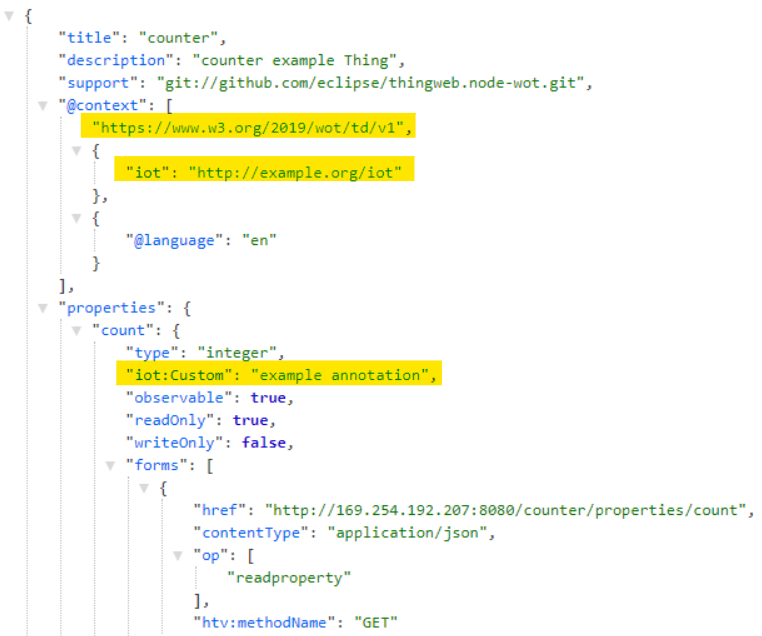
\includegraphics[scale=0.8]{eps/context_ok_thingweb.png}
	\caption{La Thing Description letta da ThingWeb risulta essere completa di tutti i campi. Sono evidenziati i contesti indicati e il loro utilizzo. Fonte: \url{http://www.thingweb.io/hands-on-intro-raspberry.html}}
	\label{fig:context-ok-thingweb}
\end{figure}

Per specificare meglio il supporto alla Thing Description, si può far riferimento al parser della TD, come nella figura \ref{fig:context-ok-thingweb_2}; in esso, quando viene incontrato il campo \texttt{@context} viene effettuato un controllo: in base alla tipologia del dato (stringa o array) vengono istanziate le rispettive risorse.\\

\begin{figure}[h]
	\centering
	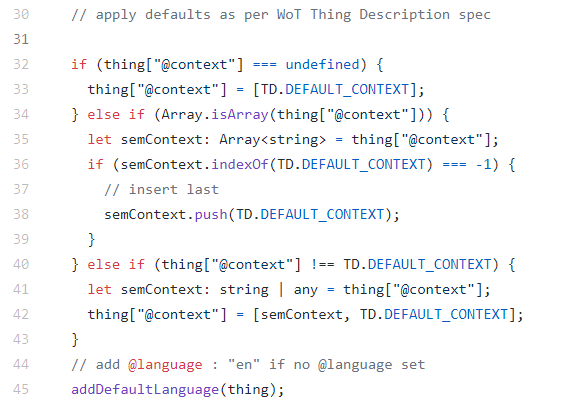
\includegraphics[scale=0.9]{eps/context_ok_thingweb_2.png}
	\caption{Nella riga 35 è chiaramente visibile il supporto a più definizioni di contesti. Fonte: \url{https://github.com/eclipse/thingweb.node-wot/blob/master/packages/td-tools/src/td-parser.ts}}
	\label{fig:context-ok-thingweb_2}
\end{figure}


Al momento, ThingWeb.io risulta essere l'unico framework capace di includere tutte le caratteristiche richieste dal progetto, per cui rimane il candidato principale.


\clearpage


\subsection{[TO DO] Analisi del framework scelto}

\begin{comment}
Mozilla WebThings offre due distinti moduli per la gestione e creazione delle Smart Things: il WebThings Gateway e WebThings Framework.\\

\textbf{WebThings Gateway} è un software che può essere lanciato all'interno di un Raspberry, sotto il sistema Linux oppure in ambiente Docker. Risulta essere il punto di controllo dell'intero sistema delle Things connesse, il quale si interfaccia con esse e permette il loro utilizzo. È utile sottolineare come questa soluzione sia adottata dalla maggior parte dei competitor sul mercato, con l'enorme differenza di avere, in questo caso, il pieno controllo su quello che è l'esecuzione e dati: il codice sorgente, infatti, risulta essere accessibile in tutte e tre le soluzioni. Inoltre, per puntualizzare alcuni aspetti tecnici, un \quotes{\textit{raccoglitore}} di questo tipo rappresenta, in un certo senso, un Single Point of Failure dell'intero sistema: dall'altra parte però risulta essere impensabile aggiungere della potenza computazionale ad oggetti come lampadine per permettere una strutturazione a rete completamente connessa tra oggetti, oppure, rendere il tutto perfettamente raggiungibile con collegamenti indiretti\footnote{anche se esistono protocolli di comunicazione che permettono un tale scambio di messaggi; questi necessitano però di un ulteriore hub per funzionare.}\\

Essendo il Gateway parte che permette la comunicazione tra gli oggetti, è essenziale poterlo tenere in esecuzione. Per fortuna, non vi è bisogno di una complessa configurazione per avviarlo e, come descritto prima, può essere lanciato su diverse piattaforme supportate.\\

\textbf{WebThings Framework} è una collezione di componenti riusabili che permettono la creazione delle Web Things: avendo definito nella sezione \ref{sec:webthing} che il sistema sviluppato si predilige meglio a supportare le \textbf{\ul{Web}} Things piuttosto che \textit{\ul{Smart}} Things, è un ottimo punto di partenza sapere che anche il nome stesso indica la correttezza della scelta effettuata. Una Web Thing può essere successivamente scoperta da un gateway o un client e può essere implementata in diversi modi e linguaggi:

\begin{itemize}
	\item \textbf{Mozilla Libraries}: librerie proposte direttamente da Mozilla, includenti NodeJs, Python, Java, Rust, Arduino.
	
	\item \textbf{Third Party Libraries}: librerie proposte direttamente dalla community, includenti Moddlable, Atmosphere, IoT.js, C\#, Go, ESP-IDF, PHP e Python.
\end{itemize}


Una volta definito precisamente il framework scelto, è opportuno delineare una strada da percorrere per il processo di sviluppo. La scelta è ampia e permette alla maggior parte dei programmatori a scegliere il modello che più si addice alle sue competenze e disponibilità di hardware: in questo caso le piattaforme prediligenti l'uso di device esterni, quali Raspberry o Arduino sono meno indicate, in quanto non attualmente in possesso.\\

Per poter comunque sperimentare la creazione di nuove Things, con l'annessa possibilità di prototipazione e test, è utile selezionare una delle modalità che permettono di ottenere il risultato richiesto anche nei requisiti definiti nel capitolo \ref{sec:iot_platform}. In base all'esperienza del programmatore, è più conveniente utilizzare la piattaforma \textbf{Java}, nella quale si hanno ormai consolidate conoscenze. Per non ricadere però in una classica implementazione, si preferisce adottare il linguaggio \textbf{Kotlin}, pienamente compatibile, per agevolare ulteriormente lo sviluppo.
\end{comment}


%%%%%%%%%%%%%%%%%%%%%%%%%%%%%%%%%%%%%%%%%non numera l'ultima pagina sinistra
\clearpage{\pagestyle{empty}\cleardoublepage}
\chapter{Implementazione delle Things}           %crea il capitolo
%%%%%%%%%%%%%%%%%%%%%%%%%%%%%%%%%%%%%%%%%imposta l'intestazione di pagina
\lhead[\fancyplain{}{\bfseries\thepage}]{\fancyplain{}{\bfseries\rightmark}}  

\section{Scelta dell'IDE}
Avendo scelto come linguaggio Kotlin, si procede alla configurazione dell'ambiente di sviluppo: in questo caso, vi è necessità di un IDE capace di facilitare lo sviluppo, considerando anche il linguaggio scelto. Esistono tre soluzioni più indicate in questo caso: Eclipse, IntelliJ e Visual Studio Code.\\

\textbf{Eclipse} è uno strumento gratis che permette un facile e agevole sviluppo in diversi linguaggi, tra cui il linguaggio Java. Anche se possiede il supporto a Koltin, esso non è nativo e a volte presenta dei problemi sia coi suggerimenti che con la compilazione.\\

\textbf{IntelliJ} è uno strumento versatile che permette uno sviluppo in diversi linguaggi, tra cui nativamente Java e Kotlin. Risulta essere la miglior scelta, anche se nella versione gratuita non offre tutte le funzionalità offerte nel pacchetto premium. La facilità con la quale però si integra con Kotlin, rende il suo utilizzo meno faticoso rispetto ad Eclipse.\\

\textbf{Visual Studio Code} è un editor di testo avanzato con diversi plugin per la maggior parte dei linguaggi conosciuti. È molto più povero delle due alternative proposte sopra: nonostante ciò è molto utile per il confronto dei file e per una veloce apertura dei file per l'esplorazione.\\

Mettendo in evidenza tutti i vantaggi e svantaggi, è chiaro che IntelliJ, se fosse nella versione premium, vincerebbe il primato della classifica. Essendoci però diversi problemi riguardanti il supporto di Kotlin su Eclipse è comunque preferibile utilizzare IntelliJ nella sua versione gratuita, per poter avere una rapida e indolore prototipazione di oggetti, senza perdere tempo sulla configurazione dell'ambiente di sviluppo. A parità di utilità, oltre a IntelliJ, si ritiene opportuno avere a disposizione Visual Studio Code per rapidi confronti e anteprime.\\





\begin{titlepage}
	\begin{center}
		\Large{DA QUESTO PUNTO IN POI LA RELAZIONE È IN BOZZA}
	\end{center}
\end{titlepage}









































\begin{comment}

%%%%%%%%%%%%%%%%%%%%%%%%%%%%%%%%%%%%%%%%%non numera l'ultima pagina sinistra
\clearpage{\pagestyle{empty}\cleardoublepage}
\chapter{Agenti e il mondo WoT}           %crea il capitolo
%%%%%%%%%%%%%%%%%%%%%%%%%%%%%%%%%%%%%%%%%imposta l'intestazione di pagina
\lhead[\fancyplain{}{\bfseries\thepage}]{\fancyplain{}{\bfseries\rightmark}}  

\section{Definizione di Agenti}
In letteratura, si possono trovare diversi esempi di definizioni di un Agente, due di esse citate di seguito:

\begin{quotation}
	\textit{
	An agent is a computer system that is situated in some
	environment and that is capable of autonomous action in
	this environment in order to meet its design
	objective” [Wooldridge \& Jennings, 1995]}
\end{quotation}

\begin{quotation}
	\textit{
	An agent is anything that can be viewed as perceiving its
	environment through sensors and acting upon the
	environment through effectors." [Russell \& Norvig, 1995]}
\end{quotation}

In poche parole, l'Agente risulta essere un'entità situata all'interno di un ambiente che riesce a percepirlo ed è capace di intraprendere azioni (anche autonome) per modificare il proprio stato (o quello dell'ambiente) attraverso l'uso delle sue capacità o degli oggetti che ha a disposizione, raggiungendo così i propri obiettivi.\\

Gli agenti possono essere classificati in diversi modi:
\begin{itemize}
	\item \textbf{accessible} (o inaccessible) - stabilisce se l'agente ha l'accesso allo stato completo dell'ambiente,
	
	\item \textbf{deterministico} (o non deterministico) - quando un cambio dello stato dell'ambiente è determinato univocamente dal suo stato attuale e le azioni eseguite dagli agenti,
	
	\item \textbf{statico} (o dinamico) - indica se lo stato dell'ambiente può cambiare a fronte di un azione dell'agente,
	
	\item \textbf{discreto} (o continuo) - specifica se il numero di percezioni e azioni sia limitato
	
	\item \textbf{centralizzato} (o distribuito) - stabilisce se il sistema degli agenti sè localizzato in una stessa struttura o meno,
	
	\item \textbf{generalizzato} (o specializzato) - indica se il sistema degli agenti  possiede delle azioni ben definite o indipendente dai tipi di azioni che possono essere svolte.
\end{itemize}


\subsection{Agenti BDI}
Calandosi nel contesto di studio, vengono definiti meglio quelli che sono Agenti BDI.\\

\textbf{BDI} è l'acronimo di \textit{\textbf{b}eliefs}, \textit{\textbf{d}esires}, \textit{\textbf{i}ntentions} (letteralmente "credenze, desideri, intenzioni") e definisce il modello secondo il quale vengono visti e definiti gli agenti. L'approccio seguito è basato su \textit{practical reasoning}, composto da due diverse fasi:

\begin{itemize}
	\setuldepth{come}
	\item \textbf{deliberation} - decidere \ul{quale} stato raggiungere o mantenere,
	\item \textbf{means-end reasoning} - decidere \ul{come} raggiungere o mantenere quello stato.
\end{itemize}

L'agente BDI è un'entità \textbf{proattiva}, persistendo nelle intenzioni che attualmente possiede e \textbf{reattiva}, nel caso in cui debba abbandonarle e/o cambiarle in seguito ad una modifica delle circostanze interne e/o esterne.\\

Per schematizzare il ciclo di esecuzione di un Agente BDI si può far riferimento alla seguente figura:

\begin{figure}[h]
	\centering
	\makebox[\textwidth][c]{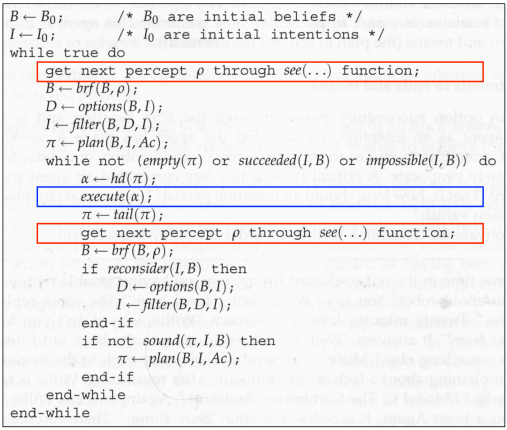
\includegraphics[width=1\textwidth]{eps/bdi-agent-cycle.png}}
	\caption{Ciclo di esecuzione di un Agente BDI.}
	\label{fig:jacamo}
\end{figure}

L'utilizzo di un Agente BDI ha bisogno di una sua codifica: per poter programmare gli agenti occorre utilizzare linguaggi come AgentSpeak, o meglio ancora Jason e vi è necessità di calarli all'interno di un ambiente definito, in quanto non è possibile utilizzarli esattamente come se fossero una \quotes{semplice} libreria: il modo in cui il programmatore deve interfacciarsi dunque sfrutta non più un classico paradigma, come quello ad oggetti, ma piuttosto reimmagina il sistema in una visione effettivamene ad Agenti.

\subsection{JaCaMo}
Come definito nella sezione precedente, gli Agenti hanno necessità di ritrovarsi all'interno di un ambiente per poter funzionare correttamente e poter parlare tra di loro. Esistono diverse librerie che permettono di istanziare environment pronti ad ospitarli, ma nel caso di studio si preferisce concentrare ad un particolare sistema basato sull'interazione Agenti-Artefatti-Ambiente chiamato JaCaMo.\\

\textbf{JaCaMo} \cite{jacamo} è un acronimo formato dall'incrocio di tre parole: Jason, CArtAgO \cite{cartago} e Moise \cite{moise}. Si tratta di tre componenti che interagiscono tra di loro per gestire al meglio un sistema ad Agenti. Ogni componente è responsabile di un compito:

\begin{itemize}
	\item \ul{Jason} si occupa della definizione di agenti,
	\item \ul{CArtAgO} gestisce la creazione degli Artefatti e la gestione della comunicazione Agente-Artefatto, il tutto grazie all'uso di Java
	\item \ul{Moise} definisce l'organizzazione degli agenti attraverso l'uso di file \textit{.xml}.
\end{itemize}

Tutto il pacchetto è strutturato in modo tale da far collaborare sempre un modulo con l'altro: si possono infatti mischiare i concetti ed estendere funzionalità degli agenti definendo alcune features a livello di Java e non solo tramite Jason. Bisogna però porre attenzione a non violare i principi di una buona programmazione ad agenti e trattare sempre le cose non-agent come delle blackbox da utilizzare soltanto in caso di estrema necessità, quando è impossibile scomporre ulteriormente il problema (ad esempio, una GUI non dovrebbe essere utilizzata direttamente all'interno di un Agente, ma necessita di essere un vero Agente/Artefatto con il quale gli altri agenti possono interfacciarsi).

\section{Agenti nel contesto IoT}

Il sistema ad Agenti nasce per diverse esigenze, che comprendono diversi ambiti. Il principale motivo per cui è più utile pensare ad un sistema eterogeneo organizzandolo più in modo Agent-Oriented è la completa indipendenza dell'esecuzione di ogni singolo componente (Agenti incapsulano anche il controllo, il ciclo di vita di uno è indipendente dagli altri) e la possibilità di astrarre a livello ancora più elevato rispetto alla OOP. Inoltre il modello ad Agenti offre la possibilità di rappresentare ancor da più vicino il mondo reale che ci circonda, in quanto questo è effettivamente formato da diverse entità (umani e/o macchine) che interagiscono continuamente tra di loro.\\

Parlando quindi soltanto in termini di praticità e progettazione, è già molto più facile per un programmatore immaginarsi le Smart Things come delle entità (Agenti/Artefatti) immersi dentro una stanza (Environment) che interagiscono tra di loro ed, eventualmente, hanno una gerarchia tale da permettere un pieno controllo delle azioni che vengono svolte all'interno dell'ambiente. Immaginando dunque di dover realizzare un sistema IoT, si pone davanti ad un problema di organizzazione delle Smart Things e della comunicazione tra di loro. Davanti ad uno studio di una Smart Room, si presuppone di avere alcuni oggetti Smart con le loro caratteristiche, con le quali l'utente può interagire. Dovendo pensare ad un modello ad alto livello, si può a produrre lo schema, visibile nella figura \ref{fig:use-case-diagram-high}, come illustrazione di ciò che potrebbe avvenire dentro questo ambiente.\\

\begin{figure}[h]
	\centering
	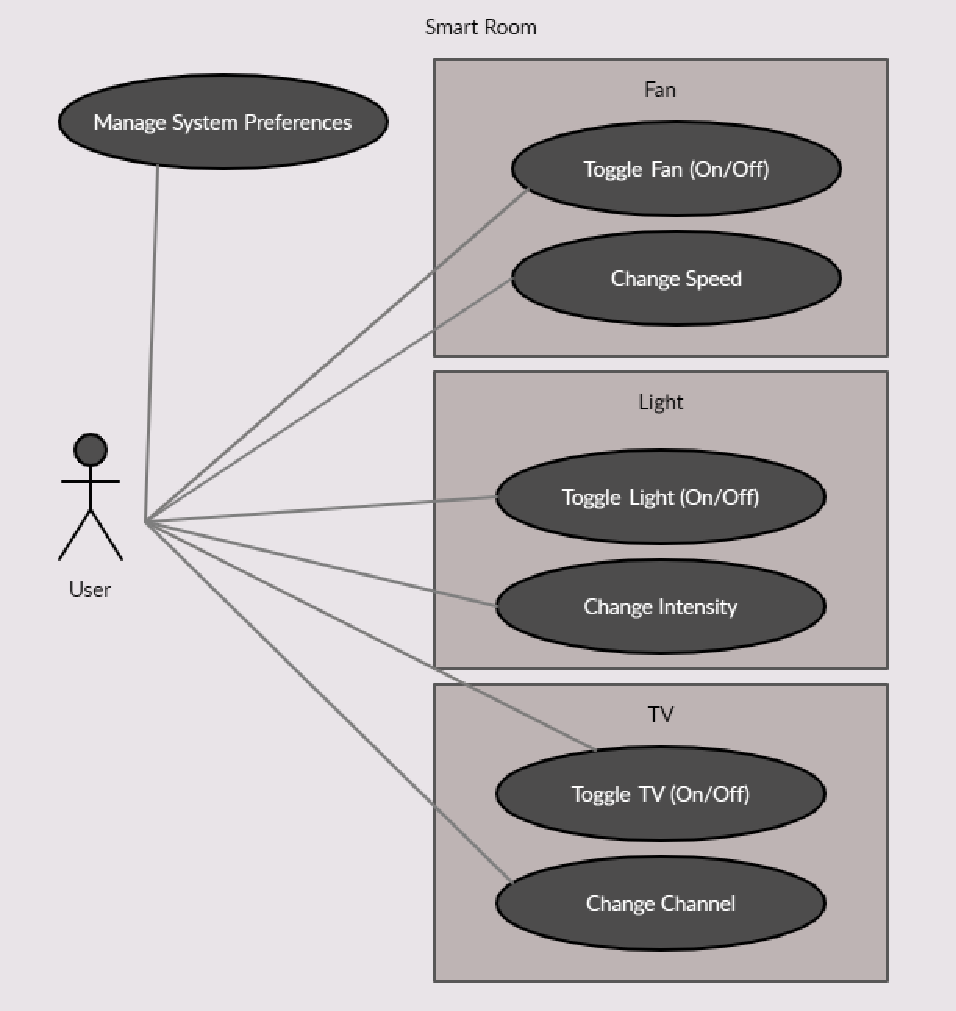
\includegraphics[scale=0.6]{eps/use-case-high.pdf}
	\caption{Rappresentazione ad alto livello di una Smart Room e suoi oggetti.}
	\label{fig:use-case-diagram-high}
\end{figure}

Pensandolo nel modo classico, ognuno dei sistemi rappresentati dovrebbe avere una classe che lo definisce, metodi con i quali posso interagire e caratteristiche specifiche per ogni singolo oggetto, eventualmente derivate. Una progettazione di classi rappresentative però non è l'unico step da eseguire, in quanto, successivamente, ognuna di esser dovrebbe esporre protocolli di comunicazione, dipendenti dall'oggetto in atto. Vi è poi necessità di un sistema che collezioni le istanze delle classi, e richiami opportunamente gli oggetti con il quale l'utente vuole interagire. Infine, è necessario poter vedere le preferenze dell'utente, in base alle quali gli oggetti immersi dentro il sistema dovrebbero poter (anche autonomamente) decidere come accontentare al meglio l'utente che le sta sfruttando. \\

Si può volgere di conseguenza lo sguardo alla descrizione presente sopra e calarla all'interno di un ambiente Agent-Oriented, dove i vari oggetti Smart sono Agenti/Artefatti. In questo modo si può astrarre ancor di più la progettazione, non calandosi direttamente alla rappresentazione tramite classi, ma proprio come entità del mondo vero calate quasi direttamente in quello ad Agenti. Come citato in \quotes{\textit{Agent-based modeling: Methods and techniques for simulating human systems}} \cite{abm}, la modellazione ad agenti possiede tre benefici:

\begin{itemize}
	\itemsep0em 
	\item cattura meglio i fenomeni che avvengono tra entità,
	\item fornisce una descrizione più naturale del sistema,
	\item risulta essere più flessibile.
\end{itemize}

È quindi di estrema semplicità immaginarsi un sistema Agent-Oriented ad alto livello, incentrato sulle interazioni Utene-Oggetti. Calandosi nel mondo JaCaMo, infatti, per ogni Smart Thing si può definire il suo Artefatto; successivamente, un agente addetto all'osservazione di questi potrà monitorare le preferenze dell'utente e interagire anche in modo autonomo con l'ambiente, per soddisfare eventuali esigenze. L'utente sarà facilitato nell'interazione con il sistema attraverso un'interfaccia grafica, potendo immettere comandi da eseguire.

\begin{figure}[h]
	\centering
	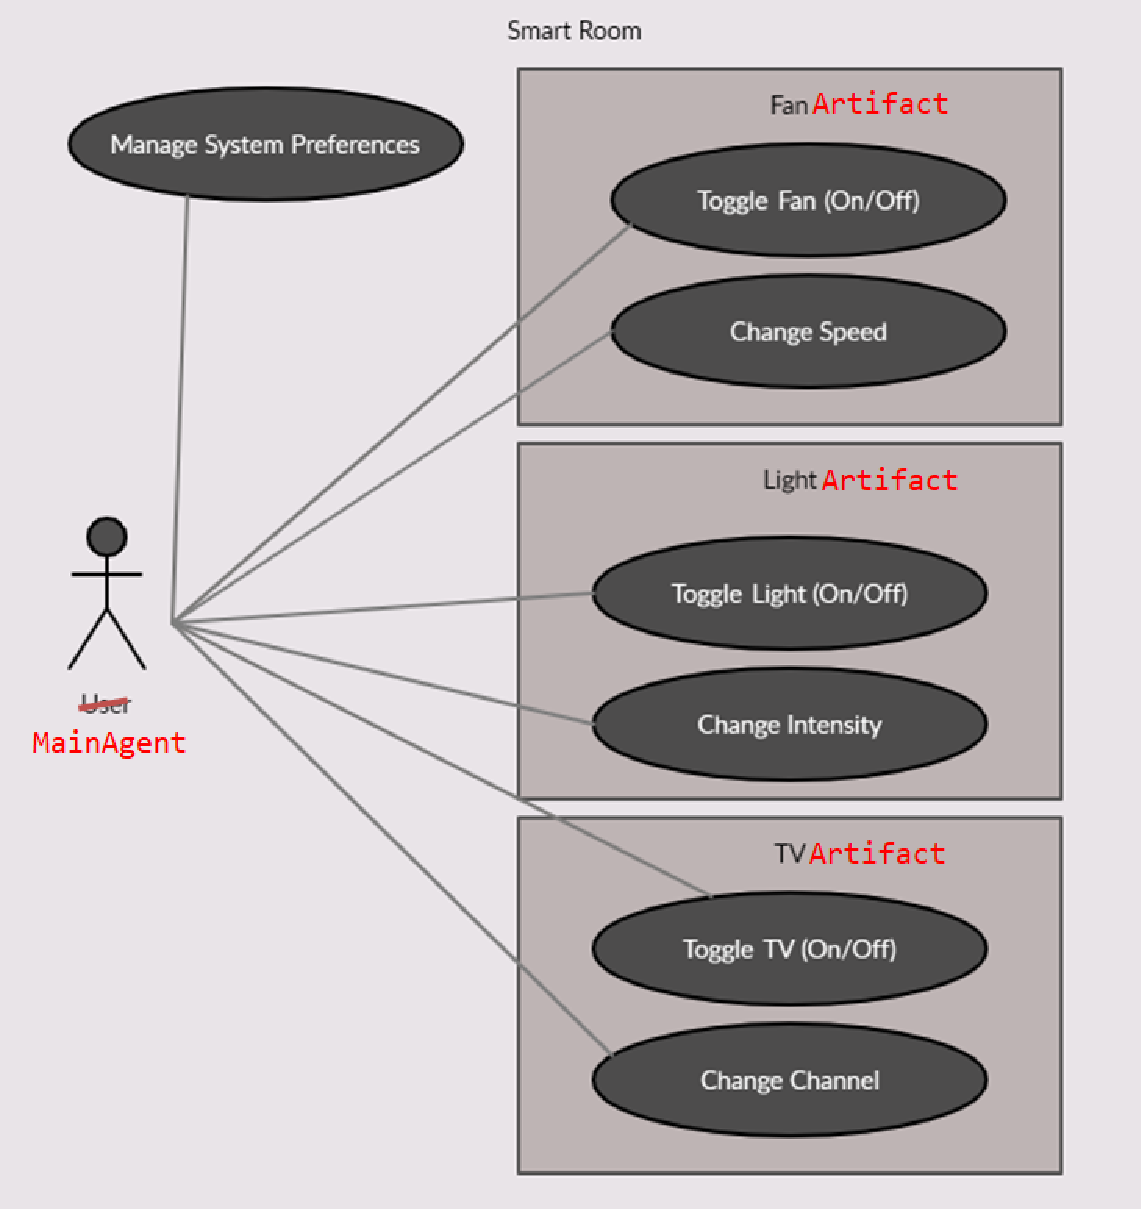
\includegraphics[scale=0.45]{eps/use-case-high-agent.pdf}
	\caption{Rappresentazione di una Smart Room e suoi oggetti rivisitata secondo il modello Agent-Based di JaCaMo.}
	\label{fig:use-case-diagram-high-agent}
\end{figure}

Come si può notare dalla figura \ref{fig:use-case-diagram-high-agent}, la progettazione di un sistema ad Agenti è direttamente mappata nel mondo reale. Ciò, come sottolineato in precedenza, porta ad un netto vantaggio sull'astrazione del sistema e sulla sua futura implementazione, in quanto nella visione Agent-Oriented tutto viene completamente incapsulato all'interno delle singole entità. Ovviamente, questa non risulta essere una completa progettazione: lo schema vuole dimostrare soltanto il diretto vantaggio che si ha sopra una progettazione classica ad Oggetti.\\

L'utilizzo del modello ad Agenti, inoltre, non riguarda soltanto semplici contesti come la Smart Room: vi sono infatti presenti studi che spaziano argomenti riguardanti sistemi di evacuazione \cite{evacuation} o addirittura l'osservazione delle api \cite{bee}.

\section{BDI e Smart Things}
Come da definizione, il modello BDI si basa sui concetti di \textit{\textbf{b}eliefs}, \textit{\textbf{d}esires} e \textit{\textbf{i}ntentions}. Vi è necessità di analisi per quanto riguarda le seguenti affermazioni e quali sono i vantaggi (e/o svantaggi) di utilizzare questa metodologia per lo sviluppo di un sistema IoT.\\

Come citato da \textit{\quotes{MATCH: MultiAgent-based Tactful CooperationScheme for Heterogeneous IoT Devices}} \cite{masiot}, utilizzare agenti può determinare una semplificazione della gestione per quanto riguarda l'eterogeneità delle cose naturalmente presenti in un ambiente, dati diversi contesti nei quali un sistema ad Agenti può essere applicato. Bisogna però saper specificare con criteri rigorosi i comportamenti che le cose debbano avere, in modo da garantire sia la sicurezza delle persone che il risultato atteso, portando ad una collaborazione (e non competizione) tra le cose che si hanno a disposizione.

\subsection{Ordine ed esecuzione delle azioni}
In primo luogo, la capacità degli Agenti ad essere predisposti a interagire tra di loro, anche autonomamente, risulta essere un netto (teorico) vantaggio per quanto riguarda l'implementazione di un sistema Smart: il modello a scambio di messaggi abbraccia completamente la natura asincrona negli eventi che possono capitare all'interno di un ambiente, ma bisogna essere precisi nello specifico sulle priorità dei messaggi in arrivo. Di default, infatti, non vi è implementato un modo per ordinare i messaggi che un Agente si vede arrivare.\\

Per questo motivo vi sono presenti strumenti per gestire la priorità delle azioni: è necessario però porre attenzione a non disporre i controlli all'interno dell'Agente stesso, ma nella parte relativa alla ricezione e gestione messaggi. L'agente, infatti, deve poter eseguire le proprie intenzioni anche in assenza di alcune conoscenze, se questo vi è permesso: la belief (iniziale e imparata) è esattamente il motivo per il quale ciò è possibile, se ovviamente l'entità è capace di valutare con accuratezza la situazione dell'ambiente in cui si trova.\\

Non bisogna però intendere questo come una carta bianca per gli Agenti ad eseguire azioni che ritengono giuste: è compito del programmatore a rendere le singole entità sicure, in modo da poter interrompere operazioni, anche critiche, nel caso di uno o più fallimenti. Gli Agenti sono infatti liberi di crearne delle nuovi (o nel caso di JaCaMo, di creare nuovi Artefatti) e di eliminarli a dovere: quest'ultima viene vista come un'operazione importante, in quanto l'eliminazione di una entità provoca automaticamente la distruzione di tutte quelle sottostanti nella sua gerarchia.\\

L'autoregolazione del sistema, quindi, è frutto di conoscenza degli Agenti ed esperienza del programmatore a renderli autonomi e capaci di imparare. Grazie all'utilizzo di tutti gli strumenti dati a disposizione, gli ambienti possono così diventare più propensi ad essere effettivamente \quotes{Smart}, non perchè un'azienda ha deciso di etichettarlo così, ma per definizione di quello che quel determinato sistema può fare e offrire nel suo insieme. Dall'altra parte, è da considerare una visione distopica, dove troppe cose eseguite da macchine rendono uomini meno capaci a svolgere anche banali compiti, diventando quindi completamente dipendenti dalla tecnologia.

\subsection{Agente come entità centrale}
La \textit{belief} di un Agente è quello che egli sa sull'ambiente in cui si trova, sia che si tratti di ulteriori entità, sia che dell'ambiente stesso. Nel caso di una Stanza Smart, questo può essere visto come un vantaggio in termini di completo monitoraggio del sistema implementato; dall'altra parte però utilizzando un'unica figura centrale come Agente, che si interfaccia poi con tutte le Things implementate come Artefatti, potrebbe portare ad un Single Point of Failure, dove se l'entità centrale smette di funzionare, anche tutte quelle ad essa sottostanti non rispondono più ai comandi.\\

Si potrebbe quindi ragionare piuttosto ad un sistema che, dati gli oggetti Smart, conferisca all'utente un'unica interfaccia nella quale sono disponibili tutti gli oggetti, ma anche una possibilità di controllare direttamente le Smart Thigs, senza l'ausilio di un ente centrale per il quale si debba per forza passare. Il problema di questa soluzione è la difficoltà nell'implementazione: infatti, ogni singolo oggetto non è più solo un Artefatto osservabile, ma di fatto un Agente Intelligente. Un ulteriore problema di questa soluzione risulta essere proprio il trattamento delle Smart Things come entità autonome: non è detto che sia necessario avere una lampadina vista come un'entità così Smart da decidere in autonomia che piano intraprendere in base allo stato dell'environment in cui si trova, anche perchè questo vorrebbe dire che ogni Thing debba essere connessa all'altra, per scoprire perfettamente lo stato del sistema. Tenere un'unità centrale vanificherebbe il tentativo di decentralizzazione, anche perchè si ritornerebbe nel precedente caso nel quale tutte le informazioni debbano passare da una singola struttura centrale.\\

\begin{figure}[h]
	\centering
	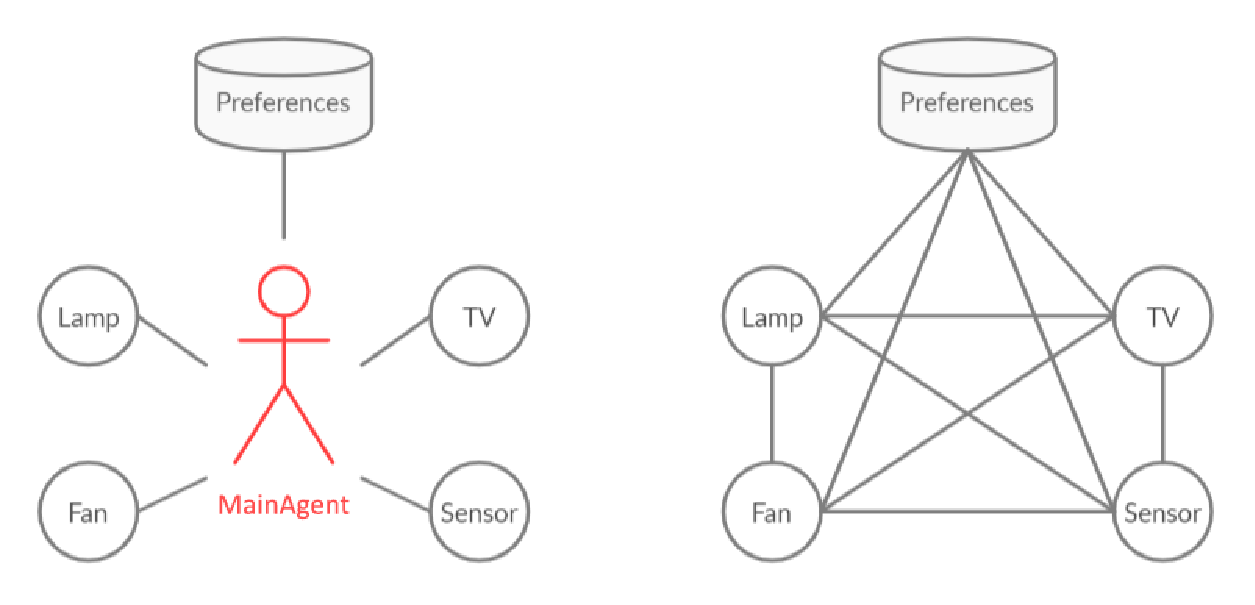
\includegraphics[scale=0.6]{eps/spof.pdf}
	\caption{Differenza tra un sistema centralizzato e decentralizzato. Si può vedere al colpo d'occhio la semplicità e la criticità del primo, e la complessità del secondo, oltretutto, al crescere dei dispositivi connessi.}
	\label{fig:spof}
\end{figure}

Da una parte quindi si ha il problema della molteplicità di comunicazione, che cresce esponenzialmente con l'aggiunta di nuovi dispositivi, che però rispecchia pienamente la decentralizzazione di un sistema ad Agenti; dall'altra un \textit{SPOF} che semplifica nettamente la gestione dell'intero ambiente e permette di concentrare le operazioni importanti all'interno di una singola entità, favorendo l'eventuale collaborazione e il discovery delle nuove funzionalità, non incrementando nello stesso momento le capacità di azione individuale delle Smart Things.
Dipendentemente quindi da cosa si vuole ottenere dal sistema, è opportuno scegliere una delle due strade. Essendo però la seconda, quella centralizzata, più facile da implementare e scalabile (in un sistema da 10.000 oggetti è impensabile infatti rendere ogni oggetto responsabile di osservare l'interno ambiente e capire l'azione da intraprendere, mentre con l'entità centrale è lei a doversi preoccupare di tutto), per quanto riguarda la scelta per le successive fasi di analisi, si preferisce pensare al sistema Agent-Based con un Agente centrale che \quotes{comanda} gli Artefatti.

\subsection{Things e Agenti}
Non solo la \textit{belief}, ma anche \textit{desires} e \textit{intentions} riguardano da vicino l'analisi che dev'essere affrontata. Mentre è logico infatti pensare all'agente centrale che si pone come desiderio e/o intenzione quella di voler illuminare la stanza, è più difficile calarsi a più basso livello supponendo che una lampadina abbia il desiderio e/o intenzione di accendersi o cambiare la sua intensità.\\

Vi è però necessità di differenziare quello che idealmente un sistema ad Agenti potrebbe essere e quello che si sta cercando di realizzare. Nel contesto attuale si sta pensando ad un modo per interfacciare le Smart Things esistenti sul mercato in modo da poterle inserire dentro una stanza e utilizzare per questo scopo Agenti BDI. La Thing, di per sè, è stata già progettata, realizzata; ha già feature interne che le permettono di cambiare il loro stato interno: queste però \textbf{non} sono state progettate in vista di un'applicazione in un sistema Agent-Based, ma piuttosto in un ambiente Smart classico tramite connessione ad un Hub WiFi (o altri, ad esempio ZigBee).
Ponendo caso che si voglia realizzare una Smart Thing da 0, utilizzando sin da subito il paradigma Agent-Based, viene automatico pensare alla lampadina come se fosse effettivamente un agente: ha delle intenzioni, dei desideri e delle credenze su quello che è il sistema \quotes{Lampadina}. Per essere Smart ha sicuramente bisogno non solo delle parti elettriche che permettono di emanare luce, ma anche quelle di ricevere comunicazioni dall'esterno, di managing energetico interno e simili. Dunque, è logico in questo caso contraddire l'introduzione di questa sezione: infatti, se guardata internamente e realizzata dall'inizio con questa ideologia, la lampadina \textbf{può} essere sviluppata seguendo questo paradigma, avendo quindi tutte le cose che caratterizzano un Agente. Di conseguenza, anche l'intero sistema dovrebbe essere rivalutato in modo da inglobare non solo Artefatti che si interfacciano con le Things già esistenti, ma anche l'unità centrale che deve riconoscere ulteriori Agenti come Smart Things.\\

Come però sottolineato, questo è solo un caso ipotetico. Attualmente non vi sono particolari sviluppi nell'ambito Smart Things che prevedono l'utilizzo della Programmazione ad Agenti intensiva, e la maggior parte delle Things esistenti non è stata pensata per farne uso. Per questo motivo se si volesse realizzare un sistema completamente ad Agenti, vi è necessità di progettare e realizzare anche Smart Things seguendo lo stesso modello; nel caso di studio, invece, si tratterà di un approccio più limitato, che si baserà sull'adozione di Smart Things correntemente esistenti e funzionanti, senza dover inventare nuovi metodo per la creazione delle entità Smart.\\

Inoltre, come descritto in \textit{\quotes{Building Cyber-Physical Systems - A Smart Building Use Case}} \cite{smartbuilding}, anche una semplice casa possiede diverse sfide, sia per quanto riguardo l'eterogeneità delle cose che la complessità delle azioni da compiere. Vi sono infatti diversi strati di interoperabilità che possono esistere. Dall'altra parte, seppur non citando direttamente, l'articolo fa anche riferimento all'uso di ontologie (o comunque tecnologie standard) per quando riguarda il layer della descrizione degli oggetti e del loro stato, ricadendo perfettamente nell'ambito di studio qui presentato, trattato poi successivamente nel capitolo \ref{sec:td}.

\subsection{Blackboxes}
Nella precedente sezione è emerso un dettaglio molto importante riguardante la natura non-Agent-friendly delle entità che si vorrebbe in qualche modo sfruttare all'interno del sistema. Un Agente, infatti, è autorizzato a comunicare soltanto grazie allo scambio di messaggi, non tramite il richiamo di alcuni metodi, ne tramite l'uso di tecnologie com RPC o altre, come WebSocket.\\

In JaCaMo questo problema è stato superato grazie all'adozione degli Artefatti: attraverso di essi, infatti, è possibile interagire con del codice legacy (o delle classi/librerie o addirittura programmi interi), rendendo le cose completamente trasparenti dal lato dell'Agente che osserva quell'Artefatto. Ovviamente, si tratta di un processo di "blackboxing" di quella che è la vera natura dell'oggetto interessato, ma senza di esso la Agent Oriented Programming non potrebbe dichiararsi priva di codice \quotes{sporco} di qualche richiamo della classica OOP.\\

L'artefatto dunque può nascondere l'entità di una qualsiasi parte già implementata: una GUI in JavaFX, una Smart Things con un display e una stampante appaiano tutte come un Artefatto, il quale con le sue azioni interne permette all'Agente di mandargli i messaggi. L'agente risulta essere quindi compliant allo standard di programmazione, e l'artefatto gestisce la richiesta interamente per essere compliant con la tecnologia che viene sfruttata sotto.\\

Questo problema può essere visto in duplice modo: da una parte vi è una complicazione per i programmatori per rendere le cose più separate e non immediatamente disponibili, dall'altra, come nella programmazione ad Oggetti, è una buona pratica non far fare troppo ad una sola entità; infatti, al crescere di eventuali features è probabile che si assista più ad un caos che ad una semplificazione dei problemi, per cui lo svantaggio descritto risulta essere in realtà più un vantaggio, che permette di mantenere il principio di separazione degli obiettivi, rispettando inoltre gli standard della programmazione ad Agenti.

\subsection{Sicurezza}
Come citato in \quotes{\textit{Intelligent Multi-Agent Collaboration Model for Smart Home IoT Security} \cite{security}}, gli agenti possono essere utilizzati anche per incrementare la sicurezza dei sistemi IoT. Utilizzando infatti una strutturazione a base di molteplici agenti che creano un layer di trust in base al database sottostante, si può ottenere una organizzazione interna tale da permettere un maggiore controllo su chi esegue i comandi (soprattutto da remoto).\\

Per motivi di semplicità la soluzione proposta non verrà adottata nel risultato finale, tuttavia si sottolinea l'importanza e l'esistenza di tale studio.


\section{Disponibilità della conoscenza}
In una visione completa di un sistema, nel quale si può immaginare un numero potenzialmente infinito di oggetti Smart, è naturale aver a che fare con una molteplicità di informazioni e operazioni da fare che necessariamente ha bisogno di essere in qualche modo regolamentata e strutturata, in modo da evitare il caos che ne deriverebbe. Le problematiche, infatti, non riguardano soltanto la quasi impossibilità di manutenzione del sistema, dovuta alla scarsa interoperabilità dei sistemi, ma anche la semplice osservazione e raccolta dati dell'ambiente in cui questo fantomatico sistema potrebbe funzionare. In poche parole, l'applicazione caotica e senza regole di un sistema eterogeneo porta inevitabilmente alla lenta distruzione dello stesso, vanificando completamente le soluzioni ai problemi che si erano posti di risolvere.


\subsection{Thing Description}
\label{sec:td}
Da diverso tempo si sta discutendo su come rendere il mondo IoT più versatile, compatibile, universale e aperto. Le attuali tecnologia risultano essere perlopiù proprietarie e non standardizzate, per cui si è spesso costretti a rimanere legati con uno (o pochi) competitor presenti sul mercato per problemi di compatibilità dei sistemi. Infatti, ogni oggetto Smart attualmente presente sul mercato, ha bisogno di un suo centro di comando, che differisce da produttore a produttore: nel caso di oggeti Smart dotati di protocolli WiFi generalmente basta un'applicazione che riesca a sfruttare il protocollo REST; ma utilizzato protocolli come Bluetooth e/o ZigBee ogni manufacturer implementa un suo protocollo di comunicazione che non è noto a priori.\\

Per far fronte alle diversità e per regolare il caos che si sta cominciando a creare, anche in vista dell'imminente espansione di oggetti Smart, grazie anche all'introduzione delle nuove infrastrutture, soprattutto quelle di comunicazione, l'ente W3C \cite{w3c} ha instaurato il Web Of Things \cite{wot} e la Thing Description \cite{td}, argomenti già trattati nel capitolo \ref{sec:w3c}.\\

L'uso della Thing Description facilita la discovery e l'interoperabilità tra gli oggetti presenti nell'ambiente. Avendo al suo interno attributi, azioni, proprietà osservabili dell'oggetto e l'insieme delle cose human e non-human readable, permette di avere un quadro completo di quello che l'oggetto può essere e di quello che può svolgere.\\

Calandosi nel mondo degli Agenti, è facile pensare ad una creazione dinamica delle Things per inserirle all'interno del sistema. È necessario quindi definire alcuni passi fondamentali per eseguire completamente il processo di creazione e inserimento di una nuova Thing all'interno di un ambiente:

\begin{enumerate}
	\item \textbf{Utente aziona il comando \textit{Add New Thing}}: tramite un'interfaccia grafica presente in un'App o in una Smart Thing l'utente dichiara la volontà al sistema di voler aggiungere una nuova Smart Thing.
	
	\item \textbf{Agente cattura il comando}: l'entità centrale che si occupa della gestione capisce che un nuovo oggetto sta per essere inserito. Chiede all'utente gli unici due dettagli che vuole sapere: il nome della cosa e la sua Thing Description.
	
	\item \textbf{Agente crea l'artefatto con la TD}: una volta ottenuto i dati, l'agente chiede la creazione di un nuovo artefatto con il nome indicato dall'utente, che rispecchia l'oggetto reale grazie alla Thing Description.
	
	\item \textbf{L'Artefatto si dichiara pronto}: esso comunica all'Agente di poter essere testato da parte dell'utente prima di dichiararsi completamente funzionante.
	
	\item \textbf{L'Agente vede l'artefatto}: dopo aver ricevuto la sua richiesta, l'agente comunica all'utente che sarebbe meglio se guardasse la Smart Thing appena aggiunta e che ne verificasse le funzionalità.
	
	\item \textbf{Verifica delle funzionalità}: l'utente è libero di testare, approvare e/o modificare il comportamento della Thing appena creata.
\end{enumerate}

Questi passaggi risultano essere una proposta di algoritmo che potrebbe servire all'istanziamento di una nuova Thing nell'ambito di una Smart Room Agent-Based, supponendo di voler realizzare il sistema con l'Agente centrale che comanda la Smart Room. Mentre quasi tutti i punti sono realizzabili utilizzando metodologie date allo sviluppatore, sia attraverso le API di JaCaMo, sia attraverso l'uso di librerie Java, vi si possono trovare alcuni punti critici di questo procedimento:

\begin{itemize}
	\item \textbf{Limiti di JaCaMo a Runtime}: anche se esistono (o comunque possono essere implementati) metodi per il parsing della Thing Description, attualmente l'ambiente di JaCaMo non offre nessuna possibilità di aggiungere proprietà e azioni eseguibili a runtime, vanificando completamente l'obiettivo di creare dinamicamente delle Things. 
	
	\item \textbf{Conoscenza delle funzionalità}: non solo l'Artefatto, ma anche l'Agente che lo osserva ha bisogno di sapere quali sono le funzionalità derivate dalla Thing Description letta. Il problema si può risolvere in due modi:
	
	\begin{itemize}
		\item L'Agente si occupa di leggere la TD, in modo da capirne le funzionalità. L'Artefatto quindi viene creato dopo che la descrizione dell'oggetto venga letta. In questo modo si fa svolgere tutto il lavoro all'Agente, rompendo il principio della Single Responsibility.
		
		\item L'Artefatto, una volta pronto dopo aver letto la TD, dichiara all'Agente quali sono i metodi che l'Agente può chiamare su di lui. Questo punto però interferisce con i limiti che esistono al momento con JaCaMo sull'esecuzione a Runtime.
	\end{itemize}
	
	\item \textbf{Necessità dell'intervento umano}: l'approvazione da parte dell'utente potrebbe essere macchinosa, soprattutto se si dovessero aggiungere centinaia di Things. Si potrebbe pensare ad un meccanismo di automazione del test della Thing, che capisce in qualche modo di essere configurata bene (ad esempio, configurando una lampadina si potrebbe pensare di creare, a partire dalle proprietà e azioni comprese, un test automatico che verifica tutte le funzionalità apprese, come accendi/spegni/regola intensità e simili). Questo processo può essere ritenuto non critico in un ambiente casalingo, mentre nell'ambito industriale è di estrema importanza garantire la sicurezza dei dipendenti e delle macchine.
	
	\item \textbf{Necessità della configurazione manuale}: l'intero processo potrebbe essere semplificato, se le Smart Things avessero modo di comunicare automaticamente i loro nomi e il percorso per la Thing Description. In alternativa, ogni Smart Thing dovrebbe avere un percorso standard dove trovare il proprio nome e la TD, in modo che, una volta accese, possano essere automaticamente rilevate dall'Agente centrale e configurate senza che l'utente debba per forza dichiarare di voler aggiungere una nuova Thing.
	
	\item \textbf{Mancanza di standard evoluti/in uso/noti}: anche se si disponesse di tutte le tecnologie che permettono la realizzazione di tutti i punti precedenti, un'ultima nota dolente, per quanto riguarda la situazione attuale, è la completa mancanza delle Thing Description per le Smart Things correntemente esistenti. Essendo uno standard nuovo e non particolarmente usato (anche perchè ogni brand vuole tenersi l'utente stretto alle proprie soluzioni), vi è necessità di creazione manuale delle TD per gli oggetti che si vogliono creare. Il vantaggi ottenuti sono principalmente due: non solo si comincia ad utilizzare uno standard approvato, ma ulteriormente, si può pensare alla realizzazione di un database accessibile a tutti, nel quale vengono raccolte e pubblicate le TD realizzate da parte di tutti gli utenti da tutto il mondo, facilitando, con il passare del tempo, la configurazione all'interno dei sistemi che sfruttano la Thing Description (non per forza soltanto quelli ad Agenti).
\end{itemize}


Nel frattempo, JaCaMo si sta evolvendo e metodologie che permettono tali operazioni sono in via di arrivo. Per motivi didattici e di tempo, nell'eventualità di realizzazione un proof of concept, si preferirà predisporre di tutte le cose attualmente implementabili, lasciando spazio alle successive aggiunte e/o modifiche post-aggiornamento, simulando, per il momento, alcuni dei comportamenti non ancora implementati e/o che richiederebbero la realizzazione di un progetto complesso a parte, non rientrante nei temi che si vorrebbero affrontare con questo studio.

\subsection{Thing Status}
Mentre è possibile definire interamente le proprietà e azioni di una Thing attraverso la TD, sarebbe utile se si potesse, allo stesso modo, descriverne lo stato attuale. La Thing Description, infatti, copre soltanto il lato \quotes{statico} della Thing, specificando unicamente quelli che possono essere aspetti osservabili ed eseguibili, ma non quelli attualmente attivi.\\

Non esistono attualmente standard che permettono di definire lo stato attuale di una Thing. Si può immaginare però, ad esempio, che tutte le proprietà osservabili di un Artefatto, che una Thing di conseguenza possiede, possano essere in qualche modo tradotte in un formato standard, ad esempio in RDF. Utilizzando il modello così definito, ogni entità presente all'interno di un ambiente potrebbe fornire non solo la sua descrizione, intesa come il \quotes{\textit{cosa so fare}} ma anche il \quotes{\textit{come sto ora}}.\\

La questione, inizialmente, risulta essere banale se osservata da solo un punto di vista: le Things hanno già modo di dire al sistema in che situazione attualmente si trovano e di comunicare i cambiamenti in Real Time grazie ad uno scambio di messaggi. Servire un ulteriore modo per descrivere ciò di cui si ha già disposizione sembra un controsenso, eppure vista dall'alto può essere uno strumento utile per diversi motivi:

\begin{itemize}
	\item \textbf{Utilizzo standard di dati}: avendo a disposizione l'informazione su tutto il sistema in un formato unico e standard, è possibile sfruttare la conoscenza in possesso per eseguire ulteriori analisi, ottimizzazioni, statistiche e quant'altro. In poche parole, l'utilizzo di una rappresentazione comune a tutti facilita quello che è l'osservazione continua del sistema, dal puro punto di vista dei dati e risultati ottenuti.
	
	\item \textbf{Snapshot}: un fantomatico sistema in funzione potrebbe decidere di eseguire il monitoraggio completo delle risorse che ha a disposizione, salvando man mano lo storico di quello che era lo stato delle varie entità nel tempo. Questo può essere utile per la fase di debug o quando si verificano i guasti: un operatore può andare indietro nello storico e guardare tutti i parametri di tutte le entità connesse tra di loro e individuare eventuali criticità. Nel sistema ad Agenti, questa operazione può essere ulteriormente semplificata, prendendo automaticamente decisioni in base alle circostanze globali dell'ambiente, avvertendo eventualmente gli operatori delle azioni critiche intraprese.
	
	\item \textbf{Scoperta nuove funzionalità}: un sistema descritto in modo tale da permettere ad una macchina di fare del reasoning sopra, rende possibile la scoperta di ulteriori funzionalità (o proprietà) del sistema, non inizialmente previste. Sapendo, ad esempio, di avere 4 lampadine connesse in fila, si può dedurre che accendendo e spegnendole in un certo ordine si possono creare sequenze di luci. Nel caso di un entità centrale, ad esempio, il reasoning potrebbe essere fatto ogni tal volta che un nuovo oggetto viene aggiunto al sistema, ragionando su quelle che sono le azioni e proprietà di quell'oggetto.
	
	\item \textbf{Sicurezza}: analizzando i dati a disposizione, eventualmente derivandone nuovi, si possono individuare pattern comportamentali di individui che utilizzano quotidianamente oggetti Smart. Grazie alla descrizione dello stato, essa è univoca e osservabile sempre: se un malintenzionato volesse procedere in modo molto contrastante con quelle che sono le solite abitudini degli utilizzatori, il sistema potrebbe provvedere all'avviso o addirittura blocco delle azioni malevole. Inoltre, la verifica sui comportamenti dei singoli oggetti, analizzando il loro stato, porta ad un'incremento dell'affidabilità degli stessi, nonché aggiunge uno strato di protezione contro Things malevole, che senza un monitoraggio attivo del loro stato attuale, potrebbero essere immerse nel sistema e risultare invisibili e/o camuffate; ad esempio, conoscendo un classico comportamento di una lampadina, se essa cominciasse ad eseguire azioni non comuni a questa tipologia di oggetto, il sistema potrebbe avvisare l'utente e/o bloccare un tale azione.
	
	\item \textbf{Individuazione oggetti}: nel caso in cui la Thing Description non fosse disponibile, oppure nel caso in cui non sia completa, avendo a disposizione una quantità di dati sufficiente, è possibile non solo individuare pattern comportamentali di oggetti, ma anche oggetti stessi, permettendo la loro corretta classificazione. Questo aspetto può portare ad una semplificazione di interrogazioni che potrebbero essere fatte all'interno dell'ambiente, chiedendo, ad esempio, di elencare tutti i dispositivi le cui funzionalità corrispondono ad una determinata interessata caratteristica. Questo aspetto è comunque strettamente legato a tutto quello che è descritto già nel punto soprastante, riguardante la sicurezza.
	
\end{itemize}

Dare semantica agli oggetti quindi, non solo nel modello degli Agenti BDI, vuol dire aggiungere potenzialità e nuove possibilità all'environment analizzato: rendere le cose ancora più connesse e parlanti, garantendo, oltretutto, un maggior controllo su quello che succede all'interno del sistema incrementandone la sicurezza; il tutto porterebbe ad una riduzione dei costi di manutenzione, prevenzione dei guasti e/o la limitazione dei danni dovuti ad essi, nonché garantirebbe una vasta disponibilità di dati che possono essere marcati come \quotes{\textit{smart}}, in quanto ben definibili, collegabili e capibili da una macchina.\\


Purtroppo attualmente in campo non esistono standard che definiscono questo tipo di soluzioni, anche se come descritto in \textit{\quotes{Building Cyber-Physical Systems - A Smart BuildingUse Case}} \cite{smartbuilding}, si può però pensare di poter usufruire delle ontologie definite, ad esempio, tramite RDF \cite{rdf}. Per realizzare un test di quello che viene poi definito, si può pensare a SPARQL \cite{sparql} per quanto riguarda l'interrogazione della conoscenza creata.



%%%%%%%%%%%%%%%%%%%%%%%%%%%%%%%%%%%%%%%%%non numera l'ultima pagina sinistra
\clearpage{\pagestyle{empty}\cleardoublepage}
\chapter{Proof of Concept - Design}           %crea il capitolo
%%%%%%%%%%%%%%%%%%%%%%%%%%%%%%%%%%%%%%%%%imposta l'intestazione di pagina
\lhead[\fancyplain{}{\bfseries\thepage}]{\fancyplain{}{\bfseries\rightmark}}  

Nel seguente capitolo verrà descritto il procedimento che si è svolto per la realizzazione di un progetto funzionante, basandosi su quanto descritto nei capitoli precedenti.

\section{Requisiti}

\subsection{Descrizione ad alto livello}
\textsl{Si vuole realizzare un sistema capace di governare su una Stanza Smart, tenendo in considerazione una possibile visione più ampia per estendere le funzionalità al di fuori del contesto della stanza e poterlo gestire all'interno di un'appartamento, oppure, astraendo dall'environment, funzionante generalmente all'interno di un ambiente nel quale si vogliono controllare automaticamente alcuni parametri. La Smart Room dev'essere capace di governare dei device connessi alla rete, i quali dovranno gestire autonomamente, e in base alle preferenze dell'utente, alcune situazioni.\\}

\textsl{In particolare, per semplicità, si vuole predisporre la stanza di tre oggetti smart: lampadina, televisore e ventilatore. L'utente è libero di scegliere, in base alle proprie esigenze, quale comportamento far eseguire ad ognuno di loro in base alla situazione attualmente presente nella stanza; ad esempio, si vuole limitare la luce se la TV è accesa, mantenendo il ventilatore attivo soltanto se la temperatura supera 24°C. Non ci dev'essere un processo di configurazione, facendo funzionare il sistema in modalità "Plug and Play", con il risultato di avere immediatamente disponibili tutte le funzionalità offerte dai singoli device in un applicazione di controllo (installata ad esempio su uno Smartphone). In caso di più utenti con preferenze diverse, vi è necessità di stabilire priorità su quale comportamento il sistema debba prendere.}

\subsection{Business Requirements}
\begin{enumerate}
	\item Realizzare un progetto nell'ambito di Pervasive Computing e Web Semantico con l'obiettivo di un sistma Agent-Oriented sfruttante gli standard definiti dall'ente W3C.
	
	\item Mettere alla prova le conoscenze acquisite durante i corsi di Pervasive Computing e Web Semantico relative alle possibilità di realizzare sistemi in ambiti realmente esistenti.
	
	\item Riuscire a mettere in atto un sistema utilizzando le più innovative tecnologie (anche emergenti).
	
	\item Mettere in atto un progetto che incroci conoscenza di due materie differenti all'interno di un'applicazione concreta.
\end{enumerate}

\subsection{User Requirements}
\begin{enumerate}
	\item Possibilità di funzionamento Plug\&Play.
	\begin{enumerate}[label*=\arabic*.]
		\item Le Smart Things devono essere autoconfiguranti oppure richiedere all'utente l'immissione del solo nome e della Thing Description associata.
		\item È possibile offrire all'utente un setup iniziale al primo avvio del sistema.
		\item L'utente deve poter aggiungere un numero virtualmente infinito di oggetti.
	\end{enumerate}
	
	\item L'utente interagisce con gli oggetti tramite un unico terminale.
	\begin{enumerate}[label*=\arabic*.]
		\item Il terminale potrà essere virtuale (interfaccia grafica su un device come PC o Smartphone) o reale (una Thing).
		\item Nuove azioni e proprietà, nonchè nuovi oggetti, devono essere immediatamente visibili e configurabili nel terminale di gestione.
		\item L'utente può a piacere decidere cosa e come funzioni, stabilendo per ogni oggetto le sue proprietà e preferenze.
		\item Il terminale dev'essere l'unica interfaccia abilitata a gestire gli item nell'ambiente, senza ausilio di nessun'altro programma (proprietario o open).
	\end{enumerate}
\end{enumerate}

\subsection{Functional Requirements}
\begin{enumerate}
	\item Ogni device deve poter essere rilevato dal sistema e funzionare senza interferire nel suo funzionamento.
	\begin{enumerate}[label*=\arabic*.]
		\item Il device deve fornire una Thing Description.
		\begin{enumerate}[label*=\arabic*.]
			\item L'accesso a quest'ultima dev'essere facile e libero, integrato all'interno della Thing.
			\item Il nome, le proprietà e le azioni che la Thing può svolgere devono essere tutte descritte all'interno di questa.
			\item L'analisi della TD deve fornire un quadro completo sull'oggetto, in modo da far capire al sistema automaticamente tutti i parametri necessari al suo utilizzo.
			\item Se non disponibili, le Thing Description dovranno essere create.
		\end{enumerate}
		
		\item Il device deve seguire le linee guida definite dagli standard W3C.
		
		\item Il device deve fornire una Thing Status Description.
	\end{enumerate}
	
	\item L'interazione tra le cose deve avvenire in modo seamless.
	\begin{enumerate}[label*=\arabic*.]
		\item L'utente non deve decidere ogni volta il comportamento delle Smart Things.
		\item In base alle preferenze, le Things devono garantire all'utente il massimo comfort che è possibile ottenere in base agli oggetti attualmente connessi.
		\item L'utente dev'essere comunque abilitato a poter disattivare alcuni comportamenti automatici e ad avere, in caso di necessità, il pieno controllo della situazione.
		\item Se è possibile, le Things devono essere capaci di definire nuovi comportamenti in base alla combinazione di diversi oggetti smart e/o riuscire ad ottenere approssimazioni delle volontà dell'utente sfruttando le funzionalità presenti nel sistema, imparando nuovi comportamenti.
	\end{enumerate}
\end{enumerate}

\subsection{Non Functional Requirements}
\begin{enumerate}[label*=\arabic*.]
	\item \textbf{Rispetto degli standard W3C.} Gli oggetti smart, come il sistema nella sua integrità, dev'essere conforme agli standard definiti dall'ente.
	
	\item \textbf{Non reinventarsi la ruota.} Se esistono metodi già definiti in letteratura per la risoluzione di un problema, è necessario utilizzare con tutti i pro e contro questi metodi, per non dover inventare un nuovo standard emergente che nessuno adotterà.
	
	\item \textbf{Praticità.} Il sistema dev'essere implementabile con facilità in una casa ed usabile da utenti anche con minori conoscenze tecnologiche.
\end{enumerate}

\subsection{Implementation Requirements}
\begin{enumerate}[label*=\arabic*.]
	\item \textbf{Utilizzo di librerie standard}. La totalità del sistema deve essere sviluppata sfruttando le possibilità che al giorno di oggi vengono offerte da diverse aziende. La parte del codice custom deve riguardare solo l'interazione tra di essere e parti che non sono in alcun modo trattate da soluzioni esistenti.
	
	\item \textbf{Utilizzo di metodologie innovative}. Il progetto non dev'essere risultare una banale centralina di comando per oggetti Smart, ma un innovativo modo per poter gestire un circoscritto ambiente di IoT, avendo sempre un'ampia visione sulle sue possibili estensioni fuori dall'ambito di attuale studio.
	
	\item \textbf{Utilizzo di un sistema di versioning}. Per facilitare lo sviluppo sarà necessario utilizzare un sistema che permette un'agevole sviluppo, considerando come possibilità Git e l'uso della piattaforma GitHub.
	
	\item \textbf{Budget}. La realizzazione del sistema deve avvenire senza comportare dispendi economici.
\end{enumerate}


\section{Metodologia di sviluppo}
\label{sec:Metodologia}
Il lavoro svolto durante il processo di sviluppo verrà organizzato adottando la meodologia \textit{a fontana}. Nell'accezione di questo framework è previsto uno sviluppo tendente al classico \textit{Waterfall}, con la possibilità di tornare indietro nei vari step che compongono l'intero processo. Questo approccio risulta essere quindi il più adeguato per il lavoro svolto in singolo, offrendo al soggetto più flessibilità: infatti, nonostante la lettura di questa relazione possa sembrare più \quotes{a cascata}, vi sono state effettuate diverse interazioni tra le fasi di stesura, sia per confronto che per raggiungere un buon livello di esposizione.



\section{Architettura}						%crea la sezione
\label{sec:Architettura}
Generalmente, quando si tratta di progettare il pattern da utilizzare per la programmazione, si cerca di scegliere uno dei più noti (ad esempio, tra MVC o MVVM). Nel caso degli agenti questo non è possibile, in quanto essi utilizzano delle modalità di realizzazione e/o comunicazione diversamente strutturate. Vi è necessità dunque di andare più a fondo, descrivendo precisamente di come avviene l'organizzazione in questo particolare modo di programmazione. Non avendo quindi modo di definire, ad esempio, la suddivisione Model-View-Controller, è necessario definire in altri modi la strutturazione che si vorrà intraprendere durante lo sviluppo. Grazie all'adozione del modello ad Agenti, è possibile individuare elementi chiave di un MAS (Multi Agent System), guardandolo immediatamente dal punto di vista di JaCaMo:

\begin{itemize}
	\item \textbf{Agente}: entità intelligente, autonoma, predisposta alla comunicazione. Osserva altri agenti e Artefatti. Interagisce, anche autonomamente, da sola e/o con altre entità per raggiungere i propri obiettivi. Può assumere complessità diverse e può essere reattiva e/o pro-attiva.
	
	\item \textbf{Artefatto}: entità secondaria, a supporto dell'agente, che funziona sia da tramite nel mapping mondo reale-mondo virtuale, sia da aiuto e/o blackbox per quanto riguarda il sistema multiagente, nel quale esso può costituire un punto di incontro tra codice legacy ed Agenti.
	
	\item \textbf{Interazione}: è la chiave del sistema che permette agli Agenti di comunicare tra di loro e con l'ambiente.
	
	\item \textbf{Ambiente}: virtuale o reale, è costituito dall'insieme di Agenti e Artefatti che lo condividono.
	
	\item \textbf{Organizzazione}: stabilisce una gerarchia e l'ordine all'interno di un sistema ad Agenti.
\end{itemize}

L'ambiente è quello della Smart Room, che inizialmente sarà virtuale e simulato; per quanto riguarda l'organizzazione, invece, Moise permette un'organizzazione molto dettagliata degli Agenti che vivono all'interno di un sistema. Essendo il caso di studio limitato solo alle eventuali potenzialità degli Agenti nell'ambito di una Smart Room, piuttosto che alla loro organizzazione, si preferisce non lasciare troppo peso ad una ben definita organizzazione, concentrandosi sugli aspetti di interoperabilità tramite le Thing Description e Thing Status, tenendo conto anche dei requisiti posti.\\

\subsection{Agenti}
Essendo il modello ad Agenti un modello emergente, vi sono diverse possibilità di organizzare il progetto. La più completa risulta essere quella di \textbf{JaCaMo}, il quale oltre alle entità descritte nella sezione precedente, offre la possibilità di definire \textbf{Artefatti}. Le caratteristiche però non riguardano solo l'aggiunta di questa ulteriore entità, ma anche nella struttura della soluzione. Essendo quindi un modello molto completo per quanto riguarda l'intera organizzazione, si preferisce puntare su di esso per le successive fasi.\\

\begin{figure}[h]
	\centering
	\makebox[\textwidth][c]{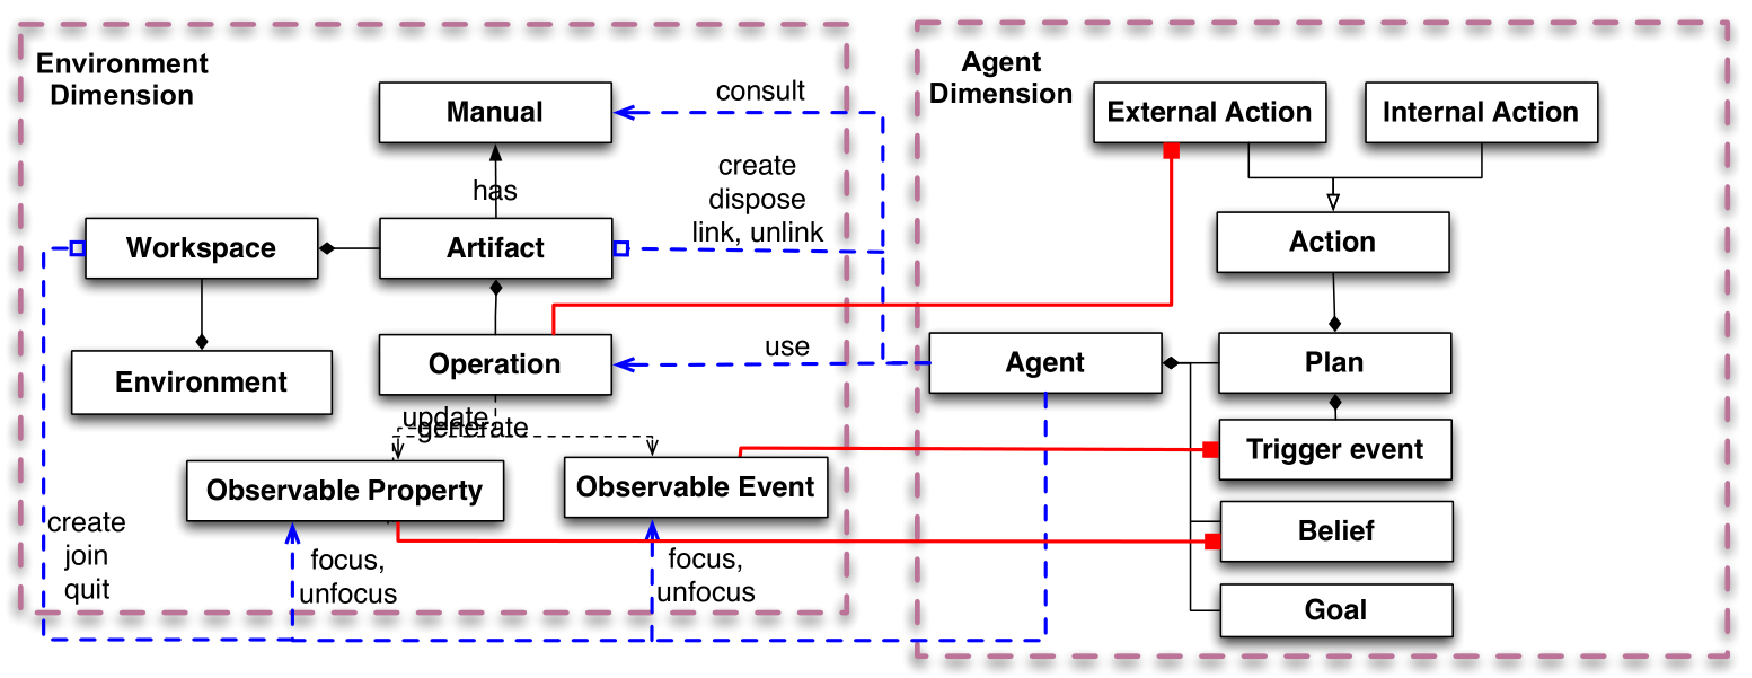
\includegraphics[width=1.2\textwidth]{eps/agent-environment.pdf}}
	\caption{Modello di interazione tra Agenti e Environment.}
	\label{fig:jacamo}
\end{figure}

Avendo JaCaMo il supporto su Java per quanto riguarda la definizione di Artefatti e estensioni per Agenti, per le classi definite in questi ambiti si adotterà il principio della separazione dei componenti, dividendo il \textit{model} e la \textit{view}, ove possibile. È però necessario ricordare che la strutturazione ad Agenti ha una propria visione, in quanto essi possiedono la \quotes{conoscenza} \textit{(belief)}: l'insieme delle cose che sanno e che apprendono. Un artefatto, inoltre, può esporre delle proprietà osservabili all'esterno, rendendo però la loro definizione necessaria all'interno dello scope dell'artefatto stesso.

\subsection{Linguaggi}

\subsubsection{Principali}
Come definito in precedenza, JaCaMo può far uso di Java per la definizione di alcuni suoi elementi. Il linguaggio scelto permette poi la definizione di ulteriori cose, seguendo un classico stile di programmazione.\\

Java possiede molteplici vantaggi, dove tra quelli principali si possono trovare un vasto supporto della community, un'ampia scelta di librerie e la facilità con la quale le applicazioni al giorno di oggi vengono gestite. Diversi aspetti di questo linguaggio però portano a serie considerazioni sul perchè sia ancora uno dei principali utilizzati nell'ambito dello sviluppo. In primo luogo, è estremamente laborioso gestire i tipi opzionali, vi è solo parziale supporto alla null-safety e ogni classe scritta introduce del non banale boilerplate.\\

Per poter soddisfare il requisito per l'uso di tecnologie innovative, Java non pare una soluzione adeguata; dall'altra parte, utilizzando JaCaMo non vi è modo di utilizzare un linguaggio diverso. Per questo motivo si decide di puntare su uno dei linguaggi Java-based tra Scala e Kotlin.\\

Scala risulta essere un linguaggio che punta più sulla programmazione funzionale. Ridefinisce in modo sostanziale quelle che sono le classi e interfacce di Java, ponendole più secondo il suo stile. Per i programmatori non esperti, il linguaggio può sin dall'inizio sembrare più difficile, ma a lungo andare offre funzionalità molto potenti che permettono di abbreviare e semplificare il codice Java. Kotlin risulta essere più una via di mezzo, che non punta ad essere puramente funzionale; esso conserva di più lo stile java-like di classi e interfacce, introducendo soltanto qualche novità. Offre però una gestione di quest'ultime decisamente migliore, nonchè aggiungendo anche la null-safe e l'uso innato di tipi opzionali.\\

Entrambi i linguaggi rimangono compatibili con Java ed entrambi offrono funzionalità non presenti nativamente: essendo però Kotlin più vicino allo stile di Java, si preferisce di non puntare il tutto sul funzionale e rimanere più al livello base, per non incorrere a problemi implementativi, anche a causa della scarsa esperienza con i linguaggi funzionali. Rimanendo quindi JaCaMo perfettamente funzionante, il riferimento per la programmazione \quotes{classica} sarà Kotlin.

\subsubsection{Secondari}
JaCaMo, oltre a Java, utilizza internamente due linguaggi che permettono:
\begin{itemize}
	\item la definizione degli agenti - \textbf{AgentSpeak} (nella versione estesa), interpretata da Jason;
	\item la configurazione dell'ambiente di JaCaMo nel file \textit{.jcm} - \textbf{markup simil-JSON proprietario};
	\item eventualmente, la definizione dell'organizzazione tramite Moise - \textbf{XML}.
\end{itemize}
 
Oltre all'ambiente di JaCaMo, vi è necessità di utilizzare un linguaggio per la definizione della Thing Description: come definito dallo standard W3C \cite{td}, viene utilizzato JSON nella versione \textit{JSON-LD 1.1} \cite{json-ld}, mentre per la definizione delle Thing Status si utilizzerà il formato definito dallo standard RDF.\\

Ulteriori linguaggi verranno presi in considerazione soltanto definendo quali librerie si vorranno utilizzare.


\subsection{Sistema Operativo \& PC}
Il progetto verrà svolto interamente su una macchina con Windows 10, configurata con le seguenti caratteristiche:

\begin{table}[h]
	\centering
	\begin{tabular}{|l|l|}
		\hline
		\textbf{Component}   & \multicolumn{1}{c|}{\textbf{Name}} \\ \hline
		\textbf{Motherboard} & MSI Z270 M7                        \\ \hline
		\textbf{CPU}         & Intel i7-7700k                     \\ \hline
		\textbf{GPU}         & Gigabyte GTX 1080Ti                \\ \hline
		\textbf{RAM}         & Ballistix DDR4 @ 2400MHz           \\ \hline
		\textbf{Disk}        & SSD Samsung Evo Pro 750 1TB                \\ \hline
	\end{tabular}
	\caption{\label{tab:pc-spec} Configurazione del PC sul quale verrà realizzato il progetto.}
\end{table}

\subsection{Librerie \& Tool}
Oltre alla definizione di linguaggi e architettura generale, si vogliono definire in principio alcune delle librerie e tool che verranno utilizzate nel progetto.

\paragraph{Librerie}
\begin{itemize}
	\item \textbf{TornadoFX} \cite{tornadofx} - facilita la creazione delle interfacce utente, utilizzando una sintassi pesantemente basata sull'uso di Kotlin. Facilita la creazione dei layout e l'applicazione dello stile, che a differenza di JavaFX (su cui è basato) non è scritto in \textit{CSS} custom, ma sempre tramite codice Kotlin. Per il suo utilizzo è comunque necessario includere dipendenze di JavaFX.
\end{itemize}
	
\paragraph{Tool}
\begin{itemize}
	\item \textbf{Gradle} \cite{gradle} - facilita la composizione, creazione e la gestione delle dipendenze. È praticamente obbligatorio in qualsiasi progetto con un minimo di complessità non solo per praticità, ma per necessità. Permette la creazione di script per il corretto build delle applicazioni.
	
	\item \textbf{Eclipse} \cite{eclipse} - IDE per la programmazione, che supporta il plugin per lo sviluppo in JaCaMo  \cite{eclipse-j}.
	
	\item \textbf{IntelliJ} \cite{intellij} - IDE per la programmazione, funzionante meglio con il linguaggio Kotlin  \cite{intellij-k}.
	
	\item \textbf{Visual Studio Code} \cite{visualstudiocode} - IDE più leggero e pratico, nel caso di piccole modifiche al volo di parti del codice e/o apertura dei file.
	
	\item \textbf{Git}, \textbf{GitHub}, \textbf{GitHub Desktop} \cite{git} - sistema di versioning, il sito per la gestione del repository e il programma in versione desktop.
\end{itemize}

\subsection{Casi d'uso}
L'architettura deve permettere all'utente di interfacciarsi con tutte le Smart Things tramite un unico terminale. Previa una configurazione, esso deve automaticamente regolarsi in base alle impostazioni dell'utente, che è comunque abilitato a interagire con le singole cose manualmente, sovrascrivendo le eventuali modifiche effettuate dal manager. Seguendo i requisiti, le tre Smart Things e i relativi casi d'uso che si vogliono coprire sono rappresentati nella seguente figura.

\begin{figure}
	\centering
	\makebox[\textwidth][c]{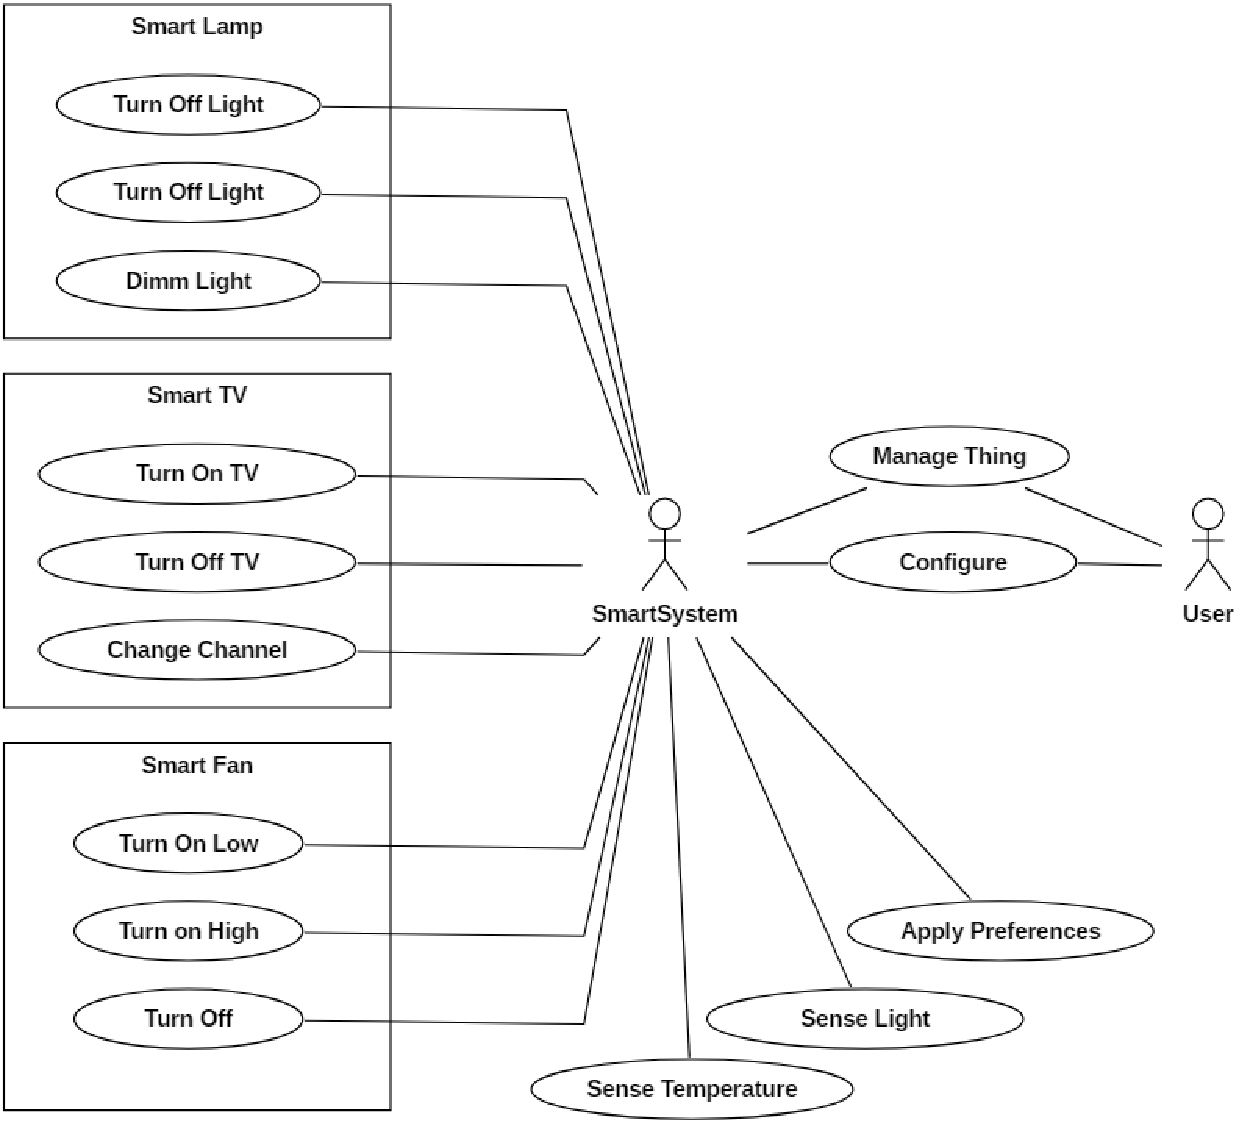
\includegraphics[scale=0.8]{eps/use-case.pdf}}
	\caption{Casi d'uso del sistema in progettazione.}
	\label{fig:use-case}
\end{figure}

\section{Design di Dettaglio}



%%%%%%%%%%%%%%%%%%%%%%%%%%%%%%%%%%%%%%%%%non numera l'ultima pagina sinistra
\clearpage{\pagestyle{empty}\cleardoublepage}
\chapter{Proof of Concept - Realizzazione}           %crea il capitolo
%%%%%%%%%%%%%%%%%%%%%%%%%%%%%%%%%%%%%%%%%imposta l'intestazione di pagina
\lhead[\fancyplain{}{\bfseries\thepage}]{\fancyplain{}{\bfseries\rightmark}}  


%%%%%%%%%%%%%%%%%%%%%%%%%%%%%%%%%%%%%%%%%non numera l'ultima pagina sinistra
\clearpage{\pagestyle{empty}\cleardoublepage}
\chapter{Retrospettiva e commenti}           %crea il capitolo
%%%%%%%%%%%%%%%%%%%%%%%%%%%%%%%%%%%%%%%%%imposta l'intestazione di pagina
\lhead[\fancyplain{}{\bfseries\thepage}]{\fancyplain{}{\bfseries\rightmark}}  

\end{comment}



\begin{comment}
	

\subsection{MVC}
\subsubsection{Model}
Il Model deve rappresentare tutti i concetti necessari a garantire una completa gestione della partita e, più in generale, a soddisfare tutti i requisiti delineati al Capitolo \ref{chapter:Requisiti}. Tale compito è suddiviso nelle seguenti componenti principali.
\begin{itemize}
	\item \textbf{Core.} Si occupa di modellare le entità caratterizzanti il dominio applicativo.
	\item \textbf{Logic.} Gestisce le logiche di relazioni derivanti dalla movimentazione dei pezzi immersi in un ambiente di gioco.
	\item \textbf{History.} Descrive e memorizza le varie situazioni di gioco incontrate nel corso di una partita, occupandosi di classificarle e consentendone la consultazione.
	\item \textbf{Notations.} Parte dell'applicazione incaricata di serializzare opportunamente le azioni di gioco sottopostole in Notazione Algebrica Standardizzata, gestendo anche conversioni in formato FEN.
\end{itemize}

\subsubsection{View}
La componente View ha come obiettivo l'interfacciamento delle funzionalità offerte dall'applicazione all'utente finale, in modo tale da essere completa (dal punto di vista delle feature offerte), semplice (anche gli utenti meno esperti dovranno essere capaci ad usarla) e piacevole (per offrire una bona user experience). La view dovrà rispondere a diversi scenari: la figura \ref{fig:case_uses} riassume le azioni che l'utente potrà compiere dopo aver lanciato l'applicazione.

\subsubsection{Controller}
Il Controller osserva la View e coordina le varie parti del sistema. Nello specifico, possono essergli imputate le seguenti responsabilità:
\begin{itemize}
	\item \textbf{Coordination.} Orchestra l'intera evoluzione della partita, fungendo da intermediario tra le volontà dell'utente e le meccaniche di gioco.
	\item \textbf{Database.} Si occupa di gestire gli aspetti legati alla connessione al db remoto e alla realizzazione del pattern architetturale \textit{DAO}\footnote{Data Access Object.} per la gestione dei dati memorizzati.
	\item \textbf{Scheduling.} Regola gli aspetti di timing richiesti sia dall'orologio doppio che dalla riproduzione automatica dello storico.
	\item \textbf{Settings.} Personalizza l'esperienza di gioco in funzione delle preferenze espresse dall'utente e le opportune configurazioni per le tecnologie utilizzate.
\end{itemize}

\newpage
\begin{landscape}
	\begin{figure}
		\includegraphics[scale=0.35]{eps/3_schema_view.pdf}
		\caption{Diagramma dei casi d'uso della view.}
		\label{fig:case_uses}
	\end{figure}
\end{landscape}
\newpage

\section{Multiplayer}
Per realizzare la componente Multiplayer si è deciso di gestire l'interazione tra le due istanze di gioco tramite scambio di messaggi grazie al paradigma ad attori.

Inizialmente, per avviare la fase di \textit{discovery}, l'approccio è classificabile come \textit{Client-Server}.
\begin{itemize}
	\item \textbf{Creator:} Una volta avviato mette a disposizione le coordinate per poter essere raggiunto da uno sfidante.
	\item \textbf{Challenger:} Invia un messaggio verso il Creator scelto, per notificarlo della volontà di avviare una partita.
\end{itemize}

\begin{figure}[!htb]
	\centering
	\includegraphics[scale=1]{eps/3_actors_arch.pdf}
	\caption{Diagramma di sequenza per la fase di \textit{Discovery} dei due attori.}
\end{figure}

Il lancio della sfida avvia un \textit{Three Way Handshake} che permette ad entrambi gli attori di assicurarsi della presenza l'uno dell'altro, oltre al trasporto di informazioni come la modalità di gioco e la durata della partita in piggyback.

Passata la fase di \textit{Discovery}, gli attori sono entrambi sincronizzati ed è possibile avviare la partita seguendo un vero e proprio approccio \textit{Peer to Peer}, essendo entrambi gli attori considerabli allo stesso livello: entrambi autonomamente inviano e ricevono messaggi.

Unicamente le mosse legali, validate dal client in cui vengono performate, sono poi inviate tramite messaggio all'avversario, che a sua volta cercherà di eseguire la medesima mossa. Nel caso la mossa risulti corretta, sarà possibile procedere con la mossa successiva, altrimenti il ricevente riconoscerà una situazione di \textit{mismatch} e la comunicherà all'avversario, terminando la partita.

Non è previsto alcun meccanismo di recovery, essendo comunque alquanto improbabile il caso in cui avvenga un mismatch essendo entrambi i client in grado di effettuare i medesimi controlli, ma si è comunque deciso per ragioni di sicurezza di introdurre un controllo per evitare che i due client rappresentino due situazioni di partita inconsistenti tra loro.

Qualsiasi arresto anomalo di un client viene intercettato dall'altro, che dichiarerà conclusa la partita.

Successivamente ad una conclusione naturale della partitta (patta o sconfitta di uno dei due giocatori per ragioni di gioco), entrambi i client passano autonomamente in una fase finale per gestire l'eventuale upload della partita su database per poterne poi fruite attraverso la \textit{Modalità TV}. L'attore \textit{Creator} avrà il compito di raccogliere sia la preferenza in arrivo dal proprio client, sia quella in arrivo dall'altro client tramite il rispettivo attore, per poi valutare le condizioni e le modalità dell'upload.

\section{Tecnologie}
\label{sec:Tecnologie}
Nella realizzazione del progetto si è scelto di ricorrere principalmente alle funzionalità offerte dal linguaggio \textit{Scala}, tentando di sfruttare a pieno le sue caratteristiche per il raggiungimento di un massimo beneficio didattico. L'integrazione dei paradigmi \textit{OOP} e \textit{FP} concretizzata dal suddetto linguaggio di programmazione - atta a fonderne i vantaggi - ha infatti concesso un rapido superamento di problemi complessi. Un simile risultato sarebbe stato difficile da replicare con un linguaggio puramente ad oggetti (come \textit{Java}), dove la rigidità del paradigma avrebbe probabilmente comportato sforzi e tempi di sviluppo significativamente più elevati. In questa sezione sono riportate le principali scelte tecnologiche che hanno influenzato lo sviluppo, a fronte di esigenze non coperte nativamente dal linguaggio scelto.

\subsection{JavaFX}
La scelta di un framework ben strutturato e consolidato nel tempo permette di non incorrere in eventuali difficoltà per quanto concerne il raggiungimento di un risultato in termini visivi. È questo il motivo per cui nello sviluppo dell'interfaccia grafica si è voluto usare una tecnologia capace di offrire una ricca documentazione e una soddisfacente quantità di esempi reperibili gratuitamente online, permettendo di evitare problematiche relative alle librerie e/o wrapper privi di una community di supporto attiva.

\subsection{Akka}
Per lo sviluppo della componente \textit{multiplayer} si è utilizzato il modello ad \textit{Attori}, facendo affidamento al toolkit \textit{\textbf{Akka}} per le sue ottime caratteristiche in termini di scalabilità, prestazioni e tolleranza ai guasti. Inoltre, essendo nativamente scritta in \textit{Scala}, tale tecnologia si configura come una scelta naturale per via della sua perfetta integrazione anche con le altre parti del sistema.

\subsection{Scala's Parser Combinators}
All'interno del progetto si è fatto uso della libreria \textit{Scala Standard Parser Combinator}\cite{ScalaParserCombinator} per la ricostruzione di un intero gioco a partire dalla sua rappresentazione in formato PGN.
I \textit{\textbf{Parser Combinator}} costituiscono uno strumento potente per la scrittura di analizzatori lessicali (\textit{lexer}) e \textit{parser} - modulari e componibili - in una idiomatica \textit{Scala}, con un quantitativo di codice ridotto.

\subsection{MongoDB + MongoDB Atlas}
Nello stabilire quale database adottare per la memorizzazione dei dati e la loro interrogazione, si sono considerati anche i diversi possibili sviluppi social che una probabile evoluzione del progetto potrebbe avere in relazione alla modalità TV, le funzionalità multiplayer e l'editing delle PGN. In funzione di questi aspetti e di quelli già emersi durante l'analisi dei requisiti elencati nel precedente Capitolo \ref{chapter:Requisiti}, è apparsa evidente la necessità di adottare una tecnologia capace di gestire frequenti interazioni col database, grandi quantità di dati correlati tra loro, con una struttura potenzialmente complessa e non definibile a priori.


Nonostante il modello relazionale sia comunque in grado di soddisfare l'attuale obiettivo posto col progetto in esame (a causa dell'assenza di stringenti requisiti non-funzionali), si è ritenuto pertanto più saggio - nell'ottica anche di anticipazione del cambiamento - adottare un database di tipo \textit{NoSQL}.


Si è così scelto di ricorrere a \textit{\textbf{MongoDB}}, DBMS non relazionale orientato ai documenti e basato sul formato JSON per la memorizzazione e la rappresentazione dei dati. Tale decisione è ulteriormente giustificata dalla presenza di \textit{\textbf{MongoDB Atlas}}\cite{MongoDBAtlas}: un servizio cloud completamente automatizzato e fruibile attraverso piani gratuiti (soddisfacendo il requisito implementativo legato alle esigenze in termini di costo) - sotto vincoli compatibili con le necessità del sistema - senza l'obbligo di inserimento di dati inerenti una carta di credito, a differenza della maggioranza degli altri provider disponibili e del medesimo livello. \textit{MongoDB Atlas}, nello specifico, è un Database-As-A-Service per \textit{MongoDB}, progettato e gestito dallo stesso team del database. La presenza di un'interfaccia utente e di un'API di facile utilizzo ha inoltre consentito di dedicare più tempo alla creazione del progetto e meno alla gestione del database in quanto tale.
% PARLARE DELLO SCALA DRIVER, DELLA CONFIGURAZIONE E DEGLI ASPETTI DI PRIVACY
\begin{comment}
Subsection with label.\\
Figure citing \ref{fig:dinamica_gameoflife}.\\
Equation:
\begin{equation}
N (compute) + N * (8 (ask neighbors) + 8 (neighbors reply) + 1 (notify grid))
= 18N
\label{eq:NumeroMessaggiSoluzioneSemplice}
\end{equation}



%%%%%%%%%%%%%%%%%%%%%%%%%%%%%%%%%%%%%%%%%non numera l'ultima pagina sinistra
\clearpage{\pagestyle{empty}\cleardoublepage}
\chapter{Design di dettaglio}           %crea il capitolo
\label{chapter:DesignDettaglio}
%%%%%%%%%%%%%%%%%%%%%%%%%%%%%%%%%%%%%%%%%imposta l'intestazione di pagina
\lhead[\fancyplain{}{\bfseries\thepage}]{\fancyplain{}{\bfseries\rightmark}}


- pattern di progettazione
- definizione sistemi per coprire requisiti + interface segregation principle (ISP) + gerarchia interfacce a 3 livelli + nomenclatura per distinzione
- definizione property di 1°, 2° e 3° livello
- definizione entità e rappresentazione delle loro relazioni con le property
- pattern observer e principio DRY
- gestione dei file ed impostazioni: singleton + pattern observer
- view: composizione in scene associate a schermate con cui può interagire + 2 vincoli (solo la View può comunicare direttamente con il Controller E scene limitate ai soli metodi che permettono di soddisfare i requisiti) per aderire a ISP, scene indipendenti le una dalle altre, evitare ripetizioni di codice + realizzazione indipendente dalla libreria grafica utilizzata + navigazione tra scene senza singleton in stile MVVM ma con navigazione controllata + separazione dei pattern architetturali senza controller per Single Responsibility Priniciple (SRP) + dichiarazione interfacce con organizzazione e schema + diagramma sequenza per interazione View, Controller e Model.
- multiplayer: distinzione delle tre macro fasi (lobby con handshaking, inizializzazione con negoziazione informazione, gioco) + diagramma casi d'uso con Server/Client + handshake con pattern Ask e creazione attori temporanei dal framework + diagramma di sequenza per fase di handshaking + gestione lobby + comunicazione durante le fasi di gioco.

- analisi struttura e principali pattern di progettazione adottati
- suddivisione dei servizi: divisione a microservizi
- core (parti riusate dai diversi sottoprogetti): utils, model, services + sotto-progetto solo per semplificare l'esecuzione dei test sui servizi (impliciti e avvio automatico) + diagramma componenti core
- discovery (ciò che consente di fare e tabella con risposte)
- authentication (registrazione, login e verifica token)
- rooms con DAO e Future per chiamate non bloccanti su db relazionale
- client e descrizione schermate di autenticazione, lobby delle stanze e game view
- descrizione elementi di Model
- struttura database
- DAO con le operazioni CRUD
- schema model
- schema strategie

- discussione scelte di design nello sviluppo delle diverse componenti del sistema
- diagramma dei package
- controller (loader e saver + YAML e motivo dell'adozione + dati + builders con pattern funzionale Abstract Types in combinazione con Template Method + uso di impliciti per default values con pattern Type Class in combinazione con Pimp My Library + runner per far fronte a criticità del sistema con aggiornamento continuo della View grazie a flussi di controllo distinti + simulatore + caching + doppia pipeline di gestione + watchers reportistici + salvataggio simulazione con risoluzione di problemi emersi e savable con generici)
- model: spiegazione dominio + dna (elementi costitutivi genoma) con rappresentazione gerarchia trait e classi e spiegazione componenti + gerarchia dei genomi (INTERESSANTE per i nostri controller) + brain con flow chart + decision tree per supporto alle decisioni + memoria + riproduzione ecc.
- view: diagramma di sequenza + isolamento + pattern observer come struttura generale + 3 flussi di comunicazione mediante interfacce + spiegazione delle varie view con interfacce e classi astratte + factory method e pattern strategy

E NOI?
FOCUS SUI PATTERN. Eventualmente component diagram.
- Model
  Spiegare tutte le entità, mostrare schemi gerarchici e di composizione.
  - Game, Board, Piece, Flags, ChessColor, Position (ISP) FATTO
  - Logic
  - History FATTO
  - Pgn
- Controller
  - Scheduling
  - Database + Settings
  - User preferences
  - Controller
- View
  - Scene, View, WindowManager (Singleton in stile MVVM), ...
  - Spiegazione singole scene
  - Diagramma dei casi d'uso
- Come comunicano tra loro
  Diagrammi di sequenza View -> Controller -> Model
\end{comment}

%TODO: guardare pattern usati dagli altri

\begin{comment}
\section{Model}
\subsection{Core}
I principali aspetti del dominio applicativo devono essere modellati e raggruppati all'interno di un package denominato \textit{Core}.

\begin{figure}[!htb]
	\centering
	\includegraphics[scale=0.55]{eps/4_core.pdf}
	\caption{Schema di massima della suddivisione delle classi ad uso della classe principale, \textit{Game}.}
\end{figure}

\subsubsection{Game}
\begin{figure}[!htb]
	\centering
	\includegraphics[scale=0.45]{eps/4_board_game.pdf}
	\caption{Diagramma delle interfacce da implementare per avere uno specifico \textit{BoardGame}.}
\end{figure}
La classe \texttt{ChessGame} è probabilmente quella su cui poggia l'intero progetto, ed è quindi stata rivisitata, aggiornata e modificata più volte da tutti i componenti del team in diverse iterazioni, per supportare costantemente le nuove funzionalità del progetto.

L'istanza di \textit{Game} deve contenere al suo interno tutte le componenti fondamentali del gioco stesso, così da comportarsi come punto di accesso per il \textit{GameController} permettendogli di gestire una partita completa.
Un \textit{BoardGame} contiene tutte le informazioni necessarie per lo svolgimento del gioco.
\begin{itemize}
	\item Riferimento alla board.
	\item Rifermento ai giocatori ed ai relativi colori caratterizzanti.
	\item Riferimento al turno corrente.
	\item Riferimento alla cronistoria degli avvenimenti.
\end{itemize}

Inoltre un \textit{ChessGame} deve permettere la persistenza delle informazioni richieste per lo svolgersi del gioco secondo le regole degli Scacchi.
\begin{itemize}
	\item Riferimento ad eventuali situazioni particolari, in una struttura apposita, per la gestione di:
	\begin{itemize}
		\item Disponibilità di effettaure la mossa Arrocco tenendo traccia di tutte le varianti possibili secondo il regolemtno.
		\begin{itemize}
			\item Re bianco, lato sintro della scacchiera.
			\item Re bianco, lato destro della scacchiera.
			\item Re nero, lato sintro della scacchiera.
			\item Re nero, lato destro della scacchiera.
		\end{itemize}
		\item Disponibilità di effettaure la mossa En-Passant per il giocatore di turno, con annessa casa in cui è possibile performare l'azione.
		\item Disponibilità di effettuare la Promozione per il giocatore di turno.
		\item Numero di mezze mosse effettuate.
		\item Numero di mosse complete effettuate.
	\end{itemize}
	\item Riferimento alla data in cui viene avviata la partita.
\end{itemize}

Oltre alle informazioni di cui un \textit{Game} deve necessariamente tenere traccia, deve offrire anche le funzionalità minime di interazione con esse.
\begin{itemize}
	\item Muovere un pezzo.
	\item Dichiarare la partita conclusa, con annessa motivazione.
	\begin{itemize}
		\item Patta, specificandone la causa.
		\item Sconfitta di uno dei due giocatori, specificandone la causa.
	\end{itemize}
\end{itemize}

Un \textit{ChessGame} deve ulteriormente offrire le funzionalità relative al gioco degli scacchi.
\begin{itemize}
	\item Determinare la situazione di entrambi i Re nella scacchiera.
	\begin{itemize}
		\item Libero.
		\item Sotto Scacco.
		\item Sotto Scacco Matto.
		\item Sotto Stallo.
	\end{itemize}
	\item Calcolare le possibili mosse di ciascun pezzo, data la situazione corrente.
	\item Effettuare una promozione.
	\item Permettere di estrarre ed elencare tutti i pezzi che rispettano determinati criteri, forniti in input.
	\item Valutare se la regola delle cinquanta mosse è applicabile.
\end{itemize}


\subsubsection{Board}
Seguendo la logica usata in più parti del progetto, la ChessBoard implementata estende da un generico trait Board, che richiede l'implementazione delle principali azioni di un qualsiasi gioco basato su una Board, come potrebbe essere ad esempio Dama.

Una Generica Board deve tenere in memoria i pezzi attualmente su di essa, localizzati tramite la relativa posizione, ed un elenco dei pezzi che sono stati rimossi.
Una generica Board inoltre deve essere in grado di gestire le possibili azioni su di essa.
\begin{itemize}
	\item Posizionare un pezzo su di essa, in una posizione valida.
	\item Resettarla secondo le regole stabilite in fase di implementazione.
	\item Permettere la cattura di un pezzo.
	\item Ottenere il riferimento di un pezzo occpante una data posizione, se presente.
	\item Muovere un pezzo da una posizione ad un'altra, secondo i vincoli della Board stessa.
\end{itemize}

Inoltre una \textit{ChessBoard} deve essere in grado di soddisfare le principali richieste per il gioco degli scacchi.
\begin{itemize}
	\item Localizzare le posizioni dei due Re presenti.
	\item Riconoscere il ruolo di un pezzo.
	\item Permettere la promozione di un pezzo, che consiste nel sostituire il pezzo con un altro del medesimo colore ma di un ruolo diverso.
\end{itemize}

\subsubsection{Color}
Si è deciso di utilizzare due case object per modellare i due colori rappresentanti i giocatori di una partita di scacchi, Bianco e Nero, facendoli estendere da un trait comune.

All'interno di ciascun case object vengono implementate le costanti che caratterizzano il colore stesso, come la posizione di partenza dei pedoni o la linea in cui si può effettuare una promozione.

Inoltre è stato definito l'operatore unario ! per permettere di utilizzare la notazione !color all'interno del codice, per ottenere rapidamente l'avversario.

Infine, all'interno di ciascun ChessColor, è salvata una struttura di appoggio per le costanti ed i metodi necessari per la valutazione e l'esecuzione dell'enpassant.

\subsubsection{Piece}
\begin{figure}[!htb]
	\centering
	\includegraphics[scale=0.54]{eps/4_piece.pdf}
	\caption{Rappresentazione della composizione di un \textit{Piece} in relazione alle sue interfacce ed ai due componenti caratterizzanti.}
\end{figure}
Il Pezzo è il componente fondamentale che popola la Board. Si contraddistingue dagli altri grazie alle due componenti che lo formano, \textit{Color} e \textit{Role}.

Grazie alle due componenti, è in grado di calcolare autonomamente tutte le direzioni nella quale è in grado di muoversi, assumento che la board sia vuota.

Oltre a questo, un \textit{ChessPiece} è in grado di assegnare a ciascuna direzione una \textit{ChessPieceQuery} che ne determina il comportamento a fronte dell'incontro con eventuali pezzi in una seconda analisi, ed un'eventuale \textit{ChessPieceSideEffect} nel caso venga riconosciuta la mossa come speciale ed avente un effetto collaterale, anch'essa durante una seconda analisi messa in atto durante la valutazione della mossa all'interno di una Board popolata da altri pezzi nello svolgimento di una partita.

\subsection{Roles}
\label{subsec:Roles}
La progettazione dei ruoli è uno degli elementi cardine su cui si costruisce l'intero progetto in quanto definisce le capacità di movimentazione di tutte le tipologie di pezzi previste dagli scacchi. Durante questa fase di design si è dovuto distinguere tra pezzi con un pattern di movimento dipendente dal colore loro assegnato (re e pedone) e pezzi con un ruolo indipendente da tale aspetto. Si è inoltre dovuto fare distinzione tra i pezzi con un movimento radiale (re e cavallo) e pezzi con movimenti vettoriali.\\
La Figura \ref{fig:roles} sintetizza quanto appena descritto.
\begin{figure}[!htb]
	\label{fig:roles}
	\centering
	\includegraphics[scale=0.54]{eps/4_roles.pdf}
	\caption{Class diagram della strutturazione gerarchica dei ruoli degli scacchi.}
\end{figure}

\subsection{Logic}
Gli aspetti relativi alla logica di movimento e interazione degli elementi del dominio devono rispettare appieno le regole del gioco ed essere raggruppati all'interno di un package denominato \textit{Logic}.

\subsubsection{PathControl}
Il movimento di un pezzo in una determinata direzione deve poter dar luogo ad uno scenario ben definito, nel quale devono essere specificati i confini dello spostamento stesso. Nello specifico:
\begin{itemize}
	\item Deve essere possibile prevedere un limite, escluso il quale, il pezzo in esame non può proseguire nella direzione scelta.
	\item Nel caso in cui la posizione di avanzamento sia consentita, ma al contempo rappresenti l'ultima raggiungibile, deve essere inclusa nel range delle mosse legali.
	\item Se, invece, dalla posizione raggiunta è possibile avanzare, deve essere consentita la prosecuzione della valutazione delle posizioni successive.
\end{itemize}

\subsubsection{PieceQueries}
Ogni pezzo del gioco possiede una logica di movimento particolare che deve essere tenuta in considerazione nel momento in cui si desidera effettuare una mossa con il determinato pezzo. Nello specifico si deve poter analizzare le mosse legali con o senza dipendenza dal colore del pezzo stesso. \\

Deve essere posta attenzione al movimento di pezzi esenti dalla possibilità di realizzare mosse avanzate e, conseguentemente, di quelli che ne sono autorizzati.

\begin{itemize}
	\item Per tutti i pezzi deve essere consentita la possibilità, rispettando la traiettoria consentita, di:
	\begin{itemize}
		\item mangiare un pezzo di colore opposto, nel caso in cui quest'ultimo occupa la posizione di destinazione;
		\item non poter raggiungere ed occupare la posizione di un pezzo dello stesso colore, arrestandosi quindi in quella immediatamente precedente;
		\item proseguire includendo la posizione raggiunta se attualmente non occupata.
	\end{itemize}
	\item Per i soli pedoni devono essere gestiti due particolari spostamenti:
	\begin{itemize}
		\item prosecuzione in avanti, entro il numero di passi consentiti, con eventuale non inclusione se risulta essere occupata o possibilità di prosecuzione in caso contrario;
		\item considerando il colore, spostamento di un solo passo in diagonale con possibilità di catturare un pedone di colore opposto posizionato accanto il pedone in esame (en-passant).
	\end{itemize}
 	\item Per i soli re deve essere gestita la possibilità di movimento di due case, ovvero effettuare un arrocco, allorchè siano presenti le condizioni necessarie stabilite dal gioco.
\end{itemize}

\subsubsection{SideEffects}
Per specifici tipi di pezzi, pedoni e re, e in presenza di condizioni particolari definite dalle regole di gioco, risulta necessario prevedere la realizzazione di mosse o catture conseguenti al raggiungimento di determinate posizioni di arrivo. Nello specifico:
\begin{itemize}
	\item Effettiva cattura di un pedone posizionato accanto al pedone che desidera spostarsi in diagonale se sono in vigore le condizioni di realizzazione di tale effetto.
	\item Spostamento della torre coinvolta nella particolare mossa conosciuta come arrocco.
\end{itemize}

\subsection{History}
\label{subsec:History}
Una parte fondamentale del Model è senz'altro costituita dai vari elementi che concorrono alla definizione di tutte le funzionalità legate alla History.

\subsubsection{Actions}
\label{subsubsec:Actions}
Un aspetto basilare è rappresentato dalla definizione delle azioni che si possono venire a delineare nel corso di una partita e dei loro legami gerarchici. Prima di addentrarsi nella progettazione dettagliata che coinvolge il salvataggio vero e proprio delle situazioni di gioco all'interno dello storico, è preferibile descrivere con chiarezza come si sia modellata questa area del dominio applicativo.\\
All'interno degli scacchi, si può innanzitutto operare una prima distinzione tra azioni di gioco determinanti la fine della partita e azioni che invece non sono conclusive. Nel primo caso, occorre ulteriormente distinguere tra una patta o una vittoria conseguita da parte di uno dei due giocatori. Tra le azioni di gioco non conclusive vi sono tutte le tipologie di mosse contemplate dal regolamento: movimenti, catture, promozioni, en-passant, arrocco. Si può inoltre osservare come ogni forma di cattura da parte di un pezzo determini anche lo spostamento di quest'ultimo. Un ulteriore motivo di distinzione riguarda situazioni di promozione con o senza cattura di un pezzo nella traversa ultima. Infine, occorre evidenziare come ogni mossa legale del gioco possa potenzialmente determinare uno scacco o uno scacco matto nei confronti del re avversario, oppure uno stallo.\\
In Figura \ref{fig:actions} si riporta la rappresentazione della gerarchia dei trait e delle classi, a fronte dell'analisi appena compiuta.

\begin{figure}[!htb]
	\label{fig:actions}
	\centering
	\includegraphics[scale=0.51]{eps/4_actions.pdf}
	\caption{Class diagram illustrante la gerarchia delle azioni classificabili all'interno di una partita di scacchi e le loro principali caratteristiche.}
\end{figure}

Come è possibile constatare, una {\tt ChessAction} costituisce un tipo particolare di azione in un gioco su scacchiera che coinvolge il tipo di pezzi degli scacchi. Il più importante criterio di separazione riguarda la classificazione di {\tt ChessAction} in {\tt ChessEndingAction} (azione di fine partita) e {\tt CheckableAction} (azione di mossa legale cui è associato un particolare stato del re), da cui si diramano i più specifici trait e le effettive classi di implementazione. Ogni {\tt ChessAction} conserva le informazioni necessarie per la sua specifica tipologia. Questo aspetto è di primaria importanza nell'ottica di offrire un supporto di serializzazione su base notazionale, come sarà poi discusso nel successivo paragrafo \ref{subsubsec:Serialization}. A tal scopo si introducono anche le enumerazioni {\tt DrawReason}, {\tt LoseReason} e {\tt KingState}, i cui obiettivi rispecchiano a pieno il nome loro assegnato e i dettagli emergenti dal diagramma. L'uso del pattern \textit{Template Method} unito all'\textit{ereditarietà multipla} supportata da Scala ha pertanto concesso una modellazione chiara e flessibile di uno scenario relativamente articolato.

\subsubsection{Storing}
Questa sezione descrive la struttura dello storico atta a conservare le informazioni delle azioni di gioco accumulate dall'inizio della partita, motivando i suoi elementi costitutivi. La Figura \ref{fig:storing} propone un semplice ma chiarificatorio diagramma per la tematica in oggetto.

\begin{figure}[!htb]
	\label{fig:storing}
	\centering
	\includegraphics[scale=0.7]{eps/4_storing.pdf}
	\caption{Class diagram illustrante la struttura dello storico.}
\end{figure}

Per modellare il concetto di \quotes{istante di gioco} si è deciso di introdurre la classe {\tt ChessGameStep}. Ogni {\tt ChessGameStep} si compone di una {\tt ChessAction} a esso associato e di una {\tt ChessBoard} allo scopo di poter tener traccia dello stato della scacchiera al passo immediatamente successivo a quello dell'applicazione della mossa o dell'azione di fine partita rappresentata dalla {\tt ChessAction} stessa. La decisione legata al mantenimento della board di gioco è stata perseguita anche nell'ottica di non dover svolgere alcun processo deduttivo per poter poi ricostruire la disposizione dei pezzi a fronte di una navigazione (favorendo la comunicazione interna al pattern MVC e seguendo i principi \textit{SOC} e \textit{SRP}). Una {\tt ChessGameHistory} si può pertanto definire come una sequenza ordinata di {\tt ChessGameStep}.

\subsubsection{Serialization}
\label{subsubsec:Serialization}
La gestione completa della serializzazione delle azioni di gioco in formato AN costituisce l'aspetto più complesso per quanto concerne il componente History nella sua interezza. La difficoltà è determinata dalle numerose regole contemplate dalla notazione algebrica - l'unico sistema ammesso dalla FIDE per la registrazione delle mosse da parte dei giocatori. Per spiegare meglio le scelte progettuali intraprese è utile far riferimento al diagramma UML in Figura \ref{fig:serializer}.
\begin{figure}[!htb]
	\label{fig:serializer}
	\centering
	\includegraphics[scale=0.56]{eps/4_serializer.pdf}
	\caption{Class diagram rappresentante i componenti interessati dal modulo notazionale della History.}
\end{figure}
Con l'obiettivo di dividere il software in moduli ad alta riusabilità, si è ritenuto opportuno definire in prima istanza il trait {\tt BoardGameActionSerializer}, rappresentante il \quotes{contratto} comune a tutti i serializzatori di azioni legate a giochi basati su scacchiera. Già da questo primo elemento emerge un aspetto di interesse che si è voluto introdurre per massimizzare sia la flessibilità che il rispetto dell'\textit{SRP}: la progettazione di un componente adibito esclusivamente alla modellazione di tutte le varianti disponibili per la notazione e alla rappresentazione di una specifica configurazione del serializzatore sulla base degli attributi desiderati ({\tt NotationRules}). Questa scelta di design deriva dalla necessità di dover far fronte alle numerose varianti simboliche esistenti per tale notazione (oltre alla Standard più largamente diffusa), abbracciando anche eventuali cambiamenti futuri (principio \textit{AOC}). Dal momento che nel gioco degli scacchi ogni tipologia di azione possiede proprie esigenze traduttorie, si è voluto riunire il comportamento comune - in termini di separazione di logica basata sulla particolare natura di {\tt ChessAction} - all'interno di una classe astratta, adottando il pattern \textit{TemplateMethod}. {\tt ChessGameActionSerializer} possiede così un metodo protetto (dal momento che dall'esterno è richiesta solo la possibilità di poter serializzare una generica {\tt ChessAction}) per ogni classe individuata nella sezione \ref{subsubsec:Actions}, la cui definizione è rimandata alle specifiche implementazioni. La progettazione adottata, quindi, non solo è in grado di gestire tutte le varianti dell'AN ma anche di consentire con semplicità l'inserimento di un supporto per una qualunque altra notazione (es. \textit{Smith}, qui non delineata in quanto non necessaria ai fini dei requsiti).
Specificatamente al serializzatore per notazione algebrica ({\tt AlgebraicNotationGameActionSerializer}), si sono definite le enumerazioni {\tt CaptureNotation}, {\tt CastlingNotation}, {\tt PromotionNotation}, {\tt CheckNotation} e {\tt CheckmateNotation} in modo da consentirne una piena personalizzazione tramite {\tt AlgebraicNotationRules}. Infine, un aspetto che può apparire secondario ma che in realtà è centrale dal punto di vista della ricostruzione del gioco (vedi Sezione \ref{subsec:Pgn}) è quello motivante la presenza del campo {\tt ambiguity} posto all'interno delle {\tt ChessMoveAction}, come osservabile nella precedente Figura \ref{fig:actions}. L'AN richiede infatti la specifica della traversa, della colonna o della notazione \quotes{lunga} capace di disambiguare un contesto di gioco in cui due pezzi dello stesso tipo possono raggiungere la casella di destinazione specificata. Nonostante si fosse volontariamente sorvolato tale dettaglio in precedenza, quindi, la progettazione della componente notazionale della History va a giustificarne la presenza.

\subsection{PGN}
\label{subsec:Pgn}
La notazione Portable Game (abbreviata PGN) è una rappresentazione universale e portabile - diffusa globalmente in ambito digitale - per la registrazione delle partite di scacchi, realizzata per essere facilmente leggibile dall'uomo e comodamente usabile dai software per computer. Un file PGN (indicato con apposita estensione \quotes{.pgn}) consiste sostanzialmente in un file con testo ASCII suddiviso in due sezioni principali:
\begin{enumerate}
	\item \textbf{Tag pair}. Formata da token con l'obiettivo di fornire le informazioni di massima sulla partita.
	\item \textbf{Movetext}. Costituita dalle mosse numerate e descritte in notazione algebrica standardizzata.
\end{enumerate}
Di seguito se ne riporta un esempio.\\
\renewcommand{\ttdefault}{cmtt}
\begin{lstlisting}[basicstyle=\ttfamily\bfseries\small]
[Event "Casual Game"]
[Site "Chess Multiplayer"]
[Date "2018.10.12"]
[White "Giacomo Frisoni"]
[Black "Marcin Pabich"]
[Result "1-0"]
1. a4 a5 2. b4 b5 3. c4 c5 4. d4 d5 5. axb5 cxb4 6. b6 b3 7. b7 b2 8. bxa8=Q bxa1=Q 9. Qxd5 Qxd4 10. Qxd8+ Kxd8 11. c5 Qxd1+ 12. Kxd1 Na6 13. Bh6 Nb4 14. Ke1 Nc2+ 15. Kd2 e5 16. Kd1 Nb4 17. Ke1 Bxc5 18. h4 gxh6 19. e4 Be3 20. Ne2 Nc2+ 21. Kd1 h5 22. Rh2 h6 23. Rh1 Rh7 24. Rh2 Rg7 25. Rh1 Rg3 26. Rh2 Bg5 27. Rh1 Nb4 28. Ke1 Rd3 29. Rh2 Nc2# 0-1
\end{lstlisting}
\vspace{5mm}
Ai fini del soddisfacimento dei requisiti emersi durante l'intervista col committente (riportati nel precedente Capitolo \ref{chapter:Requisiti}), appare evidente il fatto che debba essere prevista una componente del Model dedita alla conversione di una {\tt ChessGameHistory} o più in generale di un {\tt ChessGame} nella descrizione testuale richiesta dalla notazione in esame. In correlazione con tale problematica, durante lo svolgimento dello studio di fattibilità, ci si è anche interrogati sul come gestire il salvataggio delle partite remote effettuate (operazione richiesta dalla modalità TV). Nel valutare le varie possibili soluzioni, si è ritenuta ottimale la decisione progettuale incentrata sull'uso della PGN anche a tale scopo. Numerosi sono infatti i programmi informatici oggi esistenti capaci di leggere ed elaborare tale rappresentazione di gioco. Perseguire l'obiettivo posto col cliente adottando un approccio di questo tipo consente dunque di aprirsi anche a possibili ulteriori sviluppi, senza che questi possano richiedere grandi sforzi ingegneristici. Come effetto di tale scelta, si necessita che la componente modellistica citata in precedenza sia anche in grado di gestire il \textit{parsing} in notazione Portable Game, oltre che la semplice traduzione di un gioco in formato stringa. In Figura \ref{fig:pgn} è presentato il design derivante da tali sforzi.

\newpage
\begin{landscape}
	\begin{figure}
		\label{fig:pgn}
		\includegraphics[scale=0.7]{eps/4_pgn.pdf}
		\caption{Class diagram relativo alla PGN.}
	\end{figure}
\end{landscape}
\newpage

Il trait {\tt PgnTag} rappresenta uno specifico token PGN di prima sezione. Esso è caratterizzato da due attributi principali: il tipo identificatorio e il valore a esso associato. Durante lo studio di design si è ritenuto necessario dotare {\tt PgnTagType}, oltre che di un nome, anche di un controllo di formato opzionale (validazione infatti richiesta da determinati tipi). Il trait {\tt PgnTags} va invece a modellare una collezione custom di {\tt PgnTag}. Dal momento che la notazione prevede un ordinamento specifico dei token a livello di formato di esportazione (\textit{Seven Roster Tags Rule}), si è tenuto conto sin dalla fase di progettazione di un metodo {\tt sorted} all'interno di {\tt PgnTags} stesso. Il trait {\tt PgnMoves}, infine, modella una mossa legale svolta all'interno della partita (caratterizzata da una descrizione SAN e da una sequenza di eventuali commenti - altra possibilità contemplata dalla rappresentazione).
L'object {\tt PgnConverter} costituisce la \textit{singleton} incaricata di fornire i metodi di pubblica utilità per quanto concerne le operazioni di conversione da {\tt ChessGameHistory} o {\tt ChessGame} a PGN e da PGN a {\tt ChessGame}. Nel successivo elenco si distinguono e si descrivono nel dettaglio i due casi.
\begin{itemize}
	\item \textbf{Da ChessGame a PGN.} Lo svolgimento di questa operazione richiede semplicemente l'utilizzo dell'{\tt AlgebraicNotationGameActionSerializer} descritto nella precedente sezione \ref{subsubsec:Serialization}, avendo l'accortezza di utilizzare una configurazione di regole che rispecchi la simbolica SAN.
	\item \textbf{Da PGN a ChessGame.} È l'operazione più complessa e richiede l'adozione della tecnologia \textit{Scala Parser Combinator}, ritenuta la più idonea durante lo studio architetturale (come già osservato nel Capitolo \ref{chapter:Architettura}). In riferimento al più volte citato \textit{SOC}, si è deciso di separare il macro-problema in più moduli con uno specifico obiettivo (\textit{SRP}).
	\begin{itemize}
		\item {\tt PgnsTagsParser}. Rappresenta il lexer e il parser capace di convertire la prima sezione di una stringa PGN in un oggetto \textit{PgnTags}.
		\item {\tt PgnMovesParser}. Rappresenta il lexer e il parser per la conversione della seconda sezione di una stringa PGN in un elenco di \textit{PgnMove}, fornendo gli eventuali commenti e il risultato della partita ove indicato.
		\item {\tt PgnMoveParser.} Componente capace di calcolare lo stato di gioco successivo, a partire da una mossa espressa in forma testuale SAN e il gioco corrente. Si occupa pertanto di interpretare la SAN e applicare l'azione associata sul {\tt ChessGame} fornito, segnalando eventuali inconsistenze.
	\end{itemize}
	Il metodo \textit{fromPgn} deve pertanto coordinare le chiamate agli object esaminati, gestendo opportunamente tutte le casistiche che si possono venire a presentare. Potendo richiedere potenzialmente diverso tempo per il suo completamento, si è tenuto conto anche dell'uso di \textit{Future} per indicare un valore non \quotes{correntemente} disponibile. Un ulteriore aspetto che si è voluto introdurre sotto questo punto di vista si riferisce alla possibilità di specificare opzionalmente un {\tt FromPgnObserver} come parametro al metodo in esame, in modo da consentire l'invio di notifiche atte a segnalare lo stato di avanzamanto del processo di conversione a chi interessato. Per il raggiungimento di questo obiettivo si è fatto uso del pattern \textit{Observer}.
\end{itemize}


\section{Controller}

\subsection{Scheduling}
\label{subsec:Scheduling}
La gestione degi aspetti temporali ricopre un ruolo di primo piano all'interno di una partita di scacchi disputata utilizzando un orologio doppio e di conseguenza va a rappresentare una componente cruciale del Controller.
La Figura \ref{fig:scheduling} offre una visione complessiva del modulo in esame.
\begin{figure}[!htb]
	\label{fig:scheduling}
	\centering
	\includegraphics[scale=0.54]{eps/4_scheduling.pdf}
	\caption{Class diagram documentante i principali elementi del Controller che concorrono alla gestione dello scheduling.}
\end{figure}
Il trait {\tt ChessClock} rappresenta fedelmente il reale oggetto del dominio applicativo e, a fronte di una specifica iniziale dei valori di partenza legati ai timer di entrambi i giocatori ({\tt startingTimers}), mette a disposizione funzionalità per l'avvio e l'interruzione dell'orologio, nonchè l'emulazione del cambio turno determinato dalla pressione del pulsante da parte del giocatore che lo ha appena concluso. Tale pressione ({\tt whitePressure} o {\tt blackPressure} in funzione di quale giocatore abbia portato a termine la mossa) determina l'arresto del proprio timer e la messa in moto di quello avversario. Nella progettazione del {\tt ChessClock} si è voluto estrarre il criterio di aggiornamento dei singoli timer, facendo uso del pattern \textit{Strategy}. Un {\tt ChessClockStrategy}, nello specifico, definisce i nuovi valori dei timer a fronte di eventi di \quotes{tick} e di \quotes{switch}. Questa scelta di design ha consentito dunque una gestione agevole di tutte le varianti determinate dalle modalità di gioco supportate, come osservabile dal diagramma. Infine si è scelto di ricorrere al pattern \textit{Observer} per la segnalazione di eventi di \quotes{tick} e di \quotes{timeout}.

\subsection{Controller di scena}
Il componente architetturale in esame è stato oggetto di un'approfondita analisi dalla quale è scaturita l'architettura gerarchica che lo caratterizza. In particolare, come già evidenziato all'interno della sezione relativa alla View, ogni specifico controller aderisce ad un Observer. In tale maniera viene quindi veicolata la corretta gestione degli eventi intercettati lato view.

\subsubsection{Struttura gerarchica}
Ogni controller definito all'interno dell'applicazione rispetta una particolare gerarchia. Nello specifico, alla base di essa si trova \textbf{\textit{GenericController[V]}}, il cui compito principale consiste nell'identificare il collegamento diretto tra il controller definito e la relativa \textit{Scene} lato view. In questo modo il controller è in grado di coordinare facilmente la gestione delle chiamate al componente view.\\

In generale, al fine di facilitare la comprensione delle specializzazioni necessarie, si è stata adottata una nomenclatura del tipo \textit{xxx\textbf{SceneController}} per individuare il comportamento relativo al controller definito per quella determinata scena, il quale aderisce allo specifico \textit{xxx\textbf{Observer}}.

\subsubsection{Tipologie}
Al fine di perseguire il principio di \textit{single responsibility} sono stati definiti Observer per ogni diversa categoria di interazione e, per questo motivo anche relativi specifici Controller.

\begin{itemize}
	\item \textbf{\textit{MainSceneController}} è avviato unitamente all'applicazione stessa e si occupa principalmente di gestire il corretto passaggio tra diverse \textit{Scene} dichiarandone l'intento. 
	
	\item \textbf{\textit{LocalGameCreatorSceneController}} l'obiettivo principale è quello di avviare una partita in locale, istanziandola con tutti i parametri necessari reperibili dalla view relativa.
	
	\item \textbf{\textit{MultiPlayerGameCreatorSceneController}} come da nomenclatura, si occupa dell'istanzazione di una partita in remoto, suddividendo quindi le tipologie di giocatori che vi stanno interagendo, al fine di ritrarre tutto il necessario allo svolgimento globale di una partita.
	
	\item \textbf{\textit{SettingsSceneController}} si occupa di gestire le preferenze relative all'abilitazione dell'highlight, all'evidenziazione dell'ultima mossa effettuata e alla visualizzazione o meno delle coordinate della borad di gioco.
	
	\item \textbf{\textit{TvSceneController}} viene avviato per gestire tutte le interazioni necessarie alla corretta esecuzione e fruizione della modalità tv. Si occupa quindi anche di eseguire le opportune operazioni sul database al fine di fruire dei risultati desiderati.
\end{itemize}

\subsubsection{Interazioni di gioco}
Una nota particolare deve essere fatta per quanto riguarda il controller di gioco. \textbf{\textit{GameSceneController}} rappresenta la radice dalla quale sono state successivamente introdotte \textbf{\textit{NormalSceneController}} e \textbf{\textit{TvGameSceneController}}. Alla base di questa decisione vi è la volontà di distinguere le funzionalità fruibili attraverso la stessa schermata a seconda che si tratti di un partita in corso o di una sua riproduzione, in seguito al relativo download da database. Infatti, le funzionalità principali e comuni ad entrambe le modalità sono:

\begin{itemize}
	\item Visualizzazione della board di gioco relativa allo stato di gioco correntemente osservato.
	\item Aggiornamento di pari passo alla board visualizzata dei pezzi mangiati.
	\item Possibilità di navigare la history di gioco, sua riproduzione ed eventuale arresto.
\end{itemize}
L'ultimo punto descritto rappresenta appieno la funzionalità principale della modalità tv, e quindi può essere considerato alla base della scelta intrapresa.\\

La principale differenza tra quanto appena descritto consiste nella presenza o meno dell'orologio doppio su cui una partita in corso necessita di basarsi per il suo corretto proseguimento. 
In merito a ciò, ed in particolare anche per una corretta progettazione della modalità multiplayer, l'interfaccia \textbf{\textit{GameSceneController}} è stata implementata da una classe astratta, \textbf{\textit{AbstractGameSceneController}}. Le conseguenti implementazioni sono quindi state incluse in:

\begin{itemize}
	\item \textbf{\textit{NormalGameSceneController}} rappresentante il controller di base di una partita in locale, il cui compito principale è quello di gestire tutte le interazioni lato model, come il riflettere una mossa eseguita all'interno della board di gioco, e view, per la corretta visualizzazione dello stato corrente.
	\item \textbf{\textit{TvGameSceneController}} adatta il controller affinchè possano essere soddisfatte solo determinate interazioni, ovvero impedendo la possibilità di interagire con la board stessa, perseguendo quindi le mere finalità della modalità tv, ovvero riproduzione di una partita ed eventuale navigazione delle mosse che l'hanno caratterizzata.
\end{itemize}

Ad un secondo livello di dettaglio, a partire da \textbf{\textit{NormalGameSceneController}}, vi è \textbf{\textit{MultiplayerGameSceneController}} il quale, pur dovendo gestire le interazioni all'interno di una partita allo stesso livello di un controller di una partita in locale, necessita di modificarne in parte l'esecuzione per conformarsi alla diversa modalità di gioco. 

\subsection{Attori}
\begin{figure}[!htb]
	\centering
	\includegraphics[scale=0.60]{eps/5_actors.pdf}
	\caption{Gerarchia delle due tipologie di attori.}
\end{figure}
Per l'implementazione degli attori il primo step è quello di individuarne la parte comune, ossia il comportamento durante la partita. Essendo tale comportamento identico, o meglio simmetrico durante l'esecuzione, si è deciso di estrarne tale caratteristica ed implementarla in una classe astratta da cui far estendere entrambi gli attori.

Secondo il pattern template invece, i due metodi astratti {\tt initialBehaviour} ed {\tt finalBehaviour} sono stati dichiarati ed implementati dai due attori. Nella situazione così configurata, la classe astratta è in grado di decidere quando e come passare ai due \textit{Behaviour} caratterizzanti, lasciandone l'implementazione agli attori stessi.

\section{View}

\subsection{Composizione}
\label{sec:view_composition}

Una qualsiasi view è composta da elementi base, chiamati da ora in poi componenti (\textit{Component}).
Un \textbf{\textit{Component}} è una parte della view che si occupa di visualizzare e gestire una determinata categoria di compiti, correlati logicamente tra di loro, attraverso i quali un utente può capire l'attuale stato dell'applicazione ed interagire con essa. I \textit{Component} possono contenere altri \textit{Component} al loro interno, e devono essere visualizzati attraverso delle \textit{Scene}.\\

Una \textbf{\textit{Scene}} è un grande \textit{Component}, che può ospitare al suo interno ulteriori \textit{Component}, che collaborano tra di loro. L'insieme di questi componenti permette di visualizzare a video ogni informazione necessaria alla comprensione di quello che sta accadendo sotto e facilita all'utente la scelta della prossima azione da svolgere. Per permettere alle \textit{Scene} di essere visualizzate, occorre un ulteriore componente, gestente tutti gli aspetti che può avere un contenitore di Scene: una \textit{GenericWindow}.\\

Una \textbf{\textit{GenericWindow}} offre non solo la possibilità di visualizzare una \textit{Scene} al suo interno, ma di gestire ogni aspetto che potrebbe avere una generica finestra di una applicazione, indipendentemente da come verrà successivamente implementata. Inoltre, in caso di necessità e per permettere una migliore User Experience, questa si preoccupa di tutti gli aspetti legati ad eventuali messaggi e notifiche che devono essere visualizzate all'utente. Di conseguenza, ogni \textit{Scene} ha il riferimento alla \textit{GenericWindow} che le gestisce, per permettere il richiamo delle funzionalità richieste.\\

Per facilitare l'individuazione dei componenti, si sceglie di imporre loro dei vincoli sul nome:
\begin{itemize}
	\item il nome \textit{xxx\textbf{Scene}} individua tutte le \textit{Scene},
	\item il nome \textit{xxx\textbf{View}} individua tutti gli altri componenti, che non sono delle \textit{Scene} e che quindo non possono essere usati direttamente in un \textit{GenericWindow}, ma dovranno essere contenuti dentro una \textit{Scene}.
\end{itemize}



\subsection{Navigazione}
La navigazione tra le scene avviene attraverso degli \textbf{\textit{Intent}}: ogni \textit{Scene}, avendo accesso alla \textit{GenericWindow}, può evocare l'apertura di un'altra scena, specificando l'intento alla \textit{GenericWindow}. Quando una particolare scena ha bisogno di determinati dati, l'\textit{Intent} contiene anche le corrispettive informazioni.



\subsection{Tipi di Scene}
\label{sec:Scenes}
L'applicazione deve rispondere a diversi scenari e per rispettare il Single Responsibility Principle vengono predisposte diverse \textit{Scene}.\\

\textbf{\textit{GenericScene}} è la base di tutte le \textit{Scene}. Non è un vero e proprio componente, in quanto è soltanto un'interfaccia che al suo interno prevede l'impostazione di un \textit{GenericWindow}, così ogni componente che ne deriva sarà automaticamente una \textit{Scene} con un riferimento ad una \textit{GenericWindow}.\\

\textbf{\textit{MainScene}} è la scena principale, che appare dopo l'avvio dell'applicazione. In essa si trovano componenti responsabili a portare l'utente su ulteriori scene, che svolgono ruoli più particolari, come ad esempio il creare una partita o il gestire delle impostazioni.\\

\textbf{\textit{LocalGameCreatorScene}} è la scena nella quale l'utente è abilitato a creare una partita locale, scegliendo la modalità di gioco, il tempo, e i nomi di entrambi i giocatori. Da questa l'utente potrà anche tornare indietro nella scena principale.\\

\textbf{\textit{MultiplayerGameCreatorScene}} simile alla precedente, ma con un ruolo diverso, permette di creare una partita multiplayer, facendo scegliere all'utente se essere il creatore della partita o lo sfidante, che si collegherà ad una partita già creata. Il creatore ha la possibilità di decidere tutti i dettagli del gioco (compreso il suo nome), lo sfidante può decidere soltanto il proprio nome.\\

\textbf{\textit{GameScene}} è la scena del gioco vero e proprio. Rappresenta il tavolo sul quale i giocatori (in locale o multiplayer) si stanno sfidando. Essendo una scena complessa, viene suddivisa in due macro-componenti, \textbf{\textit{BoardView}} e \textbf{\textit{DetailsView}}, ognuno incaricato di gestire una parte significativa della scena. Avendo come scopo la visualizzazione del gioco, può essere opportunamente configurata per funzionare in due modalità differenti: sola visione e interattiva.\\

\textbf{\textit{TvScene}} è la scena che permette di visionare tutti i giochi salvati in precedenza; selezionando uno di essi, questo viene aperto in una \textit{GameScene} abilitata alla sola visualizzazione.\\

\textbf{\textit{SettingsScene}} permette all'utente di esprimere le proprie preferenze riguardanti l'applicazione e/o il gioco.\\



\subsection{Altri componenti}
Oltre alle scene sono presenti ulteriori componenti che facilitano la scomposizione delle responsabilità di una Scena (o di un componente complesso).\\

\textbf{\textit{BoardView}} è un componente che permette di gestire la scacchiera, quindi tutte le azioni che si possono compiere all'interno di essa, come ad esempio movimenti e catture. Essendo suddivisa in quadrati della stessa dimensione che svolgono perlopiù lo stesso compito, a sua volta è composta da tanti \textbf{\textit{SquareView}}, quanti serviranno per la sua completa composizione.\\

\textbf{\textit{SquareView}} è un componente piccolo, facente parte di una \textit{BoardView}. Rappresenta la casella con un colore, una posizione ed eventualmente un pezzo al suo interno.\\

\textbf{\textit{DetailsView}} è un componente che gestisce tutti gli aspetti non direttamente collegati al gioco degli scacchi, ma all'applicazione in uso: abilita, ovvero, una serie di funzionalità non presenti durante una classica partita. In questo componente sono disponibili tutti i controlli che permettono la visualizzazione dei giocatori (e dei loro dettagli, quali timer e pezzi mangiati), un componente per la visualizzazione e navigazione della history del gioco e un'altro per gestire le varie richieste dei giocatori (come richiesta della patta). In base alla modalità del gioco scelta (locale / multiplayer) questo componente assume anche il ruolo di coordinazione durante la fase di accoppiamento tra il creatore della partita e lo sfidante.\\




\subsection{ObservableView e ViewObserver}
\label{sec:Observable}
Per catturare gli eventi che possono capitare all'interno della view si è scelto di utilizzare il pattern Observer: nasce il concetto di \textbf{\textit{ObservableView}}, che diventa la base per tutti i generatori di eventi, a partire da una schermata. Un \textit{ObservableView} dunque non fa parte della famiglia dei componenti, ma è un'interfaccia attraverso la quale si specifica che un componente può essere osservato da uno o più \textbf{\textit{ViewObserver}}. Ogni evento scaturito in una qualsiasi parte della view verrà quindi notificato a tutti gli \textit{ViewObserver}, che in quel momento sono registrati tramite l'interfaccia: un \textit{ViewObserver}, quindi, deve poter rispondere a tutti i possibili eventi dichiarati da un particolare componente. Esisterà dunque un tipo di \textit{ViewObserver} per ogni tipo di \textit{ObservableView}.

\newpage
\begin{figure}[!htb]
	\centering
	\includegraphics[scale=0.45]{eps/4_observers.pdf}
	\caption{Vari tipi di observers e la loro organizzazione. Nello schema sono state omesse, per semplicità, tutte le indicazioni degli stereotipi, in quanto tutti gli elementi visibili sono delle interfacce.}
\end{figure}

\newpage
\begin{figure}[!htb]
	\centering
	\includegraphics[scale=0.38]{eps/4_scenes_views.pdf}
	\caption{Composizione delle scene e view. Nello schema sono state omesse, per semplicità, tutte le indicazioni degli stereotipi, in quanto tutti gli elementi visibili sono delle interfacce.}
\end{figure}
\newpage

\chapter{Implementazione}                %crea il capitolo
%%%%%%%%%%%%%%%%%%%%%%%%%%%%%%%%%%%%%%%%%imposta l'intestazione di pagina
\lhead[\fancyplain{}{\bfseries\thepage}]{\fancyplain{}{\bfseries\rightmark}}
In questo capitolo sono analizzati nel dettaglio i contributi apportati da ciascun componente del gruppo.
\section{Pair Programming}
Nella fase iniziale del progetto, gli studenti Giacomo Frisoni, Leonardo Montini e Sofia Rossi hanno lavorato in \textit{Pair Programming} sulle prime versioni di:
\begin{itemize}
	\item {\tt Position} [Frisoni]
	\item {\tt Color} [Montini]
	\item {\tt Role} [Montini]
	\item {\tt Piece} [Montini]
	\item {\tt Board} [Montini]
	\item {\tt Game} [Rossi]
	\item {\tt PieceQueries} [Montini]
	\item {\tt SideEffects} [Rossi]
\end{itemize}
\newpage
\section{Giacomo Frisoni}
All'interno del progetto \textit{Chess Multiplayer} lo studente Giacomo Frisoni si è occupato dello sviluppo delle seguenti parti:
\begin{itemize}
	\item \textbf{Generale}
	\begin{itemize}
		\item Creazione e configurazione del repository Git e del progetto Gradle.
		\item Configurazione di Trello.
	\end{itemize}
	\item \textbf{Model}
	\begin{itemize}
		\item Modellazione del concetto di posizione su una board di gioco, con gestione dei movimenti vettoriali e radiali\\(package {\tt it.unibo.chess.model.core.position}).
		\item Progettazione e implementazione della history con supporto alla serializzazione SAN (package {\tt it.unibo.chess.model.history}).
		\item Riorganizzazione della componente {\tt core} del progetto (a partire dal lavoro di Montini e Rossi) per una gestione più efficace di trait, classi astratte e companion object.
		\item Progettazione e implementazione del parser PGN e dell'operazione di conversione di un {\tt ChessGame} in tale formato (package {\tt it.unibo.chess.model.pgn}).
	\end{itemize}
	\item \textbf{Controller}
	\begin{itemize}
		\item Implementazione di {\tt ChessClock} e gestione del tempo legato ai turni dei giocatori\\({\tt it.unibo.chess.controller.utilities.SchedulingUtilities} e package {\tt it.unibo.chess.controller.scheduling} - ad eccezione della successiva parte svolta da Montini relativamente una logica temporale basata su clock rate).
		\item Sviluppo del controller di gioco per la modalità SinglePlayer, su cui si poggiano le implementazioni di {\tt NormalGameSceneController} e {\tt TvGameSceneController}.
		\item Gestione del database (package {\tt it.unibo.chess.controller.database}).
		\item Salvataggio della PGN su file.
		\item Gestione delle impostazioni su Config legate all'applicazione (package {\tt it.unibo.chess.controller.settings}).
		\item Implementazione del salvataggio delle preferenze utente (package {\tt it.unibo.chess.controller.preferences}).
	\end{itemize}
\end{itemize}
Ha inoltre collaborato con Pabich in merito alle scelte architetturali alla base della View e al design dell'interazione Controller-View.
\subsection{Generale}
Il perseguimento del primo Sprint ha richiesto la preparazione degli strumenti e delle tecnologie necessarie per uno sviluppo del progetto basato su un framework \textit{Scrum-like}.
Mi sono pertanto occupato - in qualità di Product Owner - della gestione del repository Git remoto su Bitbucket, incaricandomi della sua creazione e della configurazione iniziale di \textit{Checkstyle}, \textit{FindBugs}, \textit{PMD} e \textit{Scoverage} nel progetto Gradle. Come già descritto nella Sezione \ref{sec:Metodologia}, sono inoltre stato responsabile delle release di fine Sprint. Ho poi creato la bacheca \textit{Trello} - utilizzata dal team per la pianificazione del lavoro e il tracciamento dei progressi - che ho configurato col Power-Up \textit{Bitbucket Cloud} in modo da poter allegare i commit realizzati dai vari membri alle singole schede.
\subsection{Model}
\subsubsection{Position}
Nello svolgimento del mio lavoro ho sempre cercato di prestare particolare attenzione al principio di \textit{generalità} dell'ingegneria del software, tentando di individuare un buon equilibrio tra le precise funzionalità richieste dall'applicazione e la risoluzione di un problema con una veduta più ampia che potesse promuovere il riuso. Una traduzione di questa volontà è senz'altro rappresentata dalla mia modellazione del concetto di \textit{Posizione}, elemento centrale all'interno del progetto. Trattandosi di un'entità fondamentale nella maggior parte dei giochi da tavolo e non solo, ho preferito adottare un approccio incrementale incentrato sulla costruzione di più \quotes{zone fredde} del codice (non sensibili a variazioni), anzichè sviluppare in modo diretto una soluzione ad hoc che rispondesse alle sole esigenze del contesto applicativo. Ho dunque iniziato dalla definizione di un trait generico {\tt Position}, caratterizzato da una coppia di coordinate riga-colonna e delineante funzionalità di diffuso interesse. Nel far ciò ho adottato il pattern funzionale \textbf{DSL} con l'intento di favorire l'utilizzo di tali API. Sono poi passato alla realizzazione della classe astratta {\tt GridPosition}, rappresentante una posizione su una griglia illimitata. Ho così fornito una prima implementazione dei metodi individuati in precedenza e, allo scopo di restituire nelle varie chiamate uno specifico tipo di {\tt Position}, ho fatto ricorso al pattern \textbf{Template Method} - demandando alle singole implementazioni la definizione di un'operazione di \textit{factory}. Mi sono poi concentrato sulla modellazione di una posizione limitata, introducendo il trait {\tt LimitedPosition} e il concetto di \quotes{validazione} al fine di poter imporre vincoli nel movimento. Sfruttando l'ereditarietà multipla supportata da \textit{Scala}, sono infine giunto alla implementazione della classe {\tt BoardPosition}. Essa modella una posizione su una board quadrata di specifiche dimensioni (ovvero una griglia limitata), accorpando in sè {\tt GridPosition} e {\tt LimitedPosition} con un criterio di validazione incentrato sull'accettazione delle sole posizioni appartenenti al range di coordinate coperto dalla board stessa (vedi Figura \ref{fig:position}). 
Infine, occorre osservare come in quest'ultima fase si sia impiegato anche il pattern \textbf{Strategy} per la specifica dinamica delle dimensioni della griglia. In seguito, ci si è concentrati sulla realizzazione di un object che fornisse le opportune factory per gli scacchi e funzioni di utilità per quanto concerne movimenti vettoriali e radiali. Al fine di migliorare la qualità del codice si è fatto largo uso di \textit{pattern matching} e funzioni ricorsive, portando così il codice in esame a costituire una solida base per il resto del progetto e un interessante esempio didattico, anche per via di un attento uso di generici e all'inserimento di vincoli relativi al tipo.
\begin{figure}[!htb]
	\label{fig:position}
	\centering
	\includegraphics[scale=0.80]{eps/5_position.pdf}
	\caption{Class diagram evidenziante i pattern di programmazione utilizzati per BoardPosition.}
\end{figure}
% TODO: code example

\subsubsection{History}
A causa dei numerosi requisiti che ne domandano la presenza, il componente legato alla \textit{History} ricopre senz'altro un ruolo significativo all'interno del Model. Mi sono occupato sia della sua progettazione (già descritta nella Sezione \ref{subsec:History}) che della sua effettiva implementazione. A seguito di alcune scelte emerse durante lo sviluppo, sono giunto alla soluzione descritta dal diagramma in Figura \ref{fig:detailedHistory}.
Sempre in considerazione dei principi di \textit{generalizzazione}, \textit{riuso} e \textit{modularità}, ho deciso di separare le esigenze comuni a tutti i serializer di azioni derivanti da giochi \quotes{board-based} da quelle dello specifico dominio degli scacchi. A tal fine sono stati inseriti i trait {\tt BoardGameStep} e {\tt BoardGameHistory}, tentando di adottare un sapiente uso di generici. Da essi sono poi derivati i trait \textit{ChessGameStep} e \textit{ChessGameHistory} con le rispettive implementazioni. Sia in questa circostanza che in tutte le altre citate all'interno di questo capitolo, si è prestata molta attenzione nell'esporre esclusivamente il trait a livello pubblico e non direttamente la classe di implementazione (in modo da costringere un passaggio obbligato alle factory di un \textit{companion object}, con l'obiettivo di avere un unico punto all'interno del progetto incaricato della creazione degli oggetti effettivi).\\
In questa fase si è anche dovuto affrontare il problema legato all'esportazione in formato \textit{Json} dello storico. Dopo approfondite ricerche si è scelto di adottare la libreria \textbf{lift-json} del framework \textit{Lift} (una delle più diffuse all'interno dei progetti \textit{Scala}). Questa decisione è da ricondurre al suo noto supporto per le collezioni messe a disposizione dal linguaggio \textit{Scala} stesso, a differenza di altre (come Gson) che - essendo destinate nativamente a \textit{Java} - non sono in grado di offrire una gestione completa necessaria per rispondere alle esigenze di \textit{ChessMultiplayer}.\\
Mi sono inoltre occupato del caricamento delle azioni all'interno della History in {\tt ChessGame}.
\newpage
\begin{landscape}
	\begin{figure}
		\label{fig:detailedHistory}
		\includegraphics[scale=0.70]{eps/5_history.pdf}
		\caption{Class diagram illustrante le scelte fondamentali adottate durante lo sviluppo di ChessGameHistory.}
	\end{figure}
\end{landscape}
\newpage


\subsubsection{Core}
All'interno della componente \textit{core} del Model, mi sono principalmente occupato di una riorganizzazione del codice che non mutasse il principale lavoro già svolto in precedenza da Montini e Rossi. I tre punti di intervento sono di seguito descritti.
\begin{itemize}
	\item \textit{Roles}. Inserimento dei trait e delle classi astratte presentate nella Sezione \ref{subsec:Roles}.
	\item \textit{Piece e Board}. Estrazione dei trait dalle classi implementative.
	\item \textit{Game}. Introduzione del \textbf{polimorfismo a famiglia} grazie all'uso degli \textbf{Abstract Types} di \textit{Scala}. Il raggiungimento di questo risultato (riportato in Figura \ref{fig:familyPolymorphism}) ha richiesto un accurato studio ma in definitiva ha portato a una soluzione caratterizzata da una notevole flessibilità.
	\begin{figure}[!htb]
		\label{fig:familyPolymorphism}
		\centering
		\includegraphics[scale=0.60]{eps/5_familyPolymorphism.pdf}
		\caption{Class diagram illustrante il polimorfismo a famiglia adottato all'interno di Game}
	\end{figure}
\end{itemize}

\subsubsection{PGN}
In accordo con quanto prodotto e riportato nel Capitolo \ref{chapter:DesignDettaglio} sulla progettazione di dettaglio della componente PGN, si sono implementati lexer, parser e converter (gestendo in maniera completa le funzionalità {\tt toPgn} e {\tt fromPgn} necessarie al salvataggio e alla successiva lettura di partite da database). In questa fase dello sviluppo mi sono pertanto dedicato allo studio della libreria \textbf{Scala Parser Combinator}. Un \textit{parser combinator} è una funzione che accetta dei parser come input e restituisce un nuovo parser come output, analogamente a come funzioni di ordine superiore si basino sul chiamare altre funzioni per produrne una nuova. L'adozione di questo strumento - proveniente direttamente dalla programmazione funzionale - ha agevolato enormemente la creazione di parser complessi in maniera dichiarativa (grazie a una sintassi DSL che ricorda molto da vicino la scrittura diretta di una grammatica EBNF). In linea sia rispetto alla libreria che a quanto indicato durante la fase di progettazione, i tre parser sono stati dichiarati come object. Da un punto di vista implementativo, inoltre, si è scelto di estendere da \textbf{RegexParser} (in modo da potersi basare sulla scrittura di espressioni regolari e fornendo \textit{conversioni implicite} da String e Regex a Parser[String]). Il Codice \ref{lst:PgnTagParser} mostra come esempio la costruzione dell'analizzatore sintattico e lessicale per i \textit{PgnTag}.\\
\begin{lstlisting}[caption=RegexParser per l'analisi sintattica e lessicale della sezione tag di una PGN., label=lst:PgnTagParser]
...

object PgnTagsParser extends RegexParsers {

	val tagName: Parser[String] = "[" ~> "[a-zA-Z]+".r
	
	val tagValue: Parser[String] = "\"" ~> """[^\]\r\n"]+""".r <~ """"](|\r|\n|\r\n)""".r
	
	def tag: Parser[ValidationNel[String, PgnTag]] = tagName ~ tagValue ^^ {
		case name ~ value => PgnTag(name, value)
	}
	
	def tags: Parser[List[ValidationNel[String, PgnTag]]] = rep(tag)
	
	def all: Parser[List[ValidationNel[String, PgnTag]]] = tags <~ "(|.|\r|\n|\r\n)*".r
	
	def apply(pgnTags: String): ValidationNel[String, PgnTags] = {val r = parseAll(all, pgnTags); r match {
		case Success(tags, _) =>
			// Accumulates both failures and successful results
			tags.foldLeft[ValidationNel[String, Seq[PgnTag]]](Seq.empty[PgnTag].successNel[String]) {
			case (acc, v) => (acc |@| v)(_ :+ _)
		} match {
			case scalaz.Success(validTags) => PgnTags(validTags).successNel
			case scalaz.Failure(error) =>
				raw"""Cannot parse PGN tags. Format errors detected:
					|${error.list.toList.mkString(sys.props("line.separator"))}
				   """.stripMargin.failureNel
			}
		case NoSuccess(error, _) =>
			raw"""Cannot parse PGN tags.
				|An error occurred: $error""".stripMargin.failureNel
	}}

}
\end{lstlisting}
È importante sottolineare come in tutti gli aspetti legati alla PGN si abbia fatto interamente riferimento alla guida implementativa standard\cite{PgnGuide}.\\
Un'altra scelta da me adottata e che merita di essere menzionata riguarda, come già constatabile dal codice, l'uso di \textbf{ValidationNel} fornito da \textbf{Scalaz}\cite{ScalazValidation}. Tale tipo di dato è tendenzialmente più apprezzato in letteratura rispetto a \textit{Either} e \textit{Try} della libreria standard di Scala, sia per essere più adatto alla gestione di eccezioni attese che per la sua capacità di accumulare errori (funzionalità riportata anche nel codice di esempio grazie all'uso dell'operatore \textit{|@|}).\\
Infine si vuole evidenziare l'uso del pattern funzionale \textbf{Pimp My Library}. Durante l'implementazione del modulo in esame, infatti, ho deciso di adottare delle conversioni implicite sia per aggiungere metodi alla classe String ({\tt it.unibo.chess.model.utilities.StringUtilities.RichString}) sia per aggiungere metodi alla classe Regex\\({\tt it.unibo.chess.model.utilities.RegexUtilities.RichRegex}).

\subsection{View}
Ho collaborato con Pabich - seppur in ridotta misura - nella definizione di un'architettura della View capace di essere indipendente sia dal Controller (come previsto dal pattern MVC) che dalla specifica implementazione JavaFX, definendo opportune interfacce e relazioni basate sull'uso di generici. Sono inoltre giunto a una soluzione alternativa rispetto a quella adottata in definitiva (incentrata sull'uso del pattern \textbf{Abstract Types}).

\subsection{Controller}
\subsubsection{Scheduling}
Nell'implementazione della componente del Controller dedicata alla gestione degli aspetti temporali mi sono basato sul lavoro di design già illustrato alla precedente Sezione \ref{subsec:Scheduling}. Lo sviluppo dell'orologio doppio segue a pieno la progettazione appena citata. Più interessante è invece la gestione dell'operazione di \textit{scheduling} vera e propria. Sotto questo punto di vista, ho ritenuto opportuno introdurre inizialmente il concetto di \textbf{AdvancedScheduler}: classe mettente a disposizione metodi di utilità per lo svoglimento di task in riferimento al tempo. Il motivo dell'adozione di una classe piuttosto che di un object deriva dall'intento di voler consentire la specifica dello \textit{Scheduler} di partenza come parametro di input, facilitando conseguentemente la scrittura dei test. Si è dunque deciso di utilizzare \textbf{akka.actor.Scheduler}\cite{AkkaScheduler} e le sue funzionalità di base per la scrittura dei metodi la cui firma è di seguito riportata.
\begin{itemize}
	\item {\tt\small def doOnce(task:=>Unit)(interval:FiniteDuration):Cancellable}
	\item {\tt\small def doRegularly(task:=>Unit)(interval:FiniteDuration):Cancellable}. Utilizzato per la gestione di ChessClock.
	\item {\tt\small doWhile(task:=>Unit, whileFn:=>Boolean,\\
		endTask:Option[()=>Unit]=None)(interval:FiniteDuration):Unit}.\\
	Utilizzato per la riproduzione all'interno della History di gioco.
\end{itemize}
Una problematica che mi sono trovato a dover affrontare in questo punto riguarda la metodologia di testing da utilizzare (aspetto sempre delicato ogni qual volta siano presenti in gioco effetti temporali). Dopo una profonda ricerca, ho deciso di impiegare la libreria \textbf{Akka Mock Scheduler} (capace di supportare tempi virtuali). Il successivo Codice \ref{lst:AkkaMockScheduler} ne riporta un breve esempio.\\
\begin{lstlisting}[caption=Esempio d'uso della libreria Akka Mock Scheduler per semplificare il testing di codice dipendente da scheduler., label=lst:AkkaMockScheduler]
it("should run one-time task once") {
	Given("a time with a scheduler")
	val time = new VirtualTime
	And("an advanced scheduler")
	val advancedScheduler = AdvancedScheduler(time.scheduler)
	
	When("I schedule a one-time task")
	val counter = new AtomicInteger(0)
	advancedScheduler.doOnce(counter.getAndIncrement())(5.millis)
	
	Then("the task should not run before its delay")
	time.advance(4.millis)
	counter.get should be(0)
	And("the task should run at the time of its delay")
	time.advance(1.millis)
	counter.get should be(1)
	And("the task should not run again")
	time.advance(10000.millis)
	counter.get should be(1)
}
\end{lstlisting}

\subsubsection{Controller di gioco}
L'implementazione di {\tt AbstractGameSceneController} si è principalmente tradotta in una riorganizzazione del processo di navigazione della History realizzata da Rossi e in una gestione attenta della coordinazione dei vari aggiornamenti sia sul fronte Model che View.

\subsubsection{Database}
Dipendendo fortemente da aspetti di natura tecnica e implementativa, non è stato possibile anticipare la gestione degli aspetti principali legati al database remoto durante la fase di progettazione.\\
Nell'ambito del progetto mi sono occupato della configurazione del database in cloud mediante l'uso di \textbf{MongoDB Atlas}. Ho creato l'object per la connessione al db ({\tt MongoConnector}) e ho adottato la libreria \textbf{Simple Mongo}\cite{SimpleMongo} per facilitare l'utilizzo di \textbf{Mongo Scala Driver}\cite{MongoScalaDriver} e la definizione del DAO, implementando così anche le classi {\tt ChessGameDatabaseFunctions} e {\tt ChessGameMongo}.
In termini di sicurezza, mi sono incaricato della creazione di un utente con privilegi ridotti in modo da ridurre le conseguenze di un potenziale uso improprio legato alle credenziali su file di configurazione (pur valutando soluzioni più evolute, poi non adottate per ragioni di tempo e di requisiti).\\
Una profonda attenzione è stata richiesta anche in questo caso dallo sviluppo dei test. Allo scopo di non impiegare il reale db remoto in tale fase, si è individuata in rete la libreria \textbf{ScalaTest EmbedMongo}\cite{EmbedMongo}. Il suo funzionamento si basa sul download e sull'uso di una versione locale ed embedded di MongoDB. Essendo i test svolti in parallelo, mi sono preoccupato anche della creazione di una classe ad hoc per la gestione di connessioni di test su porte diverse.

\subsubsection{Salvataggio su file}
Realizzazione del salvataggio su file della PGN di una partita con opportuna estensione, mediante l'uso di \textit{Files.write} di \textit{java.nio.file}.

\subsubsection{Settings}
Implementazione delle classi {\tt AppSettings} e {\tt MongoSettings} per la lettura dei dati di configurazione di MongoDB a partire dal file \textit{application.conf}. Ritenendola un'esigenza non strettamente legata al solo database e pertanto potenzialmente ripresentabile in altre varianti, si è deciso di adottare il principio \textit{generality}.

\subsubsection{Preferenze utente}
Salvataggio delle preferenze espresse dall'utente nel menù dedicato alle impostazioni mediante l'ausilio di \textbf{Java Preferences API}. Impiego dell'estensione \textit{lift-json-ext} per la serializzazione dell'enumerazione Scala legata allo stile della scacchiera.

\section{Leonardo Montini}
All'interno del progetto \textit{Chess Multiplayer} lo studente Leonardo Montini si è occupato dello sviluppo delle seguenti parti:

\begin{itemize}
	\item \textbf{Generale}
	\begin{itemize}
		\item Configurazione per avviamento Pipelines.
		\item Sviluppo di eccezioni personalizzate per dare più espressività al codice ed ai test, parte fondamentale del progetto.
	\end{itemize}
	\item \textbf{Model}
	\begin{itemize}
		\item Implementazione parziale di {\tt ChessGame}, nello specifico il controllo delle possibili mosse consentite, la valutazione delle situazioni di scacco, la gestione della situazione di promozione, sconfitta e patta.
		\item Implementazione di {\tt ChessBoard} nelle sue funzionalità principali.
		\item Implementazione di {\tt ChessColor}.
		\item Implementazione delle diverse tipologie di {\tt ChessRole}, combinandole con le strutture vettoriali aggiunte da Frisoni.
		\item Gestione del flusso di controllo sugli spostamenti direzionali dei pezzi attraverso il {\tt PathControl} e relative {\tt PieceQueries}.
		\item Differenziazione delle modalità di gioco supportate per regolare il comportamento del {\tt ChessClock}.
	\end{itemize}
	\item \textbf{Controller}
	\begin{itemize}
		\item Gestione relativa del tempo basata su clock rate, utilizzata nel {\tt ChessClock} implementato da Frisoni.
		\item Logiche di negoziazione per terminare prematuramente la partita in una situazione di pareggio.
		\item Implementazione della classe {\tt MultiplayerGameSceneController}, estesa da {\tt SingleplayerGameSceneController} per gestire oltre ai comandi dell'utente ricevuti attraverso la view, anche i comandi in arrivo da remoto in una partita online.
		\item Design e sviluppo degli attori (package {\tt it.unibo.chess.controller
			.controllers.actors}) per permettere l'invio e la ricezione dei comandi di gioco attraverso la rete, nell'ottica di una partita multiplayer in remoto.
	\end{itemize}
\end{itemize}

\subsection{Generale}
\subsubsection{Eccezioni Personalizzate}
L'uso delle eccezioni di libreria, anche se arricchite con l'ausilio di stringhe e messaggi personalizzati, in progetti di certe dimensioni perde di efficacia.

L'introduzione di eccezioni personalizzate garantisce un'espressivita ampiamente più potente sia in fase di sviluppo di test che eventualmente in debug o bugfixing in generale.

Inoltre, sfruttando l'occasione della creazione di eccezioni personalizzate, pensate esattamente per il dominio applicativo in oggetto, si è deciso di arricchirne la semantica associando alle eccezioni, ove sensato, un'ulteriore motivazione sotto forma di enumerazione legata alla tipologia di eccezione stessa.

Tale struttura, in combinazione con le tecnologie di \textit{pattern matching} messe in campo dal linguaggio \textit{Scala}, offre alle eccezioni un ruolo centrale nella creazione di test mirati a singole situazioni.

\subsection{Model}
\subsubsection{ChessGame}
Di seguito le parti implementate da Montini, all'interno della classe \texttt{ChessGame}.

\subparagraph{Check}
La definizione di Wikipedia spiega chiaramente come procedere per l'implementazione del controllo di eventuali Re sotto Scacco: \quotes{Scacco al re, o più semplicemente scacco, è la locuzione che nel gioco degli scacchi indica il fatto che il re sia sotto minaccia di presa da parte di un pezzo avversario.}

Fatta eccezione per eventuali euristiche, l'unica strada percorribile per valutare tale situazione è necessariamente quella di analizzare ogni singolo pezzo avversario.

Lo svolgimento di questo compito è in stretta collaborazione con la funzione di \textit{Highlight} descritta a seguire, in quanto permette di verificare, se chiamata per ogni singolo pezzo dell'avversario, se in una delle sue case di destinazione consentite è presente la casa occupata dal re.

Tramite il metodo \texttt{KingStateOf} vengono quindi valutate le 4 possibili situazioni di gioco.
\begin{itemize}
	\item {\tt Free}. Il re non è minacciato da nessuno nella situazione corrente, ed il giocatore di turno può effettuare almeno una mossa. 
	\item {\tt Check}. Il re è sotto minaccia, ma esiste almeno una mossa che rimuove questa minaccia passando a \texttt{Free} nella situazione successiva.
	\item {\tt Checkmate}.  Il re è sotto minaccia, ma tra tutte le possibili mosse del giocatore di turno nessuna comporta uno stato successivo di \texttt{Free}. La partita si dichiara conclusa, l'avversario ha vinto.
	\item {\tt Stalemate}. Il re non è sotto minaccia, ma il giocatore di turno non ha nessuna mossa a disposizione. La partita si dichiara conclusa, in situazione di pareggio.
\end{itemize}


\subparagraph{Highlight}
\begin{figure}[!htb]
	\centering
	\includegraphics[scale=0.6]{eps/5_moves.pdf}
	\caption{Diagramma di attività per descrivere i passi seguiti dal metodo \texttt{movesFrom} per calcolare tutte le possibili destinazioni legali a partire da una posizione di partenza.}
\end{figure}
Calcolare il set di mosse consentite di un pezzo nella scacchiera, tenendo conto di tutti gli altri pezzi, è stata sicurammente una grande sfida.

La funzione \texttt{movesFrom} è in grado di svolgere questo compito semplicemente prendendo in input la posizione di un pezzo nella scacchiera.

Grazie alle strutture fornite dal pezzo stesso (\texttt{PieceQueries} e \texttt{SideEffect}) vengono scansionate tutte le possibili direzioni verso le quali il pezzo si può muovere, valutando in ciascuna di esse se lo spostamento è possibile, grazie al \texttt{PathControl}.

L'implementazione è avvenuta tramite funzioni ricorsivamente chiamate dall'interno di \texttt{movesFrom} che scorrono lungo ogni casa nelle direzioni consentite.

Infine, prima di restituire il risultato, è necessario verificare lo stato del Re del giocatore di turno per assicurarsi che, se l'eventuale mossa in analisi venisse performata, esso non si trovi in una situazione di \textit{Scacco} o \textit{Scacco Matto}.

Il controllo avviene creando una nuova istanza di Gioco parallela, copiando tutti gli elementi fatta eccezione del turno, scambiato in quello dell'avversario, e del pezzo in questione, simulando la mossa. Viene poi eseguito in controllo del Re in questione nella nuova situazione di gioco simulata. Anche in quest'ultima deve essere salvo per far si che la mossa del pezzo in analisi sia consentita.

Questa simulazione giustifica il parametro opzionale nella signature di \texttt{movesFrom}, ossia \texttt{simulateNext: Boolean = true}. Per valutare lo stato del Re nella simulazione infatti, è necessario nuovamente eseguire la procedura di analisi descritta precedentemente per lo Scacco, pertanto senza questo flag si terminerebbe in \texttt{StackOverflow} tentando il programma di simulare le infinite possibilità a fronte di ciascuna mossa. Il requisito del dominio applicativo è siulare unicamente \textbf{una} mossa, e valutare lo stato a fronte di essa.

\subparagraph*{Ottimizazione e testing}
Essendo la procedura appena descritta piuttosto dispendiosa in temini di tempo e risorse computazionali, ad ogni esecuzione i risultati vengono accumulati in una mappa texttt{origine -> Set(destinazioni)} abbattendo il costo ad 1 per ciascuna richiesta successiva a partire da una stessa origine.

Per evitare eventuali modifiche di tale struttura dati dall'esterno, il campo è stato impostato come \texttt{private}.

In fase di testing, per verificarne il corretto comportamento a fronte di chiamate successive del metodo di highlight, è stato necessario l'ausilio della libreria \texttt{org.scalatest.PrivateMethodTester} che permette l'ispezione di metodi e campi a visibilità privata.

\subparagraph{Promotion}
Quando le condizioni per effettuare una promozione si verificano, il normale flusso del gioco (una mossa a testa) viene temporaneamente interrotto, essendo richiesti al giocatore di turno due azioni. La prima è quella che scatena la situazione di promozione, la seconda è la specifica del nuovo \textit{Ruolo} in cui promuovere il pedone arrivato all'ultima traversa.

In questa situazione, la successiva istanza di \texttt{ChessGame} viene creata senza invertire il turno, ma impostando correttamente un valore \texttt{Booleano} all'interno della struttura \texttt{ChessFlags}. L'attivazione di tale flag automaticamente nega l'esecuzione di qualsiasi altro mossa che non sia appunto la scelta del Ruolo per la promozione del giocatore di turno.

Solo a seguito della risoluzione di tale situazione particolare, il pezzo viene promosso (quindi scambiato con un nuovo pezzo del Ruolo deisderato tramite l'apposita funzione della \texttt{ChessBoard}), il flag rimosso (settato nuovamente a \texttt{false}) e la partita può proseguire con il turno dell'avversario.

\subsubsection{ChessBoard}
Si è deciso di rappresentare l'esistenza dei pezzi sulla Board tramite una mappa avente chiave la BoardPosition in cui il ChessPiece è posizionato, espresso come valore abbinato alla chiave stessa. Questo permette di accedere a costo 1 a qualsiasi pezzo la cui posizione è nota a priori, come accade nella maggioranza dei casi durante una partita.

Per quanto riguarda i pezzi precedentemente sulla ChessBoard, una volta mangiati (anche detto presi) vengono rimossi dalla mappa e salvati in una semplice lista e non più in una mappa, non essendo più importante la precedente posizione e non avendo più una posizione corrente ad essi abbinata. Inoltre, non è necessario accedere ad un singolo elemento nella lista dei pezzi mangiati, pertanto mantenere una struttura chiave->valore non è più necessario nemmeno a livello computazionale.

\subsubsection{PieceQueries}
L'oggetto di tipo {\tt PieceQueries} ha la forte necessità di conoscere la situazione di gioco in cui viene valutata la situazione, pertanto è stata strutturata come raccolta di funzioni, specifiche per un \textit{Piece}, prendendo in ingresso il \textit{ChessGame} di riferimento e la \textit{BoardPosition} in cui la valutazione va effettuata.

\subsubsection{PathControl}
Per implementare quanto richiesto nei requisiti di dettaglio, è stata creata un'enum tramite trait comune a case object che descrivono esattamente le specifiche.
\begin{itemize}
	\item {\tt Continue}. La casa presa in esame è raggiungibile e non terminale, si può valutare la successiva.
	\item {\tt IncludeAndStop}. La casa presa in esame è raggiungibile ma anche terminale, non si può più proseguire la valutazione nella direzione in esame.
	\item {\tt Stop}. La casa presa in esame non è raggiungibile ed anche terminale, non si può più proseguire la valutazione nella direzione in esame.
\end{itemize}

\subsection{Controller}

\subsubsection{Clock Rate}
Per lasciare una semplice espressività alle strutture dichiarate nel package \textit{Model}, gli aggiornamenti del timer avvengono ad ogni secondo, offrendo appunto il secondo come unità di misura per la dichiarazione delle specifiche.

Lo scopo di inserire un \textit{Clock Rate} maggiore è quello di permettere di mostrare all'utente aggiornamenti più frequenti, dando una maggior impressione dello scorrimento del tempo, oltre che permettendo di non perdere tempo in situazioni di arrotondamento.

Ciò è stato realizzato grazie agli \textit{impliciti}, costrutto del linguaggio scala che tra altre cose permette di aggiungere metodi a classi a cui lo sviluppatore non ha accesso. Il pattern \textit{Pimp My Library} sfrutta appunto questo principio. Nonostante i tempi siano definiti in secondi, un metodo .rel permette di convertire tutti i tempi in una frazione di secondo, specificata da una costante dichiarata dallo sviluppatore.

\subsubsection{Draw}
La gestione della negoziazione della patta è stata gestita principalmente con un {\tt Option[ChessColor]}. Il ruolo del wrapper {\tt Option} serve per aggiungere un terzo significato alla variabile stessa.
\begin{itemize}
	\item {\tt None}. Nessuno dei due giocatori ha richiesto la patta.
	\item {\tt Option[White]}. Il giocatore Bianco ha chiesto la patta.
	\item {\tt Option[Black]}. Il giocatore Nero ha chiesto la patta.
\end{itemize}

La mossa dell'avversario è da considerarsi come rifiuto esplicito della proposta di patta.

\subsubsection{Multiplayer}
La decisione di estendere il controller per le partite Multiplayer da quello per le partite in locale agevola notevolmente la gestione delle mosse in arrivo da remoto, semplicemente ponendo un layer intermedio tra le azioni effettuate sulla propria istanza locale di gioco e quelle da effettuare sotto indicazione dell'avversario.

Per i metodi {\tt onPieceMove}, {\tt onPromotionSelected} ed {\tt onDrawApplication} infatti, sono state implementate le versioni "\textit{onOpponentxxx}" in grado di gestire in maniera ottimale la reazione del sistema sia in una situazione di successo sia di fallimento dell'azione richiesta.

Con il meccanismo descritto infatti, è possibile contraddistinguere se il feedback deve essere mostrato nella schermata del giocatore locale, oppure inviato all'attore remoto, tramite l'attore locale, per mostrare invece quanto riscontrato direttamente al giocatore remoto.

\subsubsection{Attori}

Il dialogo tra gli attori durante la fase di gioco segue una rigida struttura, che permette un monitoraggio di consistenza tra i due client di gioco, notificando un'eventuale desincronizzazione degli stati di gioco per terminare la partita, ormai corrotta e non più consistente.

Il flusso inizia dall'interazione dell'utente con la propria interfaccia grafica, che scatena una chiamata al controller. Esso si occupa di inviare il messaggio {\tt SetMove} all'attore locale, che secondo il paradigma ad attori non pul ricevere altro che messaggi. L'attore viene quindi informato della corretta esecuzione della mossa (non viene informato in caso di errore, essendo irrilevante per il giocatore avversario poichè lo stato di gioco è rimasto inalterato), e la invia all'attore remoto con il messaggio {\tt Move}.

Alla ricezione di una mossa, l'attore remoto informa il proprio controller che a sua volta procederà con l'esecuzione della mossa appena comunicata. Al termine dell'operazione restituirà un feedback al proprio attore, che lo invierà all'attore da cui è arrivata la mossa sotto forma di messaggio {\tt MoveFeedback}, permettendogli di capire se il gioco è ancora sincronizzato o meno.

\begin{figure}[!htb]
	\centering
	\includegraphics[scale=1]{eps/5_actors_interaction.pdf}
	\caption{Diagramma di sequenza sullo scambio di messaggi speculare tra i due attori di gioco, dal comportamento simetrico durante la regolare fase di gioco.}
\end{figure}

\subparagraph{Testing}
Data la natura asincrona degli attori, e la possibilità di interazione limitata quasi unicamente all'invio e ricezione di messaggi, per procedere secondo il \textit{TDD} è stato necessario l'utilizzo della libreria {\tt akka.TestKit}.

Questa libreria mette a disposizione dello sviluppatore gli strumenti base di cui ha bisogno per procedere.

\begin{itemize}
	\item Attore in grado di ricevere messaggi.
	\item Invio dei messaggi tramite lo stesso Attore, grazie al trait {\tt ImplicitSender} che maschera il mittente e lo sostituisce con l'attore desiderato.
\end{itemize}

Grazie a questa struttura è possibile istanziare l'attore che si vuole testare, per poi mandargli manualmente dei messaggi ed analizzarne il comportamento e le risposte.

\begin{itemize}
	\item {\tt expectMsgType[T]} permette di analizzare il tipo del primo messaggio ricevuto nella coda. Il test fallisce se il tipo T specificato non fa match con il tipo del messaggio ricevuto, o se passa un tempo di timeout (default 3 secondi).
	\item {\tt expectMsg(msg)} permette di analizzare il tipo del primo messaggio ricevuto nella coda. Il test fallisce se il messaggio msg non è esattamente uguale (equals) al messaggio ricevuto. Anch'esso dopo 3 secondi di timeout fallisce.
	\item {\tt expectNoMessage(timeout)} permette di verificare che l'attore sotto test non abbia inviato nessun messaggio di risposta. Fallisce se entro il timeout specificato viene ricevuto un messaggio, di qualsiasi tipo esso sia.
\end{itemize}

Infine, per agevolare la scrittura dei test, è stato utilizzato il pattern \textit{Pimp my Library} per aggiungere al controller un metodo {\tt controller.time(color)} come scorciatoia per chiamare\\
{\tt controller.getGameClock.get.getTimerValues(color).toMillis}.

\section{Marcin Pabich}
All'interno del progetto \textit{Chess Multiplayer} lo studente Marcin Pabich si è occupato dello sviluppo delle seguenti parti:

\begin{itemize}
	\item \textbf{View}
	\begin{itemize}
		\item Progettazione e realizzazione dei mockup riguardanti \textbf{tutti} i componenti della view, quali menù e pannelli di gioco, ponendo particolare attenzione all'usabilità e alla User Experience offerta,

		\item Studio sugli framework per la realizzazione della view, utilizzabili in un progetto in linguaggio Scala, quali ScalaFX, Scala Swing, JavaFX, Swing e sulle librerie che potevano essere integrate nel progetto, come ControlsFX.

		\item Progettazione e realizzazione  dell'interfaccia per una generica finestra, che permette al progetto di essere \textbf{completamente Platform-Independent}, comprendendo lo studio di un meccanismo per una fluida navigazione tra le varie schermate, e la sua successiva effettiva implementazione,

		\item Progettazione e realizzazione delle interfacce per i singoli componenti della view, ponendo attenzione a renderle indipendenti dalla piattaforma, compresa la successiva effeettiva implementazione utilizzando framework JavaFX, anche attraverso l'uso file \quotes{\textit{.fxml}} e \quotes{\textit{.css}},

		\item Realizzazione dello stile per le schermate di gioco e adattamendo delle immagini alle esigenze della view tramite strumenti di fotoritocco,

		\item Studio di una possibile realizzazione dei test automatizzati per il controllo di funzionalità e di qualità sulla view
	\end{itemize}
	\item \textbf{Controller}
	\begin{itemize}
		\item Progettazione e realizzazione del pattern Observer per l'intera view (con l'aiuto di Frisoni)

		\item Completamento, correzione e bugfixing dei controller

		\item Correzione e bugfixing degli attori nella modalità Multiplayer del gioco
	\end{itemize}
\end{itemize}

\subsection{View}

\subsubsection{Mockup}
Una parte essenziale dell'intero progetto, prima della sua effettiva realizzazione, è un'attenta pianificazione di tutti gli aspetti che lo riguardano. Avendo come obiettivo la progettazione della view, sono partito prima di tutto con la realizzazione dei mockup. Avvalendosi degli strumenti disponibili, ho progettato ogni parte della view tramite tool grafici moderni, per poi concentrarmi alla loro implementazione.

Durante la progettazione, ogni dettaglio è stato trattato con massima cura, avendo presente che l'interfaccia grafica è ciò che l'utente finale vede del programma. Ovviamente, non tutti i dettagli possono essere colti sin dall'inizio (ad esempio, non si può, o meglio, \textbf{non si deve} sapere di quali controlli si avvale un certo framework), ma avere un punto di riferimento prima di procedere all'implementazione aiuta a scovare eventuali errori di progettazione, ancor prima di buttare una singola riga di codice. Per questo ogni aspetto relativo ai componenti (posizionamento in una determinato spazio o assunzione di un ruolo, piuttosto che un altro) dev'essere precisamente dichiarato e successivamente implementato, seguendo le linee guida dichiarate.\\

Già nel disegno di un mockup si effettua però una scelta progettuale non banale: disegnando un'interfaccia grafica si esclude completamente la possibilità di usare l'ambiente \textit{Console} per la view. La scelta è giustificata, in quanto nessun utente finale utilizza ormai questo metodo di input/output basilare, limitativo e privo di qualsiasi animazione, ma ciò non deve in nessun modo compromettere uno degli obiettivi della view, ovvero quello di essere completamente indipendente dalla piattaforma nella quale verrà successivamente realizzata.

\begin{figure}[!htb]
	\centering
	\includegraphics[scale=0.60]{eps/5_mockup.pdf}
	\caption{A sinistra, mockup progettato. A destra, l'effettiva realizzazione.}
	\label{fig:mockup}
\end{figure}

La progettazione della view tramite mockup è uno strumento potente, ma che non va preso come un modello perfetto: come dimostra la Figura \ref{fig:mockup}, non sempre ciò che è stato progettato viene effettivamente portato in modo esaustivo nell'implementazione. I mockup sono un modo comodo per rappresentare in modo semplificativo la realtà della view, che successivamente verrà adattata e migliorata per renderla ancora più accattivante; nulla vieta al programmatore di aggiungere elementi non significativi, eventuali animazioni, o, come in questo caso, migliorie determinanti i colori, lo sfondo e il font utilizzato. E' però una buona pratica definire quanto più dettagliatamente i requisiti essenziali di una view durante la fase di progettazione, in quanto, a volte, una scelta errata dello stile, ad esempio dei colori, potrebbe risultare fatale nel prodotto finale, rendendolo inutilizzabile (si pensi ad un progetto che ha come target persone che soffrono di daltonismo).

\subsubsection{Framework utilizzato}
Il progetto aveva come obiettivo proporre un'applicazione che dà all'utente la possibilità di giocare al gioco di scacchi, in locale o in multiplayer. Il primo problema durante l'implementazione della view è stato quello di trovare il framework adatto alle esigenze del progetto; quest'ultimo doveva provvedere una rapida e non complessa implementazione della view, che alla sua finalizzazione doveva presentarsi ricca di funzionalità e piacevole nell'utilizzo. Prima di procedere con la vera implementazione, il mio obiettivo principale era uno studio approfondito delle possibilità, offerte attualmente ai programmatori Scala, per la realizzazione dei componenti visuali.\\

Il primo focus si è concentrato su \textbf{\textit{ScalaFX}}: framework molto apprezzato per ricalcare lo stile di JavaFX in termini molto più Scala-like. Ha un sito dedicato, nel quale si può trovare una documentazie, che, anche se ricca di definizioni, risulta essere priva di esempi pratici e maggiornmente complessi che potrebbero capitare in un progetto di certe dimensioni. Non ha un'attiva community di supporto e, purtroppo, non supporta ancora la definizione della view tramite i file \quotes{\textit{.fxml}}, anche se, in realtà, esiste una libreria di supporto, ScalaFXML, che aggiunge questa funzionalità mancante. Il motivo principale per cui è stata scartata è la mancante componente di "supporto" e di esempi reperibili facilmente online, oltre al fatto di non supportare ancora Java 9.\\

Esiste anche \textbf{\textit{Scala Swing}}: è un framework integrato direttamente dentro scala. Non permette la definizione della view (ed eventuali stili) tramite file esterni ed obbliga a disegnare l'intera GUI tramite classi. Il maggior limite di questo framework è proprio la difficoltà nel maneggiare eventuali stili particolari o definizioni di interfacce grafiche più complesse. Anche il lato delle animazioni risulta essere scomodo nell'utilizzo, tant'è che si tratta semplicemente (più che di un framework) di un wrapper intorno a Java Swing.\\

Dai precedenti studi emerge una conclusione poco rassicurante: framework grafici per Scala non sono adatti ad un progetto di grandi dimensioni, perchè potrebbero non catturare particolari situazioni durante la fase dell'implementazione, che richiederebbero uno studio ancor più approfondito della libreria o, peggio ancora, di rincorrere a dei "workaround" per soddisfare le esigenze che vengono poste alla view. Senza andare in troppo dettaglio su cos'era Java Swing, ho preferito scegliere subito un framework completo, ricco di componenti, fornito di una buona documentazione, tanti esempi reperibili online e una community  di supporto più attiva: \textbf{\textit{JavaFX}}.

Questa scelta ha però avuto una conseguenza non da poco conto per quanta riguarda l'implementazione delle interfacce: ho dovuto porre particolare attenzione alla conversione dei modelli Java-like in stile Scala-like per essere conforme alla struttura del progetto. Inoltre, numerose strutture dati implementati nel linguaggio Scala dovevano essere riconvertite in strutture Java per poter essere capite e visualizzate dal framework scelto. Fortunatamente, scala prevede una libreria, \textit{JavaConverters}, che permette con estrema facilità questo essenziale passaggio.

\subsubsection{Generic Window - FXWindow - navigazione}
Ponendo una particolare attenzione ad essere indipendenti dalla piattaforma con cui verrà sviluppata la view, la presenza di un'interfaccia che riesca a racchiudere tutte le funzionalità presenti dentro una finestra generica è fondamentale: grazie a questa, la successiva scelta dell'effettivo framework di sviluppo, che potrà essere complesso a piacere, non produrrà comportamenti imprevvisti nella visualizzazione dei risultati.

Come descritto nel Capitolo 4 (\autoref{sec:view_composition}), una finestra generica deve avere alcune funzionalità base e altre, che facilitano il successivo dialogo con l'utente. Nulla vieta però al programmatore di definire, sulla base di una finestra generica, una finestra specifica per la piattaforma selezionate, che offre maggiori funzionalità dipendenti dall'architettura scelta: questo però si deve rispecchiare nei componenti, i quali dovranno essere conformi al framework selezionato.\\

\begin{figure}[!htb]
	\centering
	\includegraphics[scale=0.65]{eps/5_generic_fxwindow.pdf}
	\caption{Interfaccia GenericWindow e la sua implementazione in JavaFX.}
\end{figure}


Selezionando JavaFX come framework di sviluppo, la finestra che viene implementata dev'essere conforme agli standard di JavaFX. Si preferisce una struttura, dove nello \textit{primaryStage} creato al lancio dell'applicazione viene inserito un controllo, dentro il quale verranno piazzate le singole implementazioni delle scene, sempre conformi alla piattaforma scelta: in particolare, un \textit{BorderPane} si addice molto bene alla funzione di un contenitore generale, in quanto permette di definire una sezione al suo interno (centro), ed eventuali pannelli laterali, superiori o inferiori, se mai ci dovrà essere bisogno di ulteriori dettagli sulla schermata. Grazie a questa gestione è poi facile implementare animazioni di transizione per il passaggio tra una scena e l'altra: l'applicazione dell'effetto Fade-Out e Fade-In sul contenuto della \textit{BorderPane} simula la scomparsa della vecchia scena e la comparsa della nuova: ognuna verrà distrutta e ricreata ad ogni cambio scena, per non incorrere a problemi di ghost view.\\

Per poter navigare tra le schermate, il metodo \textit{setScene()} viene implementato quindi in modo da eseguire l'animazione di \textit{Fade-Out} sull'eventuale scena presente, creare la nuova scena e l'observer di ques'ultima, ed impostare la scena appena creata come l'attuale contenuto della finestra con un'animazione di \textit{Fade-In}. La decisione su quale scena dev'essere creata viene presa grazie al tipo di scena (\textit{SceneType}), passato come parametro obbligatorio in una qualsiasi \textit{Intent}. I tipi di scena sono definiti come un \textit{Enumeration} Come già definito nel capitolo di design, eventuali parametri che servono per la creazione di una determinata finestra verranno speficati direttamente nell'\textit{Intent} particolare, come, ad esempio \textit{GameSceneIntent}.

\begin{figure}[!htb]
	\centering
	\includegraphics[scale=0.50]{eps/5_intent.pdf}
	\caption{Un generico intent e un intent per la schermata di gioco.}
\end{figure}


\subsubsection{Componenti della view}
La scelta della piattaforma, sulla quale implementare il wrapper, obbliga inevitabilmente anche ai singoli controlli ad essere dipendenti da questo framework. Per distinguere le implementazioni dalle interfacce, o meglio \textit{Trait} in Scala, si utilizzerà il prefisso \textbf{\textit{FXxxx}} per indicare una view realizzata con JavaFX (ad esempio, \textit{FXMainMenuScene} per le scene, oppure \textit{FXBoardView} per altri componenti).

Per facilitare l'utilizzo di file \quotes{\textit{.fxml}} si predispone una classe astratta che si preoccupa soltanto di prendere in ingresso il path verso il file \quotes{\textit{.fxml}} in cui è definita la struttura del componente e di impostare tutti i parametri interni, come la root e il controller JavaFX del componente. Questa classe, denominata \textit{\textbf{GenericFXView}}, estende direttamente da \textit{BorderPane}, in quanto risulta essere il pannello più versatile sotto tutti i punti di vista, come già trattato parlando della \textit{FXWindow}.\\

Ogni singolo componente ha una sua rappresentazione tramite uno schema ben strutturato. Di seguito vengono proposti e commentati due casi ecclatanti  di due schermate: la \textit{FXMainScene} e la \textit{FXLocalGameCreatorScene}.\\

\begin{figure}[!htb]
	\centering
	\includegraphics[scale=0.395]{eps/5_FXMainScene.pdf}
	\caption{Rappresentazione di tutte le classi e interfacce di una FXMainScene.}
	\label{fig:FXLocalGame}
\end{figure}

Dalla figura \ref{fig:FXLocalGame} si nota subito che ci sono diversi livelli di astrazione; il primo livello tratta, come descritto in precedenza, del fatto che ogni componente di JavaFX potrebbe essere dichiarato tramite un file \quotes{\textit{.fxml}}, e dunque estendere da \textit{GenericFXView} facilita la sua gestione, in quanto baserà soltanto specificare il path del file per poter collegare il file \quotes{\textit{.fxml}} con quel determinato componente.
Il secondo livello è quello di generalizzazione: \textit{FXMainScene} è una implementazione in JavaFX di una interfaccia definente il comportamento di una schermata principale. Essendo questa una scena, estende direttamente da \textit{GenericScene}.
Il terzo livello è quello dell'observer associato alla view. Qualsiasi view che genera degli eventi estende direttamente da \textit{ObservableView}, alla quale specifica il tipo di osservatore che si aspetta di ricevere: in questo modo, soltando observer compliant all'interfaccia definita potranno rispondere agli eventi generati in quel determinato componente.\\

In equal modo vengono definite le schermate di \textit{TvScene} e \textit{SettingsScene}:
\begin{itemize}
	\item sono implementate, rispettivamente, da \textit{FXTvScene} e \textit{FXSettingsScene}, che estendono da \textit{GenericFXView}
	
	\item estendono da \textit{GenericScene}, in quanto sono scene come la \textit{MainMenuScene}
	
	\item hanno un \textit{ObservableView}, che come tipo di observer accetta rispettivamente un \textit{TvSceneObserver} e \textit{SettingsSceneObserver}
\end{itemize}

Le cose possono diventare complesse a piacere, quando aumentano i livelli di astrazione: una schermata di creazione del gioco potrebbe comportarsi diversamente in base al menù aperto (creazione di un gioco locale o multiplayer), con però un comportamento comune quando si dà il comando di creazione del gioco oppure del ritorno sul menù principale. Per catturare questo aspetto c'è bisogno di introdurre alcuni livelli di astrazione in più rispetto a prima, complicando la generale gestione. Il successivo schema mostra infatti ulteriori due livell di astrazione:

\begin{itemize}
	\item il primo deriva dalla necessità di mettere in comune due stessi comportamenti in due menù diversi: sia la creazione del gioco in locale, che in multiplayer, potrà essere portata avanti oppure potrà essere annullata. La schermata di creazione, presa in considerazione, estende dunque da \textit{LocalGameCreatorScene}, il quale però, a sua volta, estende da un generico GameCreatorScene, al quale però passa l'interfaccia dell'oservatore compliant con gli eventi che genera.

	\item il secondo deriva più o meno dalla stessa esigenza, creatasi però negli observer. Un \textit{GameCreatorSceneObserver} sicuramente risponderà a due eventi comuni a tutte le schermate (vai avanti o torna indietro), ma le specifiche schermate di creazione del gioco in locale e multiplayer potrebbero a loro volta avere comportamenti diversi. L'osservatore di base viene dunque esteso con uno specifico per quella schermata.
\end{itemize}

\begin{figure}[!htb]
	\centering
	\includegraphics[scale=0.43]{eps/5_FXLocalGameSceneCreator.pdf}
	\caption{Rappresentazione di tutte le classi e interfacce di una FXLocalGameCreatorScene. Seguendo lo stesso schema, si può costruire anche una schermata di MultiplayerGameCreatorScene.}
\end{figure}

Nello stesso modo in cui si compone un \textit{LocalGameCreatorScene}, viene composto anche il \textit{MultiplayerGameCreatorScene}, cambiando soltanto eventuali interfacce e tipi.

\clearpage
\newpage

Una grande difficoltà affrontata, invece, è stata la progettazione della schermata del gioco (\textbf{\textit{GameScene}}). Per motivi di praticità e suddivisione dei compiti questa è stata suddivisa in due sottocomponenti, \textit{BoardView} e \textit{DetailsView}, i quali, dipendentemente dalla scelta del programmatore, potevano essere direttamente implementati in un'unica schermata, o continuare ad essere due concetti separati in due componenti diversi. Per ognuno dei pezzi è quindi previsto un observer specializzato (\textit{DetailsViewObserver} e \textit{BoardViewObserver}), che, se uniti al \textit{GameSceneObserver}, generano l'osservatore dell'intero gioco. Esitono ulteriori due interfacce, \textit{RichBoardView} e \textit{RichDetailsView}, estendenti dalle corisspettive parti senza il prefisso \quotes{Rich}, che aggiungono funzionalità mancati per la gestione delle schermate, se queste verranno mantenute separate anche nella effettiva implementazione.
Generalmente, la situazione si presenta complessa e per motivi di semplicità viene rappresentato una overview generale, rimandando alla documentazione sul codice per eventuali approfondimenti.

\newpage
\begin{landscape}
	\begin{figure}[!htb]
		\centering
		\includegraphics[scale=0.30]{eps/5_GameScene.pdf}
		\caption{Rappresentazione generale di una GameScene. In azzurro è evidenziala l'implementazione JavaFX}
	\end{figure}
\end{landscape}


\subsubsection{Stile e immagini}
Un gioco senza stile non è un gioco; per essere certi di soddisfare l'utente non solo dal punto di vista delle funzionalità, ma anche per l'aspetto grafico, una importante parte del tempo dedicato allo sviluppo è stata donata alla cura dei dettagli di puro aspetto visuale. L'utente può selezionare infatti tre stili diversi, ognuno avente una propria colorazione della scacchiera e pedine personalizzate.

\begin{figure}[!htb]
	\centering
	\includegraphics[scale=0.22]{eps/5_Highlight.pdf}
	\caption{Schermata di gioco quando tutte le preferenze sono state attivate}
\end{figure}

\begin{figure}[!htb]
	\centering
	\includegraphics[scale=0.20]{eps/5_Styles.pdf}
	\caption{Stili presenti nelle impostazioni, oltre a quello di default}
\end{figure}

Ogni schermata è stata pensata per dare un'immediata informazione su quello che viene mostrato a video: una scena qualsiasi non deve portare in confusione l'utente, ma deve dichiarare in modo esplicito cosa sta visualizzando ed eventualmente quali interazioni richiede: elementi come la semplicità e immediatezza fanno parte imprescindibile dell'intero design.

\begin{figure}[!htb]
	\centering
	\includegraphics[scale=0.30]{eps/5_Menu.pdf}
	\caption{Menù della creazione del gioco in locale e multiplayer}
\end{figure}

\begin{figure}[!htb]
	\centering
	\includegraphics[scale=0.29]{eps/5_TvMode.pdf}
	\caption{Visualizzazione delle partite salvate}
\end{figure}


\subsubsection{Testing della view}
Un problema posto sin dall'inizio della progettazione dell'intera applicazione è stato quello di come verranno implementati i test per la view. Essendo quest'ultima un componente molto particolare, il testing, concettualmente, può risultare una banalità (quando richiami un certo evento, dev'essere effettuata una certa risposta), mentre nella realtà dei fatti si viene a scoprire che è un ambito di ampia ricerca.\\

Principale motivazione della difficoltà nella progettazione di un test della view sta nel fatto che, purtroppo, non può essere completamente indipendente dalla piattaforma: non esistono framework che permettono la creazione dei test generici per poi specificare l'implementazione utitizzata, e la creazione un proprio tool indipendente per eseguire le dovute verifiche risulterebbe probabilmente in un progetto complesso, a parte.
Fissato però il framework su cui so vogliono eseguire i test i problemi non finiscono. Avendo scelgo JavaFX, una libreria famosa che permette di creare ed eseguire test automatici è la TestFX: con poche righe di codice riesce effettivamente a lanciare dei piccoli semplici test che verificano un generale funzionamento del programma. Andando però nel complesso, e per complesso si intende una semplice selezione di una voce dentro una ComboBox, si possono incontrare numerosissime variabili non previste da chi ha implementato la libreria, come, ad esempio, il ritardo dovuto all'animazione. Esiste, ovviamente, un modo per gestire ritardi, ma per risultare effettivamente implementabile avrebbe dovuto stravolgere il modello adottato per l'implementazione dell'intera view, ed avendo un peso relativamente basso nel complesso, l'idea di cambiare completamente scenario per far passare dei test è stata immediatamente abbandonata.\\

Un concetto non del tutto banale è, oltrettutto, il fatto ch è il test verifica effettivamente soltanto le funzionalità di un'interfaccia grafica, non il suo aspetto, soggetto a diverse variazioni. Un test correttamente superato, nella realtà dei fatti, potrebbe non significare assolutamente che l'interfaccia è User-Friendly: vorrebbe soltanto dimostrare che, "in un modo o l'altro", un'azione, su quella determinata view, è raggiungibile.\\

Per questi due motivi, e perchè durante l'implementazione dei test si sono verificati ulteriori incompatibilità, probabilmente dovuti all'ambiente Scala sottostante (mentre TestFX è stato pensato solo per ambienti puri Java, senza avere, oltrettutto, il supporto a Java 9), si è preferito non concentrare sulla creazione dei test per la view. Nel progetto sono comunque presenti due test perfettamente funzionanti, che dimostrano lo sforzo applicato sulla ricerca di un framework di testing funzionante e realizzabile su un progetto di ampia scala.

\subsection{Controller}
La parte del controller, da me descritta, può limitarsi essenzialmente alla descrizione più approfondita del pattern observer. Questo però è stato sufficientemente trattato nella sezione \ref{sec:Observable}. Il resto risulta essere molto più sfumato, in quanto la sua realizzazione non è stata fatta completamente da me. In questa parte ho perlopiù integrato e collegato la view quando si trattava di collaudare insieme le parti, e se qualcosa non funzionava cercavo di capire come poter correggere quella parte senza interferire con il lavoro degli altri componenti del gruppo, e di certo non posso integrare dentro la relazione la spiegazione di eventuali problematiche o bug capitati programmando. Grazie ad una ottima organizzazione, l'utilizzo di una bacheca condivisa e un repository per il codice, le varie integrazioni non sono mai state di difficile attuazione.


\section{Sofia Rossi}
All'interno del progetto \textit{Chess Multiplayer} lo studente Sofia Rossi si è occupato dello sviluppo delle seguenti parti:
\begin{itemize}
	\item \textbf{Generale}
	\begin{itemize}
		\item Creazione docker image per Bitbucket Pipelines.
	\end{itemize}
	\item \textbf{Model}
	\begin{itemize}
		\item Implementazione parziale di {\tt ChessGame}, nello specifico la gestione degli eventi scatenati dalla volontà da parte di un giocatore di effettuare una mossa.
		\item Gestione delle operazioni eventualmente scatenate a fronte di una mossa mediante {\tt SideEffects}.
		\item Modellazione di {\tt ChessFlags} per la gestione dei flag di gioco.
		\item Progettazione e implementazione del parser FEN e dell'operazione di conversione di un {\tt ChessGame} in tale formato (package {\tt it.unibo.chess.model.fen}).
	\end{itemize}
	\item \textbf{Controller}
	\begin{itemize}
		\item Implementazione del supporto di base della navigazione della history.
		\item Sviluppo del controller per la gestione della modalita tv.
	\end{itemize}
\end{itemize}

\subsection{Generale}
\subsubsection{Docker Image}
Lo sviluppo dell'applicazione è stato realizzato scegliendo come servizio di hosting del repository Bitbucket, per questo motivo è stato scelto come servizio dedito al \textit{Continuous Integration e Continuous Deployment} \textbf{Bitbucket Pipelines}, in quanto presente all'interno di Bitbucket stesso. Ciò ha quindi permesso di effettuare build automatiche, test e deploy del codice sulla base di un file di configurazione, \textit{bitbucket-pipelines.yml} presente nel repository stesso. \\
Pipelines esegue build e test all'interno di Docker containers. Questi ultimi si basano sull'esecuzione di una \textit{Docker image} atta a definire l'ambiente di build. Nella fase iniziale di sviluppo è stata utilizzata l'immagine di default fornita da Bitbucket stesso, facendo attenzione a selezionare quella specifica per il linguaggio di programmazione utilizzato, in questo caso appunto Scala.\\
Tuttavia Scala non è stato l'unico linguaggio di programmazione utilizzato all'interno di questo progetto: per la componente view si è ricorso all'utilizzo di JavaFX. Questa decisione ha portato, inizialmente, ad un problema non banale da risolvere. Bitbucket Pipelines offre, con la sua immagine di default per Scala, il supporto per Java 8, ma non è in grado di riconoscere i componenti utili al testing di JavaFX, per i quali è necessario includere nell'immagine stessa anche OpenJFX.\\
Al fine di meglio soddisfare i requisiti di ogni progetto di sviluppo, Pipelines prevede la possibilità di supportare immmagini Docker pubbliche, per esempio presenti in Docker Hub, o private. La scelta ottimale nel caso in esame è stata quindi quella di realizzare un'immagine che meglio si potesse adattare al caso. Docker Hub è un registro \textit{cloud-based} che permette si poter hostare repository contententi immagini Docker custom, inoltre, importante soprattutto considerando i requisiti di progetto, è fruibile gratuitamente.\\

Al fine di creare un proprio repository contentente un'immagine adatta, si è realizzato un {\tt Dockerfile } nel quale è stato definito lo script di installazione:\\

{\tt FROM  bitbucketpipelines/scala-sbt:scala-2.12
	
	RUN apt-get update \&\& 
	
	apt-get -y upgrade \&\& 
	
	apt-get -y install openjfx}\\

Partendo dall'immagine di default di Pipelines per Scala, si è proceduto ad una sua customizzazione. Sono poi seguite le fasi di build e di push del repository stesso sullo spazio riservato all'account creato su Docker Hub.\\

Questo ha permesso al team di continuare a sviluppare seguendo i linguaggi di programazione e le tecnologie scelte per le diverse implementazioni.\\

\subsection{Model}
\subsubsection{ChessGame}
Il gioco, inteso come insieme di tutte le componenti di modellistica per la realizzazione degli elementi degli scacchi, è stato implementato in {\tt ChessGame }. Questa \textit{case class} non svolge il solo ruolo di \textit{"contenitore"} dei componenti del gioco, bensì anche delle loro interrelazioni. In particolare il metodo {\tt move } si occupa di effettuare l'azione principale del gioco, ovvero la realizzazione di una mossa e di tutte le conseguenze che essa propaga negli altri componenti. Il carico di lavoro complessivo svolto da questo metodo risulta essere quindi il vero e proprio \textit{"core"} del gioco stesso, in quanto si occupa non solo dell'aggiornamento e della realizzazione della mossa, ma anche dell'applicazione delle regole di gioco al fine di rappresentarne in modo fedele il funzionamento.\\
A fronte della sua chiamata vengono attivati diversi controlli eseguiti sfruttando la potenza della programmazione funzionale. In generale le funzionalità svolte da questo metodo possono essere raggruppate in due categorie distinte:
\begin{itemize}
	\item Una prima parte dedita al controllo dell'effettiva possibilità di effettuare la suddetta mossa.
	\begin{itemize}
		\item Controllo relativo al turno legato alla promozione, in quanto la promozione stessa è riservata al colore che ha precedentemente svolto la mossa.
		\item Controllo rispetto la facoltà di realizzare mosse legate alle pedine di quel relativo colore, in modo tale che siano consentite solo quelle legate al turno corrente.
		\item Controllo della legalità della mossa stessa. In questo caso si tratta di verificare che la suddetta operazione possa essere svolta in merito alle logiche di movimento di ogni tipologia di pezzo di gioco. In questo caso si ricorre all'implementazione realizzata da Montini.
	\end{itemize}
	\item Calcolo per l'aggiornamento delle strutture di supporto alla prosecuzione della partita e, in questo caso, al {\tt ChessGame } stesso.
	\begin{itemize}
		\item Calcolo e assegnazione dell'eventuale tipologia di ambiguità, utile in seguito alla conversione dalla notazione PGN a un ChessGame, realizzata da Frisioni.
		\item Ricerca degli eventuali SideEffect da compiersi entro la mossa in esame, al fine di perseguire correttamente la logica di gioco. Infatti, nel caso questi siano presenti, si procede alla loro applicazione.
		\item Assegnazione della tipologia di azione avvenuta e assoggettabile alla mossa, al fine di gestire un corretto aggiornamento della history di gioco, necessaria sia per la sua riproduzione sia per il riconoscimento di situazioni particolari. In questo caso è utile mezionare il fatto che, a fronte dell'esecuzione della mossa, viene effettuato anche il controllo per l'eventuale termine della partita, per motivi di patta o scacco matto.
		\item Aggiornamento dei {\tt ChessFlags }, per i quali sono necessarie informazioni riguardo lo stato corrente e la mossa desiderata. Questi rappresentano un vero e proprio supporto allo svolgimento del gioco e si delineano e avvicinano a ciò che una FEN detiene per permettere l'istanzazione di un gioco, in quanto detiene le informazioni principali.
	\end{itemize}
\end{itemize}

Al termine di questo metodo viene quindi rigenerato un nuovo {\tt ChessGame } sul quale si basa lo sviluppo delle mosse successive e dell'intera partita.\\
Il pattern matching si è rivelato lo strumento migliore al fine di consentire sia una migliore strutturazione che leggibilità del codice stesso, considerando le diverse operazioni che hanno luogo.

\subsubsection{SideEffects}
Nell'implementazione dei {\tt SideEffects } si è mantenuta una linea tale da ottenere una migliore organizzazione del codice. Inoltre la struttura generale risulta essere gerarchica: si è voluta mantenere una impostazione tale che ogni specifico \textit{sie effect} rappresenti una specializzazione di uno più generale, assoggettabile ad ogni {\tt ChessPiece}.\\

Per questo motivo sono state quindi create due estensioni, una per il pedone e l'altra per il re, al fine di implementare nel modo opportuno il metodo di applicazione.

\subsubsection{ChessFlags}
I {\tt ChessFlags } sono stati sviluppati in seguito ad una necessità di raggruppamento di specifici paramentri per controllare ed effettuare la corretta logica di gioco, ma anche per fornire un supporto alle informazioni veicolate dalla FEN per la istanzazione di un gioco a partire da uno stato ben definito ed eventualmente avanzato. La loro organizzazione permette, infatti, di controllare situazioni di gioco eventualmente possibili e non direttamente verificabili dallo stato di gioco in corso.\\
La loro ideazione è scaturita principalmente in seguito alla necessità di essere in grado di ottenere specifiche informazioni in maniera semplice e direttamente consultabile, senza ricorrere all'analisi e alla lettura delle strutture più complesse di gioco, come, ad esempio la history.\\
Emergono principalmente i seguenti {\tt flags}:
\begin{itemize}
	\item Possibilità di arroccare lungo il lato corto o lungo.
	\item Possibilità di effettuare un en-passant.
	\item Conteggio delle \textit{halfMoves}, ovvero il numero di mosse effettuate dall'ultima mossa di pedone o cattura, utile alla realizzazione della \textit{regola delle cinquanta mosse}.
	\item Numero delle mosse effettuate sin dall'inizio della partita.
\end{itemize}
Essendo un raggruppamento limitato di valori da gestire l'implementazione è stata realizzata affiancando ad un sealed trait la relativa case class, per eventualmente usufruire delle utilità ad essa connesse. \\
E' stato definito inoltre un \textbf{singleton object} per l'incapsulamento di tutti i metodi di utilità connessi, primo tra tutti l'aggiornamento di tutti i valori di flag, indirizzati principalmente al calcolo e quindi non appartenenti alla case class definita.
\subsubsection{FEN}
Il parser e converter FEN permette di introdurre,oltre che utilizzare e sfruttare, la \textit{notazione Forsyth-Edwards}, parte inegrante della \textbf{Portable Game Notation} in questo progetto sviluppata da Frisoni. In generale essa permette di descrivere un particolare stato di gioco, fornendo infatti diverse informazioni fondamentali:
\begin{itemize}
	\item Posizione dei pezzi, ovvero la descrizione di ogni singola traversa, partendo dalla ottava alla prima, indicando con le maiusole i pezzi relativi al giocatore bianco e minuscole per quello nero.
	\item Giocatore relativo al turno corrente.
	\item Possibilità di arroccare.
	\item Possibilità di catturare en-passant.
	\item Numero delle semimosse.
	\item Numero delle mosse.	
\end{itemize}
Già dalla descrizione emerge quanto questa notazione sia legata allo sviluppo di {\tt ChessFlags }.\\
La sua introduzione è stata veicolata sia dalla volontà di supportare numerose notazioni all'internod ell'aplicazione stessa, ma anche dalla possibilità, essendo uno sviluppo basato sulla tecnica TDD, di facilitare il testing a partire da situazioni già precedentemente definite.\\
Le funzionalità principalmente supportate sono infatti:
\begin{itemize}
	\item Istanzazione di un {\tt ChessGame } a partire da una FEN.	
	\item Conversione del {\tt ChessGame } in considerazione nella rispettiva FEN.
\end{itemize}
In entrambe le funzionalità vengono inoltre adattati anche i relativi {\tt ChessFlags }.\\

Per quanto riguarda l'aspetto implementativo, il parser è definito come \textbf{singleton object}, in quanto ne si prevede esattamente una sola istanza e quindi si vuole ottimizzare la sua crazione, in questo caso \textbf{lazy}, nel momento in cui ne viene fatto riferimento.\\

Nella realizzazione delle funzionalità di questo parser sono state inoltre sviluppate eccezioni, sulla base dell'implementazione realizzata da Montini, per poter segnalare le diverse tipologie di errori riscontrati, in particolare, durante la conversione dalla notazione FEN al {\tt ChessGame } relativo. Ognuna di esse mira quindi ad evidenziare una non corrispondenza nella stringa in input, come ad esempio la presenza di caratteri non direttamente collegati alla rappresentazione dei pezzi sulla scacchiera, il turno corrente e la possibilità di effettuare l'arrocco.

\subsection{Controller}
\subsubsection{Modalità TV}
Per la realizzazione della modalità Tv è stato creato, come precedentemente accennato, un controller specifico al fine di gestire specificamente le interazioni che, adempiendo al patter \textbf{Observable} riceve dal componente view relativo.\\
Un altro elemento fondante del progetto che entra in gioco nella realizzazione di questa modalità è il database. Tramite le funzionalità realizzate da Frisoni per la gestione dell'interazione diretta con il database stesso, il controller in questione si pone l'obiettivo di rendere tali dati disponibili all'utente, in particolare per permettergli di visualizzare le partite precedentemente giocate.\\
A livello implementativo, e soprattutto per garantire la massima responsività della schermata visualizzata, viene effettuata la \textbf{sottoscrizione} per ottenere, solo una volta completato, globalmente o singolarmente, il download dei dati.\\
Gli \textbf{Observable} si MongoDB emettono, infatti, i loro risultati all'\textbf{Observer} definito nella richiesta in modo asincrono. Un \textbf{Observer} prevede il meccasinismo per ricevere correttamente notifiche \textit{push-based} dall'\textbf{Observable}. Mediante la sottoscrizione ad un \textbf{Observable[TResult]}, l'\textbf{Observer} può ottenere i risultati attarverso l'implementazione definita in {\tt onNext(result: TResult)}; in caso di errore, invece, si può prevedere una sua gestione attraverso {\tt onError(e: Throwable)}. Nel caso in cui l'\textbf{Observer} abbia ottenuto tutti i risultati disponibili, verrà effettutato quanto definito in {\tt onComplete()}.\\
In ognuno dei metodi sopra definiti è stata effettuata l'opportuna chiamata al componente view, mantendendo quindi un alto livello per quanto riguarda l'UI, in quanto il processo definito non risulta in alcun modo essere bloccante, ed un'opportuna gestione, quindi, dell'interazione con il database.\\
Un altro dettaglio implementativo che è utile indicare è la presenza del pattern \text{Strategy} per la gestione dell'ordinamento dei giochi salvati sul database. 
%%%%%%%%%%%%%%%%%%%%%%%%%%%%%%%%%%%%%%%%%non numera l'ultima pagina sinistra
\clearpage{\pagestyle{empty}\cleardoublepage}
\chapter{Retrospettiva}                %crea il capitolo
%%%%%%%%%%%%%%%%%%%%%%%%%%%%%%%%%%%%%%%%%imposta l'intestazione di pagina
\lhead[\fancyplain{}{\bfseries\thepage}]{\fancyplain{}{\bfseries\rightmark}}
Durante l'analisi dei requisiti, si è da subito considerata anche un'implementazione del multiplayer basata su Heroku/Spring... Non adottata per le seguenti ragioni... Capire cosa sia utile per l'ultimazione del progetto e il raggiungimento dei risultati previsti richiede esperienza e ciò si è manifestato come una delle principali difficoltà riscontrate.
\section{Andamento degli sprint}
Obiettivo di questa sezione è quello di dettagliare e descrivere l'andamento dei diversi sprint svolti, i quali sono stati opportunamente corredati dai file di backlog presenti in tracking all'\href{https://bitbucket.org/gfrisoni/pps-17-chess-mp/src/master/}{indirizzo}.
\subsection{Pre-Sprints}
Questa fase precede gli sprint relativi allo sviluppo dell'applicazione stessa e identificandosi principalmente come fase di configurazione e start-up dello sviluppo stesso. In particolare i membri del team hanno collaborato per:
\begin{itemize}
	\item Analisi del dominio
	\item Definizione dei requisiti
	\item Definizione degli aspetti relativi al processo di sviluppo
	\item Analisi di GitFlow e scelta del modello
	\item Configurazione di Trello
	\item Definizione del design architetturale
	\item Stesura del product backlog generale nella sua fase primaria
	\item Definizione dei product backlog obiettivo del primo sprint
	%Studio backend? Non penso
\end{itemize}
Nonostante questa fase non sia identificata quale sprint vero e proprio è stata fondamentale per definire le linee generali e gli obiettivi da perseguire durante l'intero processo di sviluppo, richiedendo analisi dettagliate al fine di effettuare le scelte ottimali nei diversi ambiti precedentemente descritti.
\subsection{Sprint 1}
Nel primo sprint vi è stata una prima fase di configurazione di tutti gli aspetti relativi al processo di sviluppo, in particolare, in seguito alla creazione del repository, è avvenuta la sua configurazione congiunta con quella relativa al continuous integration. Successivamente è stata posta attenzione allo sviluppo dei product backlog assegnati allo sprint stesso e atti alla realizzazione dei componenti base dell'applicazione stessa, ognuno appartenente ad un preciso componente del design architetturale scelto. Quanto prodotto ha conseguito all'ottenimento di:
\begin{itemize}%non so se devono essere più frasi " a questo punto posso effettuare mosse a turno"
	\item Componenti base del gioco relativi alla modellazione dello stesso.
	\item Componenti base della UI. %la schermata non era stata finita, è da scrivere in modo diverso? Non mi viene come.
	\item Modellazione di una partita in locale.
\end{itemize}
In generale, quindi, il prodotto di questo sprint consiste nella possibilità di effettuare mosse con una corretta gestione e alternanza dei turni di gioco.
Il primo sprint si è quindi concluso con uno sprint review e l'integrazione di quanto prodotto. L'inesperienza dei membri nello sviluppo secondo metodologia scrum-like ha portato alla erronea stima dimensionale del lavoro soggetto dello sprint stesso. Per questa ragione eventuali modifiche di peso sono state riportate nello sprint backlog e, conseguentemente, alcuni product backlog non sono stati completamente portati a termine, comportando una riformulazione degli stessi.
%arricchire con frasi del tipo "abbiamo fatto ma ancora mancano cose"
\subsection{Sprint 2}
Per quanto riguarda il secondo sprint, lo sviluppo si è concentrato maggiormente negli aspetti appartenenti al dominio applicativo e inerenti al completamento e incremento della gestione di una partita in locale. Nello specifico al termine dell'iterazione il gioco è stato corredato di funzionalità quali:
\begin{itemize}
	\item Creazione e gestione della history di gioco.
	\item Supporto alla notazione algebrica per la registrazione delle mosse da parte dei giocatori.
	\item Modellazione base per il parsing FEN.
	\item Arricchimento dello svolgimento di una partita in locale grazie all'introduzione di logiche di movimento più complesse relative a determinate pedine, quali en-passant, arroco e alla gestione di quelle effettivamente consentite a partire dalla situazione di gioco.
\end{itemize}
La partita istanziabile a questo livello di sviluppo consente quindi ad ogni giocatore di realizzare unicamente quanto consentito dalla board di gioco includendo la possibilità di ampliare la propria strategia di movimento.
%manca la view, come scrivere?
Al termine di questo sprint, durante lo sprint review, è stato affermato, da un lato, il raggiungimento di un buon grado di avanzamento degli aspetti relativi alla componentistica logica del gioco, mentre dall'altro una necessità di concentrazione maggiore relativa agli aspetti UI, non ancora presenti.
\subsection{Sprint 3}
Nel terzo sprint sono stati ulteriormente ampliati gli aspetti di gioco introdotti con lo sprint precedente, introducendo, inoltre, una prima versione del controller di base dell'applicazione. In particolare il lavoro ha conseguito i seguenti risultati:
\begin{itemize}
	\item Possibilità di generare la FEN relativa allo stato corrente di gioco.
	\item Completamento delle logiche di movimento e gioco tra i quali lo scacco, gestione della patta, la promozione.
	\item Popolazione della history ad ogni mossa relativa al turno corrente.
	\item Modellazione dei flag utili alla gestione e intercettazione di situazioni particolari di gioco, quali l'arrocco e l'en-passant.
	\item Rappresentazione PGN della history di gioco.
	\item Implementazione del controller di base e della gestione dell'orologio doppio.
\end{itemize}
Nella fase finale di questo sprint, alla luce del lavoro svolto, sono state inoltre rivalutate implementazioni precedenti volte al raggiungimento di una migliore strutturazione degli elementi di gioco in termini, principalmente, di separazione di concetti. Lo sprint review ha quindi evidenziato la necessità di proseguire con lo sviluppo delle restanti componenti architetturali, in particolare il controller, al fine di realizzare aspetti relativi alla gestione e alla prosecuzione della partita stessa, come appunto il timer di gioco ed al suo comportamento nelle differenti modalità di gioco definite nei requisiti.
\subsection{Sprint 4}
Dagli elementi introdotti nello sprint precedente il team ha proseguito con l'obiettivo di ottenere una versione che permettesse lo svolgimento di una partita associandone una specifica modalità. Inoltre, sono state analizzate e testati possibili sviluppi per la modalità multiplayer. Nello specifico lo sprint è stato indirizzato a:
\begin{itemize}
	\item Completamento della gestione relativa alla notazione PGN.
	\item Sviluppo di una logica temporale relativa al clock rate.
	\item Introduzione e conseguente sviluppo delle modalità di gioco scelte: SuddenDeath, Hourglass e Compensation.
	\item Studio della modalità di realizzazione relativa al multiplayer.
\end{itemize}
Il risultato più rilevante derivato dal lavoro dello sprint è quello relativo alla scelta della modalità di sviluppo atta a realizzare il gioco multiplayer. Quanto emerso, infatti, è stato ottenuto con la cooperazione di tutti i membri del team al fine di esaminare la soluzione ottimale soprattutto in termini di soddisfacimento dei requisiti. %non so come concludere e se comunque va bene dire ste cose
\subsection{Sprint 5}
Lo sprint cinque è stato dedicato principalmente alla realizzazione del multiplayer e all'introduzione dell'interfaccia grafica. Nonostante i due macroblocchi siano quelli precedentemente citati, è stata comunque svolta un'operazione di raffinamento di quanto prodotto precedentemente, in particolare in merito alla conclusione di una partita, al fine di ottenere una migliore gestione. Questo sprint si è contraddistinto per i seguenti sviluppi:
\begin{itemize}
	\item Sistema base per il supporto alla modalità multiplayer.
	\item Progettazione e sviluppo del database.
	\item Creazione dei mockup e implementazione della schermata di gioco.
\end{itemize}
Il lavoro svolto ha contribuito all'avanzamento nel soddisfacimento dei requisiti non meramente attinenti alla possibilità di condurre una normale partita. L'introduzione del database, infatti, rappresenta il primo step per la realizzazione della modalità tv, funzionalità aggiuntiva definita in fase di analisi dei requisiti. %...?
\subsection{Sprint 6}
Durante la fase di lavoro relativa al sesto sprint, l'obiettivo principale è stato quello di introdurre le interazioni necessarie tra i vari componenti architetturali al fine di ottenere una versione funzionante sotto tutti gli aspetti. In particolare:
\begin{itemize}
	\item Corretta visualizzazione dello stato di gioco in termini di scacchiera ed informazioni attinenti, quali i pezzi attualmente mangiati e le mosse poste in atto.
	\item Gestione dell'interazione con la scacchiera, con conseguente gestione relativa al componente controller.
	\item Possibilità di navigare e rappresentare la history.
	\item Salvataggio del formato PGN sul database e raffinamento dei documenti rappresentanti il gioco stesso.
\end{itemize}
Un aspetto fondamentale che è stato affrontato durante il lavoro di questo sprint, è stata la completa riprogettazione del componente view del progetto al fine di ottenere una maggiore separazione dal controller. Per questo motivo, le altre funzionalità, quali la realizzazione del controller per la gestione della navigazione history, sono state poi riadattate negli sprint successivi.
Dall'analisi emersa in seguito allo sprint review è risultato fondamentale posticipare l'effettiva completa implementazione delle restanti funzionalità oltre che il refactoring di quanto già prodotto al fine di adattarlo alla nuova progettazione della componente view.

\subsection{Sprint 7}
Per il settimo sprint, alla luce di quanto definito nella fase finale dello sprint precedente, il team si è concentrato nella correzzione al fine di adattare quanto precedentemente realizzato. In particolare:
\begin{itemize}
	\item Realizzazione e implementazione necessarie a gestire la modalità tv.
	\item Implementazione e navigazione della history interattiva attraverso specifiche interazioni utente e possibilità di avviare e stoppare la riproduzione.
	\item Implementazione del controller per il download della PGN e consultazione della FEN allo stato corrente di gioco.
	\item Realizzazione dei componenti grafici relativi a quanto precedentemente specificato.
\end{itemize}
Dalla fase di sprint review di questo sprint è emersa una valutazione positiva riguardante la riprogettazione e conseguente adattamento. Si è quindi passati alla stesura dei nuovi item da realizzarsi per il completamento dei requisiti definiti.

\subsection{Sprint 8}
Nello sprint conclusivo il focus è stato posto sull'assicurarsi che tutti i componenti software funzionassero a dovere, agganciando gli ultimi meccanismi di multiplayer tra controller e view.

Inoltre è stata terminata la stesura della relazione finale.

\subsection{Scoverage}
Per apprezzare al meglio i beniefici Test Driven Development ci siamo assicurati, almeno per quanto rigurda il package model data l'importanza e la relativa semplicità nella creazione dei test, di coprire la maggior parte del codice e dei casi reali possibili, come confermato dal report di scoverage in Figura \ref{fig:Scoverage}.

\begin{figure}[!h]
	\centering
	\includegraphics[scale=0.45]{eps/6_scoverage.pdf}
	\caption{Report di Scoverage nel package \textit{Model}}
	\label{fig:Scoverage}
\end{figure}

\newpage
\vspace*{3mm}
\section{Commenti finali}
Al termine del progetto, tutti i membri del gruppo sono concordi nel constatare come esso si sia rivelato un ottimo modo per conoscere strumenti di pianificazione e collaborazione, anche a distanza. L'adozione di metodologie agili ha garantito un rapido avanzamento nell'implementazione di nuove funzionalità e un fluido e graduale rilascio di un'applicazione sempre più conforme ai requisiti posti. I relativi test, svolti al fine di verificare il corretto comportamento del codice in diversi scenari, hanno permesso di gestire l'avanzamento del processo nonostante una iniziale assenza del principale componente del gruppo incaricato dello sviluppo della View, dimostrando l'efficacia della metodologia Test Driven Developent per lo sviluppo di applicazioni di una certa complessità.


Nonostante lo sforzo del team nella realizzazione di tutte le funzionalità, alla soluzione ottenuta sono mancati alcuni piccoli dettagli, dovuti ad una maggiore concentrazione sulle feature ritenute fondamentali per il funzionamento del programma e sulla ottimizzazione di quelle già esistenti. Il risultato, in linea generale, è soddisfacente, in quanto tutte le rimanenti componenti sono state ben implementate, grazie anche ad una buona progettazione e all'esperienza pregressa nell'ambito della programmazione.
\end{comment}

%%%%%%%%%%%%%%%%%%%%%%%%%%%%%%%%%%%%%%%%%imposta l'intestazione di pagina
\renewcommand{\chaptermark}[1]{\markright{\thechapter \ #1}{}}
\lhead[\fancyplain{}{\bfseries\thepage}]{\fancyplain{}{\bfseries\rightmark}}
\bibliography{relazione}
\bibliographystyle{siam}

\end{document}
